% ============================================================================
%  ZAVRŠNI RAD — David Mihić
%  Prevođenje:  latexmk -pdf main.tex     (ili: make)
% ============================================================================
\documentclass[12pt,a4paper]{report}

% ============================================================================
%  preamble.tex — paketi, lokalizacija, stil
%  Struktura preuzeta iz: AndrijaAdamovic/bachelors-thesis (tex/bachelors_thesis.tex)
%  Oblikovanje usklađeno sa službenim predloškom FSB-a (Predlozak_zavrsni.docx):
%  Times New Roman 12pt, prored 1,5, margine 25mm, numeriranje 1. / 1.1. / 1.1.1.,
%  slike i tablice numerirane kontinuirano, potpisi centrirani bold 11pt.
% ============================================================================

% --- Kodiranje i jezik --------------------------------------------------------
\usepackage[utf8]{inputenc}
\usepackage[T1]{fontenc}
\usepackage[croatian]{babel}
% \usepackage{mathptmx}                   % Times New Roman (po službenom predlošku FSB-a)
\usepackage{lmodern}
\usepackage{setspace}
\onehalfspacing                          % prored 1,5 (stil TEKST)

% --- Stranica ----------------------------------------------------------------
\usepackage[a4paper,margin=25mm,headheight=15pt]{geometry}
% 25mm sa svih strana — po službenom predlošku FSB-a (sectPr: 1418 twips).

% --- Matematika --------------------------------------------------------------
\usepackage{amsmath}
\usepackage{amsthm}
\usepackage{amssymb}
\usepackage{bm}

% --- Tablice -----------------------------------------------------------------
\usepackage{array}
\usepackage{booktabs}
\usepackage{longtable}
\usepackage{multirow}
\usepackage{arydshln}

% --- Slike, kod, ostalo ------------------------------------------------------
\usepackage{graphicx}
\usepackage{caption}
\usepackage{subcaption}
\usepackage{pdfpages}
\usepackage{xcolor}
\usepackage{fancyhdr}
\usepackage{titlesec}
\usepackage{tocloft}
\usepackage{chngcntr}
\usepackage{listings}
\usepackage{algorithm}
\usepackage{algpseudocode}
\usepackage{tikz}
\usetikzlibrary{calc, patterns, decorations.pathmorphing, arrows.meta, positioning}

% --- Mjerne jedinice s hrvatskim decimalnim zarezom ---------------------------
\usepackage{siunitx}
\sisetup{
    output-decimal-marker = {,},
    group-separator       = {.},
    group-minimum-digits  = 4,
    per-mode              = symbol,
    range-units           = single
}
% Upotreba: \SI{0.1}{\milli\metre} -> 0,1 mm ; \SI{3.6}{\kilo\metre\per\hour}

% --- Hiperveze (uvijek zadnje od "običnih" paketa) ---------------------------
\usepackage[
    pdfpagelabels,
    plainpages=false,
    colorlinks=true,
    linkcolor=blue,
    citecolor=blue,
    urlcolor=blue
]{hyperref}
\hypersetup{
    pdfborder={0 0 0},
    linktoc=all,
    pageanchor=false
}

% ============================================================================
%  Hrvatski nazivi fiksnih naslova
% ============================================================================
\addto\captionscroatian{%
    \renewcommand{\contentsname}{SADRŽAJ}%
    \renewcommand{\listfigurename}{POPIS SLIKA}%
    \renewcommand{\listtablename}{POPIS TABLICA}%
    \renewcommand{\bibname}{LITERATURA}%
    \renewcommand{\appendixname}{Prilog}%
    \renewcommand{\figurename}{Slika}%
    \renewcommand{\tablename}{Tablica}%
}

% ============================================================================
%  Tipografija i razmaci
% ============================================================================
\setlength{\parindent}{0pt}
\setlength{\parskip}{3pt}

\setlength{\cftbeforechapskip}{5pt}
\setlength{\cftbeforesecskip}{2pt}
\setlength{\cftbeforesubsecskip}{1pt}
\setlength{\cftbeforefigskip}{5pt}
\setlength{\cftbeforetabskip}{5pt}

\DeclareCaptionLabelFormat{fsb}{#1~#2.}
\captionsetup{
    font          = {small,bf},
    labelformat   = fsb,
    labelsep      = quad,
    justification = centering,
    singlelinecheck = false
}

% --- Numeriranje s točkom na kraju: 1. / 1.1. / 1.1.1. / 1.1.1.1. -------------
\renewcommand{\thechapter}{\arabic{chapter}.}
\renewcommand{\thesection}{\thechapter\arabic{section}.}
\renewcommand{\thesubsection}{\thesection\arabic{subsection}.}
\renewcommand{\thesubsubsection}{\thesubsection\arabic{subsubsection}.}

% --- Slike, tablice i jednadžbe numerirane kontinuirano kroz cijeli rad ------
\counterwithout{figure}{chapter}
\counterwithout{table}{chapter}
\counterwithout{equation}{chapter}

% --- Izgled naslova ---------------------------------------------------------
\titleformat{\chapter}[hang]
{\normalfont\large\bfseries}{\thechapter}{1em}{}
\titleformat{name=\chapter,numberless}[hang]
{\normalfont\large\bfseries}{}{0pt}{}
\titleformat{\section}[hang]
{\normalfont\normalsize\bfseries}{\thesection}{1em}{}
\titleformat{\subsection}[hang]
{\normalfont\normalsize\bfseries\itshape}{\thesubsection}{1em}{}
\titleformat{\subsubsection}[hang]
{\normalfont\normalsize\itshape}{\thesubsubsection}{1em}{}
\titlespacing*{\chapter}{0pt}{0pt}{18pt}
\titlespacing*{\section}{0pt}{14pt}{12pt}
\titlespacing*{\subsection}{0pt}{12pt}{12pt}
\titlespacing*{\subsubsection}{0pt}{12pt}{12pt}
\setcounter{secnumdepth}{3}
\setcounter{tocdepth}{3}

% Šire polje za brojeve u sadržaju (jer brojevi imaju točku na kraju)
\setlength{\cftchapnumwidth}{2.4em}
\setlength{\cftsecnumwidth}{3.2em}
\setlength{\cftsubsecnumwidth}{4.0em}

% ============================================================================
%  Metapodaci rada — IZMIJENI OVDJE
% ============================================================================
\newcommand{\sveuciliste}{Sveučilište u Zagrebu}
\newcommand{\fakultet}{Fakultet strojarstva i brodogradnje}
\newcommand{\vrstarada}{Završni rad}
\newcommand{\autorime}{David Mihić}
\newcommand{\mentorjedan}{Dr. sc. Bojan Šekoranja, mag.ing.}
\newcommand{\mentordva}{}
\newcommand{\mjestogodina}{Zagreb, 2026.}
\newcommand{\naslovrada}{Autonomna interakcija mobilnog manipulatora s okolinom}
\newcommand{\naslovradaen}{Autonomous interaction of a mobile manipulator with the environment}

% ============================================================================
%  Zaglavlje i podnožje
% ============================================================================
\pagestyle{fancy}
\fancyhf{}
\fancyhead[L]{\small \autorime}
\fancyhead[R]{\small \vrstarada}
\fancyfoot[L]{\small\textit{\fakultet{}}}
\fancyfoot[R]{\small\textit{\thepage}}
\renewcommand{\headrulewidth}{0.4pt}
\renewcommand{\footrulewidth}{0.4pt}

\fancypagestyle{plain}{%
    \fancyhf{}
    \fancyhead[L]{\small \autorime}
    \fancyhead[R]{\small \vrstarada}
    \fancyfoot[L]{\small\textit{\fakultet{}}}
    \fancyfoot[R]{\small\textit{\thepage}}
    \renewcommand{\headrulewidth}{0.4pt}
    \renewcommand{\footrulewidth}{0.4pt}
}

% ============================================================================
%  Pomoćne naredbe
% ============================================================================
% Nenumerirano poglavlje koje se ipak pojavi u sadržaju (SAŽETAK, POPIS OZNAKA...)
\newcommand{\frontmatterchapter}[1]{%
    \chapter*{#1}%
    \addcontentsline{toc}{chapter}{#1}%
}

\newcommand{\clearemptypage}{%
    \clearpage
    \thispagestyle{empty}%
}

\newtheorem{definicija}{Definicija}
\newtheorem{teorem}{Teorem}

\newcommand{\norm}[1]{\left\lVert #1 \right\rVert}
\newcommand{\R}{\mathbb{R}}
\newcommand{\transp}{^{\mathsf{T}}}

% Kratice specifične za rad (da se piše konzistentno)
\newcommand{\kmr}{KMR~iiwa}
\newcommand{\lbr}{LBR~iiwa}

% ============================================================================
%  Stil za isječke koda (Python / XML / YAML)
% ============================================================================
\definecolor{codegray}{gray}{0.95}
\definecolor{codekey}{RGB}{0,0,180}
\definecolor{codecom}{RGB}{0,128,0}
\definecolor{codestr}{RGB}{180,0,0}

\lstset{
    basicstyle      = \ttfamily\footnotesize,
    keywordstyle    = \color{codekey}\bfseries,
    commentstyle    = \color{codecom}\itshape,
    stringstyle     = \color{codestr},
    backgroundcolor = \color{codegray},
    numbers         = left,
    numberstyle     = \tiny\color{gray},
    numbersep       = 8pt,
    frame           = single,
    rulecolor       = \color{gray},
    breaklines      = true,
    breakatwhitespace = true,
    showstringspaces  = false,
    tabsize         = 4,
    captionpos      = b,
    inputencoding   = utf8,
    extendedchars   = true,
    literate        = {č}{{\v{c}}}1 {ć}{{\'{c}}}1 {ž}{{\v{z}}}1
        {š}{{\v{s}}}1 {đ}{{d}}1
        {Č}{{\v{C}}}1 {Ć}{{\'{C}}}1 {Ž}{{\v{Z}}}1
        {Š}{{\v{S}}}1 {Đ}{{D}}1
}
\renewcommand{\lstlistingname}{Programski isječak}


\begin{document}

% ----------------------------------------------------------------------------
%  Naslovnica 1 — jednostavna
% ----------------------------------------------------------------------------
\begin{titlepage}
    \centering
    \thispagestyle{empty}

    {\large\scshape \sveuciliste\par}
    \vspace{3mm}
    {\large\scshape \fakultet\par}

    \vspace*{80mm}
    {\Huge\scshape \MakeUppercase{\vrstarada}\par}

    \vspace{38mm}
    \begin{flushright}
        {\Large \autorime\par}
    \end{flushright}

    \vfill
    {\large\scshape \mjestogodina\par}
\end{titlepage}

% ----------------------------------------------------------------------------
%  Naslovnica 2 — s poljima mentora i studenta
% ----------------------------------------------------------------------------
\begin{titlepage}
    \centering
    \thispagestyle{empty}

    {\Large\scshape \sveuciliste\par}
    \vspace{3mm}
    {\Large\scshape \fakultet\par}

    \vspace*{80mm}
    {\Huge\scshape \MakeUppercase{\vrstarada}\par}

    \vspace{38mm}
    \noindent
    \begin{minipage}[t]{0.52\textwidth}
        \raggedright{}
        {\Large Mentor:\par}
        \vspace{9mm}
        {\Large \mentorjedan\par}
        \ifx\mentordva\empty\else
            \vspace{3mm}
            {\Large \mentordva\par}
        \fi
    \end{minipage}
    \hfill
    \begin{minipage}[t]{0.34\textwidth}
        \raggedleft{}
        {\Large Student:\par}
        \vspace{9mm}
        {\Large \autorime\par}
    \end{minipage}

    \vfill
    {\large\scshape \mjestogodina\par}
\end{titlepage}

% ----------------------------------------------------------------------------
%  Izjava o samostalnosti izrade + zahvale
% ----------------------------------------------------------------------------
\clearemptypage{}
\vspace*{\fill}
\noindent Izjavljujem da sam ovaj rad izradio samostalno koristeći znanja stečena
tijekom studija i navedenu literaturu.

\vspace{8mm}
\quad TODO: zahvala mentoru.

\quad TODO: zahvala obitelji i prijateljima.

\vspace{10mm}
\begin{flushright}
    \autorime{}
\end{flushright}
\vspace*{\fill}
\clearpage

% ----------------------------------------------------------------------------
%  Službeni tekst zadatka (PDF od mentora)
%  Odkomentiraj kad dobiješ figures/zadatak.pdf
% ----------------------------------------------------------------------------
% 
\includepdf[
%     pages=1,
%     pagecommand={\thispagestyle{empty}},
%     width={\paperwidth}
% ]{figures/zadatak.pdf}

% ----------------------------------------------------------------------------
%  Prednji dio — rimska numeracija
% ----------------------------------------------------------------------------
\pagenumbering{roman}
\setcounter{page}{1}
\pagestyle{fancy}
\hypersetup{pageanchor=true}

\phantomsection{}
\addcontentsline{toc}{chapter}{SADRŽAJ}
\tableofcontents
\clearpage

\phantomsection{}
\addcontentsline{toc}{chapter}{POPIS SLIKA}
\listoffigures
\clearpage

\phantomsection{}
\addcontentsline{toc}{chapter}{POPIS TABLICA}
\listoftables
\clearpage

\frontmatterchapter{POPIS OZNAKA}
\footnotesize
\renewcommand{\arraystretch}{1.5}
\begin{longtable}{@{}p{0.18\textwidth}p{0.18\textwidth}p{0.56\textwidth}@{}}
    \toprule
    Oznaka                             & Jedinica                         & Opis                                                           \\
    \midrule
    \endfirsthead
    \toprule
    Oznaka                             & Jedinica                         & Opis                                                           \\
    \midrule
    \endhead
    % --- popuniti tijekom pisanja; ovo su primjeri strukture ---
    $\R$                               &                                  & Skup realnih brojeva                                           \\
    $\bm{q}$                           & \si{\radian}                     & Vektor poopćenih koordinata (zglobne varijable)                \\
    $\bm{\tau}$                        & \si{\newton\metre}               & Vektor momenata u zglobovima                                   \\
    $q$                                & rad, m                           & Koordinata stupnja slobode vrata (kut zakreta ili pomak krila) \\
    $\dot{q}$                          & rad/s, m/s                       & Brzina stupnja slobode vrata                                   \\
    $\tau_{\mathrm{tr}}$               & \si{\newton\metre}, \si{\newton} & Coulombovo trenje u zglobu vrata                               \\
    $d$                                & Nms/rad, Ns/m                    & Koeficijent viskoznog prigušenja zgloba vrata                  \\
    $\tau_{\mathrm{otpor}}$            & \si{\newton\metre}, \si{\newton} & Ukupni otpor gibanja vrata (moment ili sila, ovisno o tipu)    \\
    $\bm{p}$                           & m                                & Položaj hvatišta kvake                                         \\
    $\bm{p}_A$                         & m                                & Položaj oznake $A$ na kvaki                                    \\
    $\bm{p}_B$                         & m                                & Položaj oznake $B$ na kvaki                                    \\
    $\bm{z}_A$, $\bm{z}_B$             &                                  & Normale oznaka $A$ i $B$                                       \\
    $\bar{\bm{z}}$                     &                                  & Srednja vrijednost normala dviju oznaka                        \\
    $\bm{e}_x$, $\bm{e}_y$, $\bm{e}_z$ &                                  & Vektori baze koordinatnog sustava hvatišta                     \\
    $\bm{R}$                           &                                  & Matrica rotacije (hvatišta ili oznake, prema indeksu)          \\
    $\bm{J}$                           &                                  & Jakobijan manipulatora                                         \\
    $\bm{F}$                           & \si{\newton}                     & Vektor sile na vrhu alata                                      \\
    $\bm{M}$                           & \si{\newton\metre}               & Vektor momenta na vrhu alata                                   \\
    $\bm{w}$                           &                                  & Vektor sila i momenata (engl. \textit{wrench})                 \\
    $\Delta F$                         & \si{\newton}                     & Prirast sile na vrhu alata                                     \\
    $\Delta x$                         & m                                & Prirast pomaka na vrhu alata                                   \\
    $K$                                & \si{\newton\per\metre}, Nm/rad   & Procijenjena krutost okoline ($K \approx \Delta F/\Delta x$)   \\
    $\bm{c}$                           & m                                & Procijenjeni položaj osi šarke zakretnih vrata                 \\
    $\bm{p}_{\mathrm{tag}}$            & m                                & Položaj velike oznake na sredini vrata                         \\
    $\bm{q}_{\mathrm{tag}}$            &                                  & Orijentacija (kvaternion) velike oznake                        \\
    $\bm{v}_{\mathrm{hinge}}$          & m                                & Vektor od oznake do osi šarke, u lokalnom okviru oznake        \\
    $L$                                & m                                & Širina krila vrata                                             \\
    $\delta$                           & m                                & Odmak oznake od središnje ravnine debljine krila               \\
    $\theta$                           & rad                              & Kut otvorenosti zakretnih vrata                                \\
    $w(\theta)$                        & m                                & Širina prolaza kao funkcija kuta otvorenosti                   \\
    $\bm{K}_p$                         & \si{\newton\per\metre}           & Matrica krutosti regulatora                                    \\
    $\bm{K}_d$                         & \si{\newton\second\per\metre}    & Matrica prigušenja regulatora                                  \\
    $\bm{x}$                           &                                  & Vektor stanja                                                  \\
    $\bm{a}$                           &                                  & Vektor akcije                                                  \\
    $r$                                &                                  & Nagrada                                                        \\
    $\gamma$                           &                                  & Diskontni faktor                                               \\
    $\pi$                              &                                  & Politika upravljanja                                           \\
    $(\cdot)\transp$                   &                                  & Transponiranje matrice ili vektora                             \\
    $\norm{\cdot}$                     &                                  & Norma vektora                                                  \\
    \bottomrule
\end{longtable}
\renewcommand{\arraystretch}{1}
\normalsize
\clearpage
\frontmatterchapter{POPIS KRATICA}
\begin{tabular}{@{}p{0.22\textwidth}p{0.72\textwidth}@{}}
    \toprule
    Kratica & Opis                                                                            \\
    \midrule                                                                                  \\
    ELU     & Ekponencijalna linearna jedinica (engl. \textit{exponential linear unit})       \\
    KMR     & KUKA Mobile Robotics                                                            \\
    LBR     & Lagani robot (njem. \textit{Leichtbauroboter})                                  \\
    PhysX   & Fizikalni pogon simulatora                                                      \\
    PPO     & Proksimalna optimizacija politike (engl. \textit{proximal policy optimization}) \\
    ROS     & Robotski operacijski sustav (engl. \textit{Robot Operating System})             \\
    TCP     & Vrh alata (engl. \textit{tool center point})                                    \\
    URDF    & Objedinjeni opis robota (engl. \textit{Unified Robot Description Format})       \\
    USD     & Univerzalni opis scene (engl. \textit{Universal Scene Description})             \\
    \bottomrule
\end{tabular}
\clearpage

\frontmatterchapter{SAŽETAK}

U radu se razmatra problem autonomne interakcije mobilnog manipulatora s okolinom, na primjeru
otvaranja dvije vrste vrata, zakretnih i kliznih. Za mobilni manipulator KUKA KMR iiwa razvijen
je u simulacijskom okruženju cjelovit sustav koji objedinjuje percepciju, procjenu sile i
momenta te upravljanje u kontaktu. Modul percepcije iz slike određuje položaj i orijentaciju
kvake pomoću vizualnih oznaka, a sila i moment na vrhu alata procjenjuju se iz momenata u
zglobovima, bez zasebnog senzora sile. Tip vrata robot ne dobiva kao zadan podatak, nego ga
prepoznaje iz geometrije kvake.

Zadatak upravljanja riješen je dvama pristupima. Klasični pristup temeljen na modelu izvodi
cijeli lanac, od prilaska i hvata preko otvaranja do prolaska kroz vrata, oslanjajući se na
geometriju ograničenja izračunatu iz percepcije. Pristup temeljen na podržanom učenju zadatak
formulira kao Markovljev proces odlučivanja s varijabilnom impedancijom u prostoru akcije, pri
čemu politika u svakom koraku bira krutost regulatora po svakoj osi, a geometriju ograničenja
mora otkriti iz vlastitih opažanja sile i pomaka.

Oba su pristupa izmjerena na istom robotu, istoj sceni i istim mjerilima uspješnosti. Kod
kliznih vrata oba dosežu puni cilj u svakom pokušaju. Kod zakretnih vrata klasični pristup
pouzdano otvara vrata do 50\textdegree{}, ali preko otprilike 57\textdegree{} ne može jer kvaka
klizne iz prihvatnice, dok naučena politika vrata otvara preko 90\textdegree{} u 96 \% epizoda,
uz bitno niže kontaktne sile. Zaključak je da je eksplicitno poznavanje geometrije dovoljno kad
je geometrija jednostavna i dobro procijenjena, a gubi prednost čim zadatak zahtijeva prilagodbu
krutosti tijekom same interakcije.

\vspace{8mm}
\noindent\textbf{KLJUČNE RIJEČI:} mobilni manipulator, fizička interakcija, procjena
svojstava okoline, impedancijsko upravljanje, podržano učenje, simulacija.
\clearpage
\frontmatterchapter{SUMMARY}

TODO: prijevod sažetka na engleski (obavezan bez obzira na jezik rada).

\vspace{8mm}
\noindent\textbf{Key words:} mobile manipulator, physical interaction, environment property
estimation, impedance control, reinforcement learning, simulation.
\clearpage


% ----------------------------------------------------------------------------
%  Glavni dio — arapska numeracija
% ----------------------------------------------------------------------------
\pagenumbering{arabic}
\setcounter{page}{1}

\chapter{UVOD}
\label{ch:uvod}

TODO: piše se PRETPOSLJEDNJE (prije zaključka), kad su rezultati poznati.

\section{Motivacija}
\label{sec:motivacija}

Industrijska robotika od svog začetka počiva na pretpostavci strukturirane okoline. Robot je
ograđen zaštitnom ogradom, radni komadi nalaze se na predodređenom mjestu, a zadatak
se svodi na ponavljanje prethodno naučene i isprogramirane radnje. U takvim uvjetima pozicijsko
upravljanje visoke krutosti daje izvrsne rezultate, robot vrlo ponovljivo i bez većih odstupanja
slijedi zadanu putanju bez obzira na smetnje.

Ta se pretpostavka ruši čim robot izađe iz kaveza. Industrijska okruženja puna su ljudi koji istovremeno
obavljaju svoje poslove, servise, logističke zadatke i okolnosti koje se mijenjaju između dva izvođenja istog zadatka.
Odgovor na takve probleme su mobilni manipulatori - sustavi koji integriraju svestranost mobilne platforme
s artikuliranošću robotske ruke i time uklanjaju ograničenje dosega koje veže nepokretni manipulator za jedno radno mjesto.

Najčešća primjena industrijskih robota je za tzv. \textit{pick-and-place} radnje, ali postoji
i veliki broj operacija za koje je potrebna uspostava i održavanje fizičkog kontakta, primjerice
otvaranje vrata i ladica, umetanje predmeta, posluživanje stroja ili pomicanje objekata.
Postojanje kontakta uvelike mijenja problem upravljanja. Dok se robot giba u slobodnom prostoru,
greška položaja je relativno mala i nema brige da će robot oštetiti okolinu.
U kontaktu s krutom okolinom ista greška položaja proizvodi silu koja raste s krutošću regulatora
i može oštetiti predmet, okolinu ili samog robota. Zbog toga upravljanje u kontaktu ne može biti
čisto pozicijsko, već mora regulirati odnos između položaja i sile \cite{raibert1981hybrid}.

Otvaranje vrata reprezentativan je predstavnik te klase zadataka i zbog toga se u literaturi
često koristi kao referentni problem \cite{ott2005door}. Vrata su artikulirani objekt čije je gibanje ograničeno
na jedan stupanj slobode, ali robot taj stupanj slobode ne poznaje unaprijed.
Drugim riječima, robot ne zna gdje je os šarke, u kojem smjeru se krilo otvara ili koliki je otpor u zglobu.
Sve to mora zaključiti iz vlastitih mjerenja tijekom interakcije \cite{sturm2011probabilistic}.
Uz to, hod krila redovito premašuje doseg ruke pri nepomičnoj
bazi, pa zadatak traži i koordinaciju platforme i manipulatora. Zadatak time istovremeno
obuhvaća percepciju, procjenu svojstava okoline i upravljanje u kontaktu, što ga čini prikladnim
ispitnim slučajem za cjelovit sustav.

Postoje dva prevladavajuća pristupa takvim zadacima. Klasični pristup temeljen na
modelu oslanja se na eksplicitan opis zadatka: procijeni se geometrija ograničenja, iz nje se
generira referentna putanja, a impedancijski ili hibridni silno-pozicijski regulator izvodi
gibanje uz propisanu popustljivost \cite{khatib1987operational}. Prednost je razumljivost i
predvidljivost, svaki je korak moguće analizirati i obrazložiti. Slabost je osjetljivost na
kvalitetu procjene: pogreška u procijenjenoj geometriji ograničenja izravno se pretvara u
kontaktnu silu. Pristup temeljen na učenju ne zahtijeva eksplicitan model, već strategiju
upravljanja stječe kroz interakciju sa simuliranom okolinom. Novije formulacije akcijskim
prostorom politike čine samu krutost regulatora, pa politika uči ne samo kamo se gibati nego i
koliko biti popustljiva u pojedinom trenutku \cite{martinmartin2019variable}. Cijena je gubitak
uvida u razloge odluke i ovisnost o vjernosti simulacije.

Usporedba tih dvaju pristupa ima smisla samo ako se provodi na istom zadatku, istom robotu i istoj fizici okoline.
Ovaj rad zato oba pristupa razvija za isti sustav (mobilni manipulator KUKA KMR iiwa u simulacijskom okruženju),
i uspoređuje ih na istim mjerilima uspješnosti.

\section{Struktura rada}
\label{sec:struktura}

Poglavlje \ref{ch:pregled} daje pregled dosadašnjih istraživanja, od klasičnih zakona
upravljanja u kontaktu preko procjene kinematičkih modela artikuliranih objekata do novijih
pristupa temeljenih na podržanom učenju. Poglavlje \ref{ch:sustav} opisuje robotski sustav i
simulacijsko okruženje: mobilni manipulator KMR iiwa, prihvatnicu izrađenu za ovaj zadatak,
modele vrata te programsku arhitekturu koja povezuje simulator i upravljački kod.

Poglavlja \ref{ch:percepcija} i \ref{ch:procjena} obrađuju ulazne module sustava. Prvo opisuje
određivanje položaja i orijentacije kvake iz slike, a drugo procjenu sile i momenta na vrhu
alata te postupak kojim sustav iz izmjerenog odziva zaključuje o ograničenju gibanja i krutosti
okoline.

Poglavlja \ref{ch:klasicni} i \ref{ch:rl} predstavljaju dva uspoređivana pristupa upravljanju.
Prvo opisuje rješenje temeljeno na modelu, organizirano kao slijed faza s eksplicitnom procjenom
geometrije ograničenja. Drugo opisuje formulaciju zadatka kao Markovljevog procesa odlučivanja,
prostor stanja i akcija s promjenjivom impedancijom, oblikovanje funkcije nagrade i postupak
učenja.

Poglavlje \ref{ch:rezultati} donosi eksperimentalne rezultate, ablacijske studije i usporedbu
dvaju pristupa na istoj fizici okoline, uz raspravu o ograničenjima provedene usporedbe.

Poglavlje \ref{ch:zakljucak} sažima postignuto i navodi smjernice za daljnji rad.
\chapter{PREGLED DOSADAŠNJIH ISTRAŽIVANJA}
\label{ch:pregled}

Zadatak iz ovog rada dodiruje tri područja koja se u literaturi razvijaju odvojeno: upravljanje
u kontaktu, koje se bavi time kako robot smije djelovati na okolinu; mobilnu manipulaciju, koja
se bavi koordinacijom platforme i manipulatora; te interakciju s artikuliranim objektima, koja
se bavi time kako robot doznaje kako se objekt uopće giba. Pregled slijedi tu podjelu, a
završava pristupima temeljenima na učenju, koji zadnjih godina povezuju sva tri.

\section{Klasični pristupi upravljanju u kontaktu}
\label{sec:pregled-klasicni}

Upravljanje robotom u kontaktu s okolinom ne može biti čisto pozicijsko. Čim je vrh alata krut,
a okolina također kruta, mala pogreška položaja proizvodi veliku silu, pa se regulator mora
odnositi i prema odnosu položaja i sile.

Dva su rana odgovora na taj problem oblikovala područje. Hibridno silno-pozicijsko upravljanje
prostor zadatka dijeli na smjerove u kojima se regulira položaj i smjerove u kojima se regulira
sila, prema unaprijed poznatoj matrici izbora izvedenoj iz geometrije zadatka
\cite{raibert1981hybrid}. Impedancijsko upravljanje ne razdvaja te smjerove, nego propisuje
željeni dinamički odnos između pomaka i sile, pa se robot prema okolini ponaša kao opruga
zadane krutosti i prigušenja.

Formalni okvir koji povezuje oba pristupa dao je Khatib upravljanjem u operacijskom prostoru
\cite{khatib1987operational}. Jednadžbe gibanja manipulatora ondje se izražavaju izravno u
prostoru zadatka, pa se sila na vrhu alata preslikava u momente zglobova preko transponiranog
Jakobijana. Isti taj odnos se u ovom radu koristi za procjenu sile iz mjerenja momenata
(poglavlje \ref{ch:procjena}). Kod redundantnih manipulatora taj okvir omogućuje i upravljanje
u nul-prostoru, dakle promjenu konfiguracije zglobova bez pomicanja vrha alata.

Primjenu kartezijskog impedancijskog upravljanja upravo na otvaranje vrata mobilnim
manipulatorom prikazali su Ott i suradnici \cite{ott2005door}. Njihov je rad blizak zadatku iz
ovog rada, s tom razlikom što se oslanja na unaprijed poznat model vrata.

Zajednička slabost svih tih pristupa jest osjetljivost na kvalitetu modela. Ako procijenjena
geometrija ograničenja odstupa od stvarne, regulator tu razliku pretvara u kontaktnu silu, i to
tim izraženije što je krutost veća. Upravo se ta osjetljivost u ovom radu pokazala kao granica
klasičnog pristupa na zakretnim vratima (poglavlje \ref{ch:klasicni}).

\section{Mobilna manipulacija}
\label{sec:pregled-mobilna}

Spajanjem manipulatora s mobilnom platformom uklanja se ograničenje dosega, ali se uvodi
problem koordinacije: platforma i manipulator dijele isti zadatak, a imaju vrlo različitu
dinamiku i točnost. Sustavan pregled pristupa planiranju gibanja za mobilne manipulatore daju
Sandakalum i Ang \cite{sandakalum2022review}.

Postoje dvije osnovne strategije. Hijerarhijski pristup platformu i manipulator rješava
odvojeno, najčešće tako da se platforma najprije dovede na povoljan položaj, a zatim manipulator
izvede zadatak iz mirovanja. Prednost je jednostavnost, a slabost to što se gibanja ne preklapaju
i što loš izbor položaja platforme zadatak može učiniti neizvedivim. Cjelovito upravljanje
platformu i manipulator promatra kao jedan sustav s velikim brojem stupnjeva slobode, čime dobiva
na svestranosti, ali uz znatno složenije upravljanje.

Predstavnik cjelovitog pristupa je perceptivno prediktivno upravljanje temeljeno na modelu, u
kojem se gibanje platforme i manipulatora optimira zajedno, uz model okoline izgrađen iz
senzorskih podataka \cite{pankert2020perceptive}. Takvi pristupi daju glatko i usklađeno gibanje,
ali zahtijevaju model zadatka i računalno su zahtjevni.

Klasični pristup u ovom radu je dijelom cjeloviti, dijelom hijerarhijski,
dok pristup temeljen na učenju koordinaciju rješava jednom naučenom strategijom.

\section{Interakcija s artikuliranim objektima}
\label{sec:pregled-artikulirani}

Vrata, ladice i slični objekti dijele svojstvo da im je gibanje ograničeno na jedan ili nekoliko
stupnjeva slobode, koje robot unaprijed ne poznaje. Prije nego takav objekt pomakne, robot mora
utvrditi kako se on uopće smije gibati.

Sturm i suradnici formulirali su taj problem kao učenje kinematičkih modela artikuliranih
objekata iz opažanja gibanja \cite{sturm2011probabilistic}. Njihov okvir iz zabilježene putanje
odabire model koji ju najbolje objašnjava (rotacijski, prizmatični ili krut) i time
istovremeno prepoznaje tip zgloba i procjenjuje njegove parametre. Isto načelo, prilagodba više
modela istoj putanji, stoji iza postupka procjene ograničenja opisanog u poglavlju
\ref{ch:procjena}.

Noviji radovi taj problem rješavaju tijekom samog izvođenja, bez prethodne faze promatranja.
Rizzi i suradnici predstavili su upravljanje mobilnim manipulatorom temeljeno na uzorkovanju,
otporno na nepoznate parametre artikuliranog objekta \cite{rizzi2023articulated}.

Za ovaj je rad posebno blizak rad Stuedea i suradnika \cite{stuede2019door}, u kojem mobilni
manipulator istog tipa kao u ovom radu otvara vrata i prolazi kroz njih uz kartezijsko
impedancijsko upravljanje, bez poznatog modela vrata, pri čemu se kvaka detektira konvolucijskom
neuronskom mrežom. Taj rad pokazuje i put kojim bi se moglo ukloniti najizraženije
pojednostavljenje ovog rada, a to je oslanjanje na vizualne oznake (potpoglavlje
\ref{sec:perception-limits}).

\section{Pristupi temeljeni na učenju}
\label{sec:pregled-rl}

Podržano učenje na zadatke mobilne manipulacije primjenjuje se jer ne zahtijeva eksplicitan model
zadatka: politika strategiju stječe kroz interakciju s okolinom. Cijena je gubitak uvida u
razloge pojedine odluke i ovisnost o vjernosti simulacije u kojoj se uči.

Za zadatke s kontaktom presudan je odabir prostora akcije. Martín-Martín i suradnici pokazali su
da politika koja izravno zadaje momente ili položaje slabo uči zadatke bogate kontaktom, dok
politika kojoj je akcijski prostor varijabilna impedancija (referentni pomak
zajedno s krutošću regulatora) uči znatno uspješnije \cite{martinmartin2019variable}. Politika
tada ne uči samo kamo se gibati, nego i koliko biti popustljiva u pojedinom trenutku. Taj je
akcijski prostor izravna osnova formulacije u poglavlju \ref{ch:rl}.

Drugi smjer istraživanja bavi se time kako naučiti gibanje platforme koje manipulatoru održava
kinematičku izvedivost. Honerkamp i suradnici najprije su pokazali da se politika platforme može
naučiti tako da prati zadanu putanju vrha alata i drži je unutar dosega
\cite{honerkamp2021feasibility}, a zatim taj pristup proširili na proizvoljna gibanja u
nepoznatoj i promjenjivoj okolini \cite{honerkamp2023n2m2}.

Osim samog upravljanja, učenje se koristi i za oblikovanje sustava. Schneider i suradnici
optimiraju parametre montaže manipulatora na platformu, koristeći naučenu politiku u unutarnjoj
petlji, i pokazuju da izbor montaže sam po sebi bitno mijenja uspješnost otvaranja vrata
\cite{schneider2024codesign}. Nalaz je vrijedan i za ovaj rad, jer je manipulator i ovdje
montiran izvan osi platforme, što zakretom platforme proširuje radni prostor (potpoglavlje
\ref{sec:baza-uci}).

Algoritam korišten u ovom radu je proksimalna optimizacija politike (PPO) \cite{schulman2017ppo},
odabrana zbog stabilnosti pri velikom broju paralelnih okruženja.

\section{Položaj ovog rada}
\label{sec:pregled-pozicija}

Navedeni radovi pojedine dijelove zadatka rješavaju bolje nego ovaj rad, ali ga uglavnom
promatraju odvojeno: ili razvijaju upravljanje uz poznat model objekta, ili uče politiku bez
usporedbe s klasičnom alternativom. Doprinos ovog rada nije novi postupak upravljanja, nego
\emph{izravna usporedba} dvaju pristupa izvedenih za istog robota, istu scenu i ista mjerila
uspješnosti, uključujući dva tipa vrata koja isti zadatak čine različito teškim. Time se
pokušava odgovoriti na pitanje pod kojim uvjetima eksplicitno poznavanje geometrije donosi
prednost, a pod kojima je gubi.
\chapter{ROBOTSKI SUSTAV I SIMULACIJSKO OKRUŽENJE}
\label{ch:sustav}

Ovo poglavlje opisuje robotski sustav na kojem su razvijena i ispitana oba pristupa
upravljanju, modele vrata koji čine radnu okolinu, postupak izrade simulacijskog modela te
programsku arhitekturu koja povezuje simulator i upravljački kod. Cijeli je rad proveden u
simulaciji; razlozi i posljedice tog izbora navedeni su u potpoglavlju \ref{sec:isaac}.

\section{KMR iiwa — mobilna platforma i manipulator}
\label{sec:kmr}

KUKA KMR iiwa (slika \ref{fig:kmr-iiwa}) mobilni je manipulator sastavljen od dviju serijskih komponenti: omnidirekcijske
mobilne platforme KMP 200 omniMove i laganog robota LBR iiwa. Na prirubnicu manipulatora
dodana je prihvatnica opisana u potpoglavlju \ref{sec:gripper}. Kombinacija pokretljive
platforme i osjetljivog manipulatora namijenjena je radu bez zaštitne ograde, u okolini u
kojoj se robot kreće između radnih mjesta \cite{kuka2024kmriiwa}.

\begin{figure}[H]
    \centering
    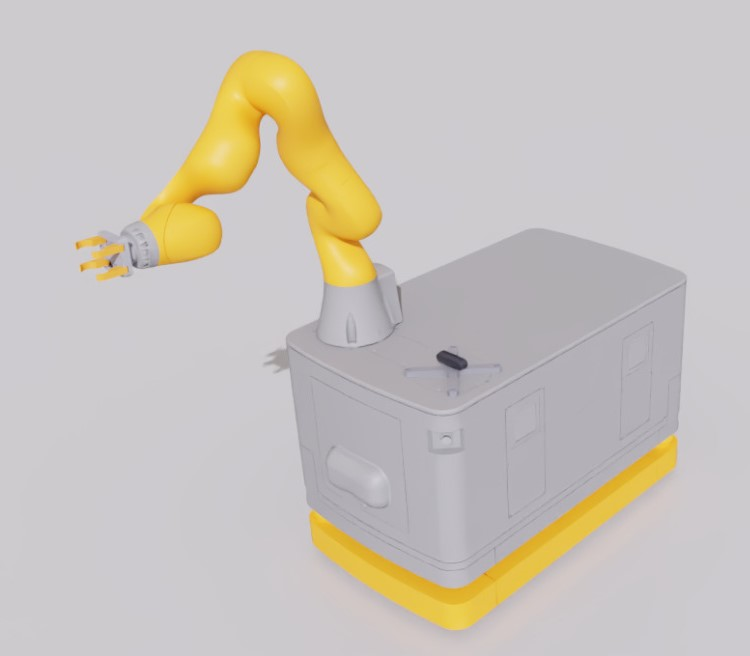
\includegraphics[width=0.7\textwidth]{figures/kmr_iiwa_isaac.jpg}
    \caption{Mobilni manipulator KMR iiwa u simulacijskom okruženju}
    \label{fig:kmr-iiwa}
\end{figure}

\subsection{Mobilna platforma}
\label{sec:platforma}

Platforma se giba pomoću četiriju Mecanum kotača (slika \ref{fig:mecanum-wheel}). Svaki se kotač sastoji od niza valjaka
postavljenih pod kutom od 45\textdegree{}{} u odnosu na os kotača, čime se postiže
omnidirekcijsko gibanje --- platforma se može gibati u proizvoljnom smjeru u ravnini i
istovremeno se zakretati, bez potrebe za promjenom orijentacije prije translacije. Ta je
osobina bitna za zadatak otvaranja vrata, jer omogućuje da baza slijedi luk krila bez
manevriranja. Tehnički podaci mobilne platforme nalaze se u tablici \ref{tab:platforma}.

\begin{figure}[H]
    \centering
    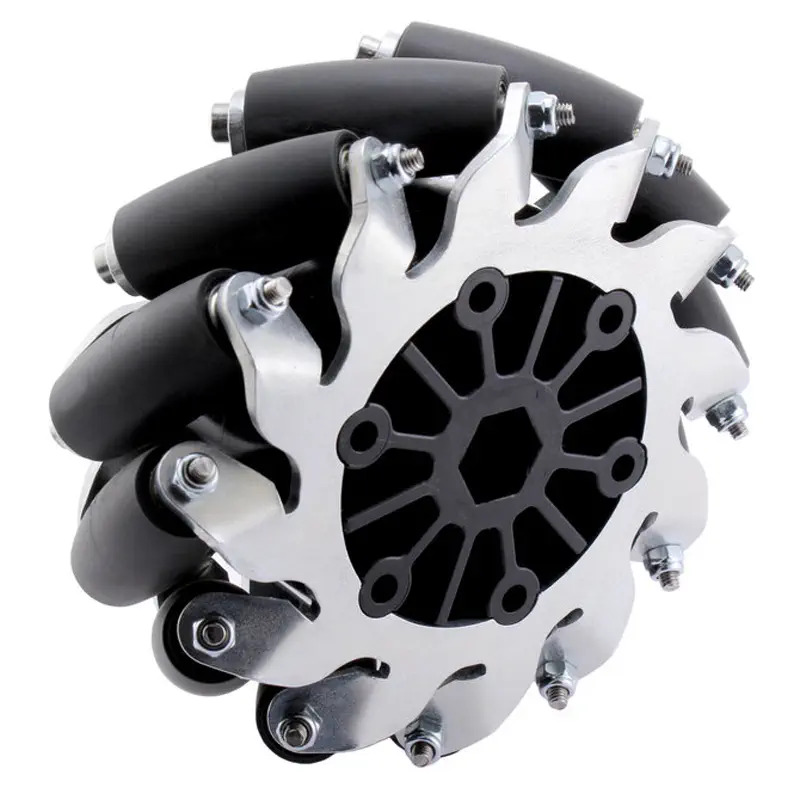
\includegraphics[width=0.45\textwidth]{figures/mecanum.jpg}
    \caption[Građa Mecanum kotača]{Građa Mecanum kotača \cite{mecanumsource}}
    \label{fig:mecanum-wheel}
\end{figure}

\begin{table}[H]
    \centering
    \caption{Tehnički podaci mobilne platforme}
    \label{tab:platforma}
    \begin{tabular}{@{}ll@{}}
        \toprule
        Veličina                                & Vrijednost                            \\
        \midrule
        Dimenzije (V\,$\times$\,Š\,$\times$\,D) & 700\,$\times$\,1080\,$\times$\,630 mm \\
        Masa                                    & 390 kg                                \\
        Najveća nosivost                        & 170 kg (200 kg bez manipulatora)      \\
        Brzina u uzdužnom smjeru                & najviše 3.6 km/h                      \\
        Brzina u poprečnom smjeru               & najviše 2.0 km/h                      \\
        Promjer kotača                          & 250 mm                                \\
        Klasa čistoće                           & ISO 5                                 \\
        \bottomrule
    \end{tabular}
\end{table}

\subsection{Manipulator LBR iiwa 7 R800}
\label{sec:lbr}

Korišten je manipulator LBR iiwa 7 R800, redundantna kinematička struktura sa sedam
rotacijskih osi. Za ovaj je rad ključno da manipulator ima senzor momenta u svakoj osi, što
omogućuje procjenu sile i momenta na vrhu alata bez zasebnog senzora sile na zapešću.
Postupak te procjene opisan je u poglavlju \ref{ch:procjena}. Sedma os čini strukturu
redundantnom u odnosu na šest stupnjeva slobode zadatka, pa isti položaj i orijentaciju vrha
alata ostvaruje kontinuum konfiguracija --- svojstvo koje se u poglavlju \ref{ch:rezultati}
pokazalo dosta važnim. Tehnički podaci manipulatora nalaze se u tablici \ref{tab:lbr}.

\begin{table}[H]
    \centering
    \caption{Tehnički podaci manipulatora LBR iiwa 7 R800}
    \label{tab:lbr}
    \begin{tabular}{@{}ll@{}}
        \toprule
        Veličina                    & Vrijednost         \\
        \midrule
        Nazivna nosivost            & 7 kg               \\
        Broj osi                    & 7                  \\
        Doseg                       & 800 mm             \\
        Izvedba zapešća             & u liniji           \\
        Prirubnica na osi 7         & DIN ISO 9409-1-A50 \\
        Ponovljivost pozicioniranja & $\pm$0.1 mm        \\
        Točnost momenta po osi      & $\pm$2 \%          \\
        Masa                        & 23.9 kg            \\
        Stupanj zaštite             & IP54               \\
        Položaj ugradnje            & pod, strop, zid    \\
        \bottomrule
    \end{tabular}
\end{table}

Granični momenti pojedinih zglobova navedeni su u tablici \ref{tab:momenti}.

\begin{table}[H]
    \centering
    \caption{Granični momenti zglobova manipulatora}
    \label{tab:momenti}
    \begin{tabular}{@{}lccccccc@{}}
        \toprule
        Zglob               & 1   & 2   & 3   & 4   & 5   & 6  & 7  \\
        \midrule
        Granični moment, Nm & 176 & 176 & 110 & 110 & 110 & 40 & 40 \\
        \bottomrule
    \end{tabular}
\end{table}

\section{Prihvatnica}
\label{sec:gripper}

Za hvatanje kvake izrađena je prilagođena prihvatnica (slika \ref{fig:gripper-render}). Budući da se rad provodi isključivo u
simulaciji, a stvarni prihvatni uređaj nije bio zadan, prihvatnica je oblikovana kao
zamjenjiva komponenta, tj. upravljanje njome potpuno je odvojeno od ostatka softvera
(potpoglavlje \ref{sec:ros2}), pa se može zamijeniti bez izmjena u ostatku sustava.

Prihvatnica ima četiri prsta raspoređena u dva para koja se zatvaraju duž osi $x$ baze, dok
uhvaćena šipka leži duž osi $y$. Svaki prst na sebi ima utor čiji je unutarnji luk prilagođen
šipki kvake promjera 28 mm. Pri potpuno zatvorenom hvatu otvor između prstiju uži je od šipke,
pa hvat ne počiva na geometrijskom dosjedanju nego na sili pogona i popustljivosti prstiju.
Time se izbjegava zazor koji bi pri vučenju vrata dopustio da se kvaka pomiče unutar hvata.
Položaj vrha alata (\textit{TCP}, engl. \textit{tool center point}) može se vidjeti na slici \ref{fig:gripper-tcp}.
Značajke prihvatnice nalaze se u tablici \ref{tab:gripper}.

Parovi prstiju ne gibaju se savršeno simetrično, pa se predmet ne centrira sam od sebe.
Ta se asimetrija ne pokušava ukloniti, nego se mjeri: tijekom prilaza kvaki uspoređuju se
položaji suprotnih prstiju i iz razlike se izračunava bočna korekcija kojom se prihvatnica
poravna nad kvakom prije nego što se hvat zatvori. Postupak je opisan u potpoglavlju
\ref{sec:prilaz}.

\begin{figure}[H]
    \centering
    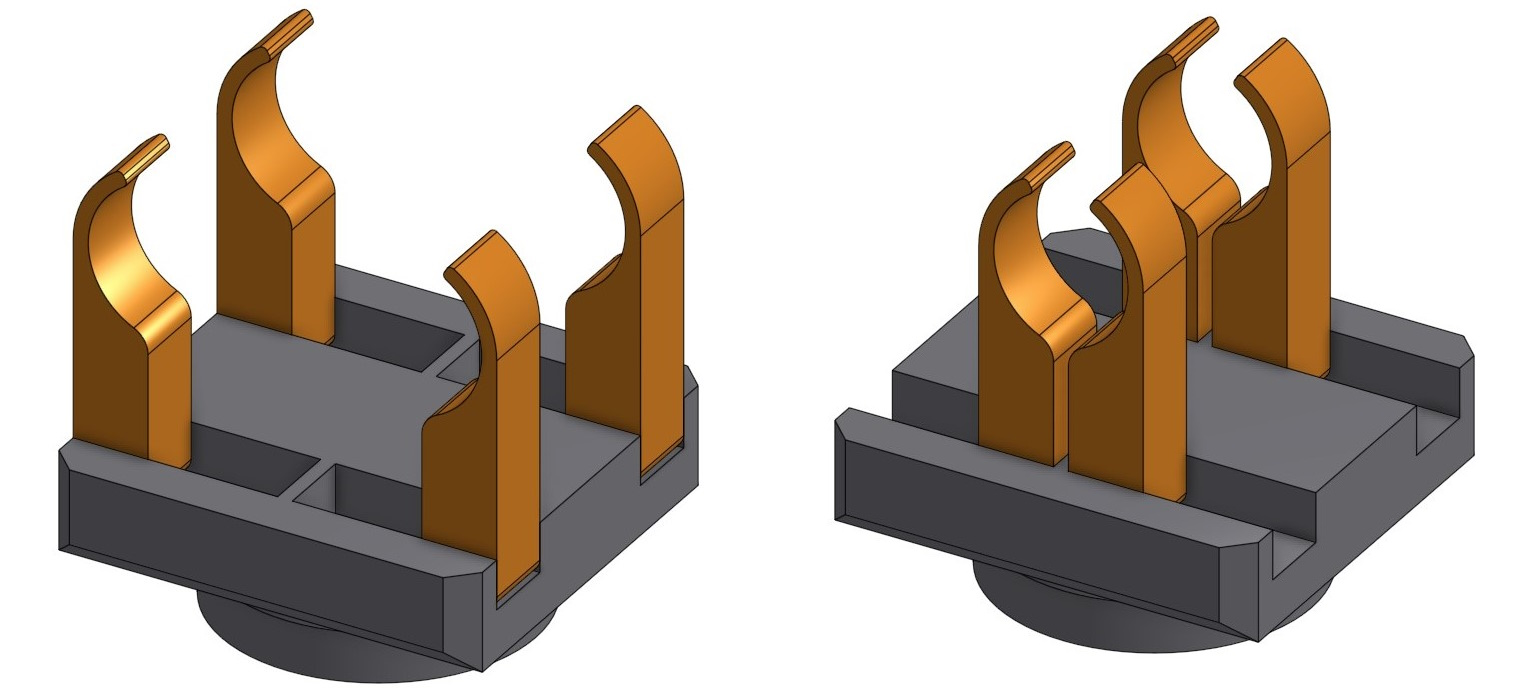
\includegraphics[width=0.75\textwidth]{figures/gripper_dual.jpg}
    \caption{Prihvatnica s četiri prsta; otvorena (lijevo) i zatvorena (desno)}
    \label{fig:gripper-render}
\end{figure}

\begin{figure}[H]
    \centering
    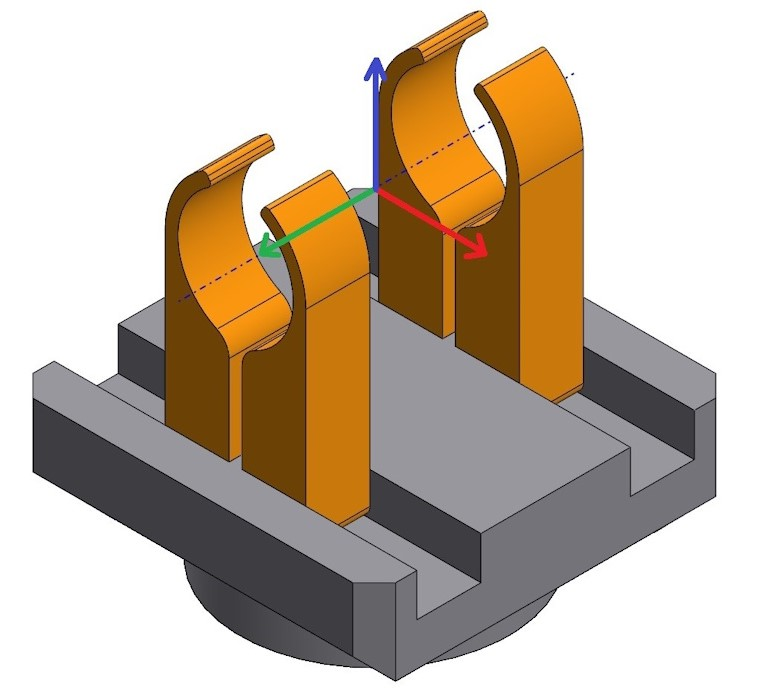
\includegraphics[width=0.45\textwidth]{figures/gripper_tcp.jpg}
    \caption{Položaj vrha alata (\textit{TCP})}
    \label{fig:gripper-tcp}
\end{figure}

\begin{table}[H]
    \centering
    \caption{Značajke prihvatnice}
    \label{tab:gripper}
    \begin{tabular}{@{}ll@{}}
        \toprule
        Značajka                             & Vrijednost          \\
        \midrule
        Promjer prirubnice                   & 63 mm               \\
        Dimenzije nosive ploče               & 85\,$\times$\,85 mm \\
        Duljina prsta                        & 66.5 mm             \\
        Unutarnji polumjer utora             & 16 mm               \\
        Hod po prstu                         & 0--25 mm            \\
        Masa nosivog dijela                  & 442 g               \\
        Masa prsta                           & 30.6 g              \\
        Ukupna masa                          & 564 g               \\
        Položaj vrha alata iznad prirubnice  & 74.85 mm            \\
        Statički koeficijent trenja prstiju  & 1.2                 \\
        Dinamički koeficijent trenja prstiju & 1.0                 \\
        \bottomrule
    \end{tabular}
\end{table}

Vrh alata leži na osi alata, na visini od 74.85 mm iznad prirubnice manipulatora. Ta visina
odgovara središtu unutarnjeg luka kuka pri zatvorenom hvatu, dakle visini na kojoj se nalazi
os uhvaćene šipke. Vrh alata time nije materijalna točka na prihvatnici, nego sjecište osi
alata i osi predmeta u hvatu, čime regulator momente računa oko stvarnog hvatišta.

Prsti su u simulacijskom modelu upravljani pozicijski, s krutošću pogona 20\,000 N/m,
prigušenjem 200 Ns/m i graničnom silom 600 N. Pri vučenju vrata silu prenose djelotvorno samo
dva od četiriju prstiju, jer jedan par radi protiv vlastitog pogona, pa je djelotvorna krutost
hvata polovica nominalne. Ta je pojedinost bitna za tumačenje rezultata u poglavlju
\ref{ch:rezultati}.

\section{Kamera i njezin nosač}
\label{sec:kamera-nosac}

Za detekciju kvake robot je opremljen kamerom Intel RealSense D435, postavljenom na mobilnu
platformu pomoću vlastito izrađenog nosača (slika \ref{fig:camera-mount}).
Sam postupak detekcije i procjene poze opisan je u poglavlju \ref{ch:percepcija};
ovdje je opisana samo montaža i pripadni koordinatni sustavi.

Nosač kamere oblikovan je tako da iskoristi postojeće provrte na platformi. Manipulator se na
platformu pričvršćuje preko četiri provrta promjera 13.3 mm raspoređena po kružnici polumjera
108 mm. Ta je kružnica na platformi izvedena zrcalno s obje strane, a strana suprotna
manipulatoru ostaje slobodna, pa je nosač kamere postavljen upravo na nju. Time montaža ne
zahtijeva nikakvu izmjenu platforme.

\begin{figure}[H]
    \centering
    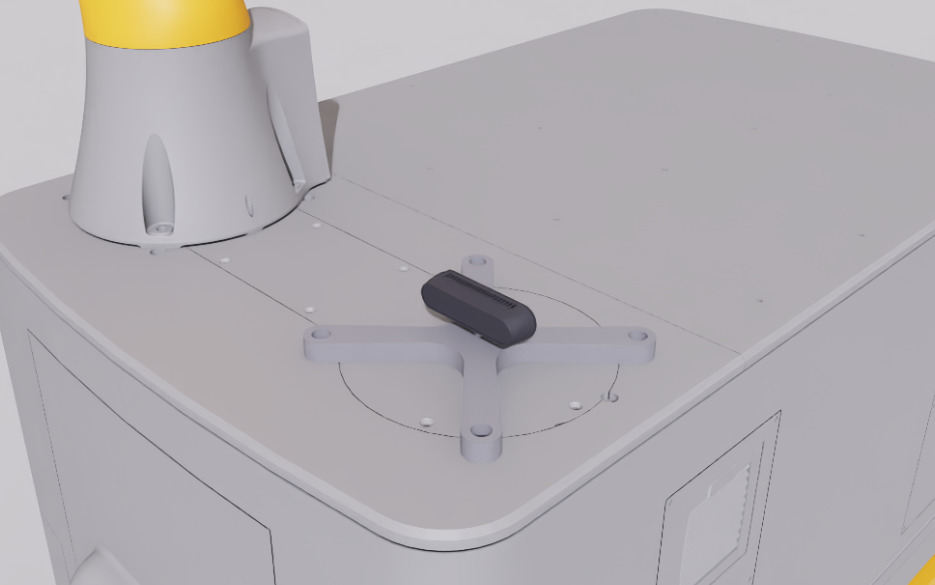
\includegraphics[width=0.7\textwidth]{figures/camera.jpg}
    \caption{Kamera i nosač kamere postavljeni na robotu}
    \label{fig:camera-mount}
\end{figure}

Kamera je smještena na visini gornje plohe platforme, bočno pomaknuta u odnosu na
manipulator. Time je kvaka u vidnom polju i tijekom prilaza i tijekom hvata, a kamera ne
ulazi u radni prostor manipulatora. Nosač je zamišljen kao izradak aditivnom proizvodnjom;
masa od 193 g izračunata je iz obujma modela uz gustoću materijala PETG od
1270 kg/m\textsuperscript{3}.

Kamera u modelu ima dva koordinatna sustava. Prvi je vezan uz kućište i služi za montažu,
a drugi je optički koordinatni sustav u kojem se izražavaju rezultati detekcije. Optički je
zaokrenut u odnosu na kućište prema uobičajenoj konvenciji, pri čemu os $z$ gleda u smjeru
promatranja, a osi $x$ i $y$ leže u ravnini slike. Ta konvencija nije proizvoljna nego je
očekuju biblioteke za obradu slike, pa je zadržana kako procjena poze ne bi zahtijevala
dodatnu pretvorbu.

Kamera podržava i dubinsku sliku, no ona u ovom radu nije korištena. Detekcija vrata i kvake
odvija se isključivo iz slike u boji, pomoću oznaka AprilTag, a postignuta točnost pokazala se
dovoljnom i bez dubinske informacije.

\section{Lidar}
\label{sec:lidar}

Uz kameru, robot je opremljen i dvodimenzijskim laserskim skenerom (lidarom), postavljenim na
prednjoj strani mobilne platforme. Za razliku od kamere, koja služi isključivo detekciji kvake
(poglavlje \ref{ch:percepcija}), lidar se koristi za dvije zadaće vezane uz neposrednu okolinu robota:
otkrivanje prepreka ispred platforme tijekom otvaranja vrata i pronalaženje otvora u zidu radi
prolaska kroz vrata. Obje su zadaće opisane u poglavlju \ref{ch:klasicni}, u opsegu klasičnog
pristupa; pristup temeljen na učenju ne koristi lidar direktno, već očitava pozicije zidova
izravno iz simulatora.

Senzor ima i minimalni domet ispod kojeg mjerenja nisu pouzdana. Budući da je kvaka nakon hvata
na udaljenosti od tek oko 0.65 m od senzora, unutar tog dometa krilo vrata ostaje nevidljivo, pa
je vrijednost minimalnog dometa u konfiguraciji senzora spuštena na 0.05 m.

\section{Modeli vrata}
\label{sec:vrata}

Radnu okolinu čine dva modela vrata, zakretna i klizna (slika \ref{fig:vrata}). Oba su izgrađena od osnovnih
geometrijskih tijela, s istim krilom, a razlikuju se stupnjem slobode gibanja i oblikom
kvake. Zajednička geometrija je namjerna: razlika u ponašanju dvaju pristupa time se ne može
pripisati razlici u dimenzijama ili masi krila.
Geometrijska i inercijska svojstva vrata mogu se vidjeti u tablici \ref{tab:vrata}.

\begin{figure}[H]
    \centering
    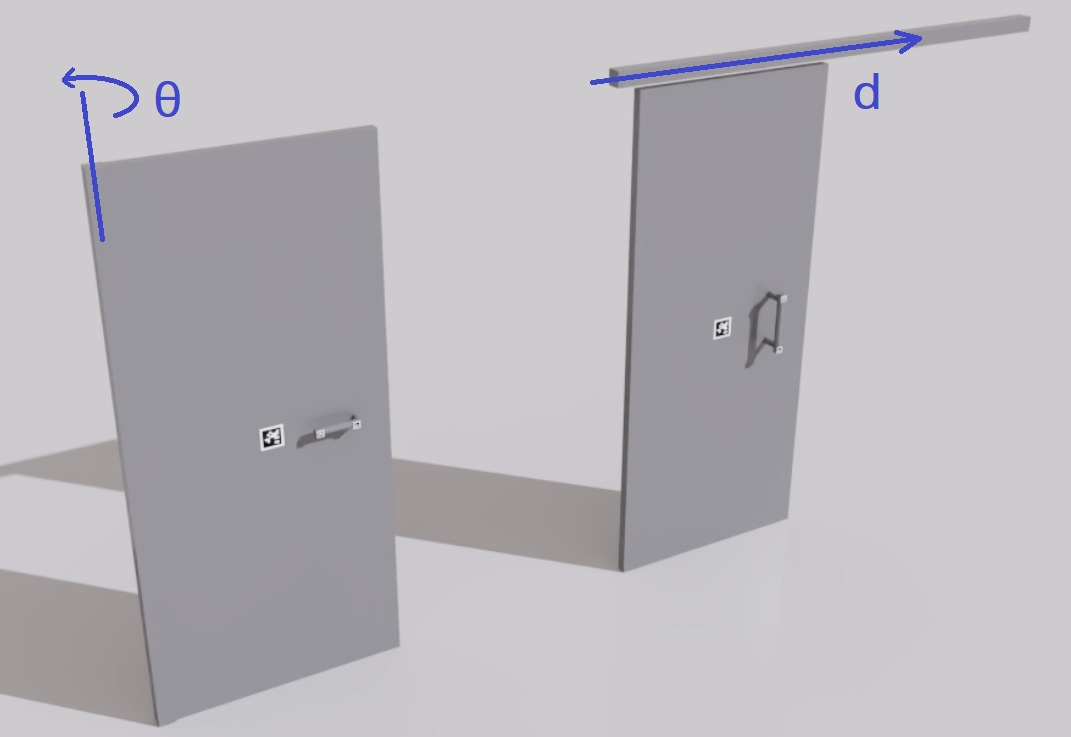
\includegraphics[width=0.9\textwidth]{figures/doors.jpg}
    \caption{Modeli zakretnih i kliznih vrata s označenim stupnjem slobode gibanja}
    \label{fig:vrata}
\end{figure}

\begin{table}[H]
    \centering
    \caption{Geometrija i inercijska svojstva modela vrata}
    \label{tab:vrata}
    \begin{tabular}{@{}lll@{}}
        \toprule
        Veličina             & Zakretna vrata                           & Klizna vrata                                 \\
        \midrule
        Krilo, dimenzije     & 40\,$\times$\,850\,$\times$\,2000 mm     & 40\,$\times$\,850\,$\times$\,2000 mm         \\
        Krilo, masa          & 15 kg                                    & 15 kg                                        \\
        Nepomični dio        & stup 60\,$\times$\,60\,$\times$\,2000 mm & vodilica 60\,$\times$\,2000\,$\times$\,60 mm \\
        Stupanj slobode      & rotacija oko osi $z$                     & translacija duž osi $y$                      \\
        Raspon gibanja       & 0--135 \textdegree{}                     & 0--1.0 m                                     \\
        Kvaka, oblik         & poluga, duljina 160 mm                   & šipka, duljina 250 mm                        \\
        Kvaka, promjer šipke & 28 mm                                    & 28 mm                                        \\
        Kvaka, masa          & 0.35 kg                                  & 0.35 kg                                      \\
        Visina hvatišta      & 1000 mm                                  & 1000 mm                                      \\
        \bottomrule
    \end{tabular}
\end{table}

Kod zakretnih vrata kvaka je izvedena kao poluga usmjerena prema osi šarke, kako je uobičajeno
kod stvarnih vrata. Zglob brave, koji bi omogućio zakretanje kvake, zavaren je u nepomični
zglob u oba pristupa, pa je jedini pokretni stupanj slobode zakretnih vrata os šarke.
Okretanje kvake time je izvan opsega rada; razlog i posljedice te odluke navedeni su u
potpoglavlju \ref{sec:klasicni-limits}. Posljedica koju treba imati na umu jest da se cijeli
moment šarke prenosi trenjem prstiju na šipki kvake.

Kod kliznih vrata kvaka je okomita šipka pričvršćena dvama odstojnicima, pa je hvatište
dostupno s prednje strane krila po cijeloj visini šipke.

Vrata su s obje strane omeđena zidom, izvedenim kao dva zasebna, nepomična elementa,
svaki dimenzija 0.06\,$\times$\,2.5\,$\times$\,2.0 m i mase 15 kg.
Zidovi su postavljeni tako da između njih ostaje slobodan prolaz od 0.85 m,
jednak širini krila vrata, čime nastaje realistična okolina vrata umjesto izoliranog objekta u
praznom prostoru. Ta je okolina preduvjet za dvije zadaće opisane u poglavlju
\ref{ch:klasicni}. Lidar treba stvarnu prepreku da bi u njoj prepoznao otvor, a MoveIt treba
stvarnu geometriju zida da bi je uzeo u obzir pri planiranju gibanja manipulatora.

\subsection{Otpor gibanja i njegova randomizacija}
\label{sec:otpor}

Otpor vrata nije zapisan u geometrijskom modelu, nego se postavlja pri svakom pokretanju
epizode iz zadanog raspona. Time politika nije vezana uz jednu vrijednost otpora, nego uči
raditi na rasponu vrata. Otpor je razdvojen na dva fizikalno različita člana:

\begin{equation}
    \tau_{\mathrm{otpor}} = \tau_{\mathrm{tr}} + d\,\dot{q} ,
    \label{eq:otpor}
\end{equation}

gdje je $q$ koordinata jedinog stupnja slobode vrata, dakle kut zakreta krila kod zakretnih
odnosno pomak krila kod kliznih vrata, a $\dot{q}$ njegova derivacija po vremenu, to jest
brzina otvaranja. Član $\tau_{\mathrm{tr}}$ Coulombovo je trenje, konstantno po iznosu i
neovisno o brzini, dok je $d$ koeficijent viskoznog prigušenja, koji daje otpor razmjeran
brzini. Izraz je zapisan općenito za oba tipa vrata: kod zakretnih su $\tau_{\mathrm{otpor}}$
i $\tau_{\mathrm{tr}}$ momenti, a kod kliznih sile.

Parametri se zadaju u apsolutnim jedinicama, dakle u njutnima za prizmatični i njutnmetrima za
revolutni zglob, a ne kao bezdimenzijski koeficijenti. Da bi se to potvrdilo, provedeno je
mjerenje u simulaciji. Vratima je zadana poznata vrijednost trenja, a zatim je polagano rastućom
silom određena sila pri kojoj se vrata pokrenu. Omjer izmjerene sile pokretanja i zadanog trenja
kretao se između 1.00 i 1.03 za zadane vrijednosti trenja u rasponu od 5 do 60 N, čime
je potvrđeno da zadana vrijednost izravno odgovara sili potrebnoj za pokretanje vrata.

U tablici \ref{tab:randomizacija} mogu se vidjeti rasponi iz kojih su birane vrijednosti otpora vrata:

\begin{table}[H]
    \centering
    \caption{Rasponi randomizacije otpora vrata}
    \label{tab:randomizacija}
    \begin{tabular}{@{}lcc@{}}
        \toprule
        Tip vrata & Trenje    & Prigušenje     \\
        \midrule
        Klizna    & 5--60 N   & 5--50 Ns/m     \\
        Zakretna  & 0.5--5 Nm & 0.5--5 Nms/rad \\
        \bottomrule
    \end{tabular}
\end{table}

Rasponi nisu određeni mjerenjem na stvarnim vratima, nego su usvojeni kao inženjerska
procjena, sa širinom raspona odabranom tako da obuhvati i lagana i teška vrata. Svrha im nije
vjerno preslikati određena vrata, već spriječiti da naučena politika ovisi o jednoj
vrijednosti otpora.

\section{Model robota i pretvorba u simulacijski format}
\label{sec:urdf-usd}

Geometrijski i kinematički model robota opisan je u formatu \textit{Unified Robot Description Format} (URDF). Model manipulatora preuzet
je iz javno dostupnog paketa \texttt{iiwa\_stack} \cite{iiwastack}, a model mobilne platforme
iz proizvođačeve dokumentacije \cite{kuka2024kmriiwa}. Prihvatnica, nosač kamere i oba modela
vrata izrađeni su u sklopu ovog rada. Model je organiziran pomoću \texttt{xacro} predložaka,
tako da se prihvatnica u model uključuje jednim pozivom makronaredbe.

Isaac Sim ne koristi URDF izravno, nego format \textit{Universal Scene Description} (USD). Pretvorba nije jedan korak nego niz
skripti, jer sama pretvorba ne prenosi sve što je za rad potrebno.

Osnovnu pretvorbu obavlja \texttt{convert\_urdf\_usd.py}, proširena inačica alata iz Isaac
Laba. Dvije su postavke pritom bitne:

\begin{itemize}
    \item \textbf{Vrsta kolidera} (engl. \textit{collider type})\textbf{.} Prsti prihvatnice
          moraju se pretvarati postupkom konveksne dekompozicije. Zamotavanje u konveksnu
          ovojnicu zatvorilo bi utore na prstima i prihvatnica ne bi mogla obuhvatiti šipku.
    \item \textbf{Sažimanje nepomičnih zglobova.} Ne smije se primijeniti na model robota, jer
          bi uklonilo zglob na kojem se očitavaju sile i momenti (potpoglavlje \ref{sec:gripper}).
\end{itemize}

Na dobiveni model zatim se primjenjuju tri naknadne skripte:

\begin{itemize}
    \item \texttt{apply\_gripper\_friction.py} pridružuje materijal trenja plohama prstiju i
          kvaka. Pridruživanje se ne može izvesti izravno na složenoj sceni, jer se geometrija
          prsta, referencirana četiri puta iz iste datoteke, pojavljuje kao instancirani sloj u
          koji nije dopušteno upisivati; skripta zato pronalazi stvarni sloj u kojemu se geometrija
          nalazi i materijal upisuje u njega.
    \item \texttt{add\_arm\_ros\_control\_graph.py} umeće graf koji povezuje zglobove
          manipulatora s temama ROS-a 2, čime se model može voditi izvana. Graf mora biti
          ugniježđen unutar stabla osnovnog elementa modela, jer se inače pri referenciranju
          modela u scenu tiho izgubi.
    \item \texttt{add\_camera\_ros\_graph.py} dodaje kameru s izmjerenim unutarnjim parametrima i
          položajem te objavljivanje slike i stabla koordinatnih sustava.
\end{itemize}

Na slici \ref{fig:urdf-usd-pipeline} može se vidjeti dijagram toka pretvorbe datoteka iz URDF formata u
simulatoru koristive datoteke u USD formatu.

\begin{figure}[H]
    \centering
    \begin{tikzpicture}[
            font        = \small,
            box/.style  = {draw, rounded corners=2pt, align=center, inner sep=4pt,
                    minimum height=9mm, minimum width=48mm, fill=black!5},
            data/.style = {box, fill=black!10},
            small/.style= {box, minimum width=44mm, minimum height=8mm},
            note/.style = {font=\scriptsize, align=left, anchor=west, text width=30mm},
            grp/.style  = {draw, dashed, rounded corners=3pt, inner sep=6pt},
            gl/.style   = {font=\scriptsize\itshape, anchor=east},
            ar/.style   = {-{Stealth[length=2mm]}, semithick}
        ]

        % ---------------- robot ----------------
        \node[data]  (rxacro) at (-3.0,0)     {predlošci \texttt{xacro}\\[-1pt]
            \scriptsize robot, prihvatnica, nosač kamere};
        \node[data]  (rurdf)  at (-3.0,-1.9)  {opis robota \texttt{URDF}};
        \node[box]   (rconv)  at (-3.0,-3.8)  {\texttt{convert\_urdf\_usd.py}};
        \node[data]  (rusd0)  at (-3.0,-5.7)  {osnovni model robota \texttt{USD}};

        \node[small] (fric) at (-3.0,-7.7)  {\texttt{apply\_gripper\_friction.py}};
        \node[small] (rosg) at (-3.0,-9.1)  {\texttt{add\_arm\_ros\_control\_graph.py}};
        \node[small] (camg) at (-3.0,-10.5) {\texttt{add\_camera\_ros\_graph.py}};
        \node[grp, fit=(fric)(rosg)(camg)] (gpost) {};
        \node[gl] at (gpost.west) {naknadna obrada};

        \node[data] (rusd1) at (-3.0,-12.6) {potpuni model robota \texttt{USD}};

        % ---------------- vrata ----------------
        \node[data, minimum width=44mm] (durdf) at (4.6,-5.7)
        {opis vrata \texttt{URDF}\\[-1pt]\scriptsize zakretna i klizna};
        \node[box,  minimum width=44mm] (dconv) at (4.6,-7.6)
        {\texttt{convert\_urdf\_usd.py}};
        \node[data, minimum width=44mm] (dusd)  at (4.6,-9.6)
        {modeli vrata \texttt{USD}\\[-1pt]\scriptsize inačice s oznakama i bez njih};

        % ---------------- izlazi ----------------
        \node[box, minimum width=42mm] (basej) at (-6.2,-14.8)
        {\texttt{add\_base\_joints.py}\\[-1pt]\scriptsize tri pomoćna zgloba platforme};
        \node[data, minimum width=42mm] (rlasset) at (-6.2,-16.9)
        {model za učenje\\[-1pt]\scriptsize \texttt{kmr\_iiwa\_full\_rl.usd}};

        \node[box, minimum width=52mm] (bis) at (0.9,-14.8)
        {\texttt{build\_integration\_scene.py}\\[-1pt]\scriptsize dodavanje podloge scene};
        \node[data, minimum width=52mm] (scene) at (0.9,-16.9)
        {integracijska scena\\[-1pt]\scriptsize \texttt{integration\_test\_*.usd}};

        % ---------------- tok ----------------
        \draw[ar] (rxacro) -- (rurdf);
        \draw[ar] (rurdf)  -- (rconv);
        \draw[ar] (rconv)  -- (rusd0);
        \draw[ar] (rusd0)  -- (gpost.north -| rusd0.south);
        \draw[ar] (fric)   -- (rosg);
        \draw[ar] (rosg)   -- (camg);
        \draw[ar] (gpost.south -| rusd1.north) -- (rusd1);

        \draw[ar] (durdf) -- (dconv);
        \draw[ar] (dconv) -- (dusd);

        \draw[ar] (rusd1.south) -- ++(0,-0.9) -| (basej.north);
        \draw[ar] (rusd1.south) -- ++(0,-0.9) -| (bis.north);
        \draw[ar] (basej) -- (rlasset);
        \draw[ar] (bis)   -- (scene);
        \draw[ar] (dusd.south) -- (4.6,-14.8) -- (bis.east);

        % ---------------- napomene ----------------
        \node[note] at (-0.4,-2.85) {sažimanje makronaredbi};
        \node[note] at (-0.4,-4.75) {konveksna dekompozicija kolidera;
            bez sažimanja nepomičnih zglobova};

    \end{tikzpicture}
    \caption{Postupak izrade simulacijskog modela iz opisa robota i vrata}
    \label{fig:urdf-usd-pipeline}
\end{figure}

Za učenje se koristi zasebna inačica modela. Iz modela vrata uklonjeni su nosivi elementi
oznaka za percepciju, jer tijela mase 0.001 kg uz krilo mase 15 kg loše uvjetuju numerički
postupak rješavanja. Nazivi članaka i zglobova ujednačeni su između obaju tipova vrata, čime
jedna programska implementacija okruženja poslužuje oba tipa bez grananja po tipu vrata.

\subsection{Gibanje mobilne platforme}
\label{sec:baza-model}

Mecanum kotači nisu simulirani kao tijela u kontaktu s podlogom. Umjesto toga, gibanje
platforme zadaje se kinematički: naredba brzine iz poruke \texttt{/cmd\_vel} pretvara se u
pomake platforme po osima $x$ i $y$ te zakret oko osi $z$. U okruženju za učenje isti je
mehanizam ostvaren trima pomoćnim zglobovima umetnutima između nepomičnog ishodišta i članka
platforme, pa se platforma giba kao dio iste kinematičke strukture kao i manipulator.

Korijen kinematičke strukture pritom ostaje nepomičan. To je nužno jer regulator u
operacijskom prostoru, opisan u poglavlju \ref{ch:rl}, računa jakobijan i matricu inercije uz
pretpostavku nepomičnog korijena; uz slobodan korijen kompenzacija gravitacije ispada
neispravna.

Zanemarivanje dinamike kotača pojednostavljenje je koje uklanja proklizavanje, elastičnost
valjaka i ograničenja pogona kotača. Za zadatak u kojem se platforma giba malim brzinama i u
kojem su zanimljive sile na vrhu alata, a ne na kotačima, to je prihvatljivo, ali ograničava
prenosivost rezultata na stvarnog robota. Ograničenje je navedeno u poglavlju
\ref{ch:zakljucak}.

\section{Simulacijsko okruženje}
\label{sec:isaac}

Simulacija se izvodi u okruženju NVIDIA Isaac Sim, uz biblioteku Isaac Lab
\cite{isaaclab} za paralelno učenje. Fizika se rješava pogonom PhysX. Cijeli je rad proveden u
simulaciji jer stvarni robot nije bio dostupan, a zadatak zahtijeva velik broj ponavljanja
interakcije s kontaktom, što na stvarnom robotu nije izvedivo u opsegu završnog rada.

Bitna je značajka postava razdvajanje odgovornosti: geometrijski model nosi topologiju i
geometriju, a sva pojačanja pogona i svojstva otpora zadaju se u konfiguraciji okruženja. Time
se izbjegava da se naučena politika veže uz jednu konkretnu datoteku modela umjesto uz raspon
uvjeta.

Pogoni osi manipulatora postavljeni su na nultu krutost i prigušenje. Momente računa regulator
u operacijskom prostoru i zadaje ih izravno; da je zadržana krutost iz pretvorbe, pogon i
regulator djelovali bi jedan protiv drugoga i krutost koju politika zada ne bi imala učinka.
Pogon platforme brzinski je, s prigušenjem $10^4$, a pogon prstiju pozicijski, s vrijednostima
navedenima u potpoglavlju \ref{sec:gripper}.

Programska i sklopovska konfiguracija može se vidjeti u tablici \ref{tab:okruzenje}.

\begin{table}[H]
    \centering
    \caption{Programska i sklopovska konfiguracija}
    \label{tab:okruzenje}
    \begin{tabular}{@{}ll@{}}
        \toprule
        Stavka                      & Vrijednost                         \\
        \midrule
        Operacijski sustav          & Ubuntu 22.04 LTS                   \\
        Simulator                   & NVIDIA Isaac Sim 5.1.0             \\
        Biblioteka za učenje        & Isaac Lab 2.3.2                    \\
        Robotski operacijski sustav & ROS 2 Humble                       \\
        Python (Isaac Lab)          & 3.11.15                            \\
        Python (ROS 2)              & 3.10.12                            \\
        \midrule
        Procesor                    & AMD Ryzen 7 260                    \\
        Grafička kartica            & NVIDIA GeForce RTX 5050, 8 GB VRAM \\
        Radna memorija              & 32 GB DDR5                         \\
        \bottomrule
    \end{tabular}
\end{table}

\section{Programska arhitektura}
\label{sec:ros2}

Softver je podijeljen u pakete unutar radnog prostora ROS 2, navedene u tablici
\ref{tab:paketi}. Podjela slijedi funkcionalne cjeline rada: opis robota, percepcija, veza sa
simulatorom, izvođenje zadatka, konfiguracija i pokretanje sustava.

\begin{table}[H]
    \centering
    \caption{Paketi radnog prostora ROS 2}
    \label{tab:paketi}
    \begin{tabular}{@{}ll@{}}
        \toprule
        Paket                              & Sadržaj                                                \\
        \midrule
        \texttt{kmr\_iiwa\_description}    & modeli robota, prihvatnice, kamere i vrata             \\
        \texttt{kmr\_iiwa\_perception}     & detekcija oznaka, fuzija poze, procjena sile i momenta \\
        \texttt{kmr\_iiwa\_sim\_bridge}    & veza sa simulatorom: platforma, prihvatnica, kamera    \\
        \texttt{kmr\_iiwa\_task}           & izvođenje zadatka i procjena ograničenja gibanja       \\
        \texttt{kmr\_iiwa\_moveit\_config} & konfiguracija planiranja gibanja manipulatora          \\
        \texttt{kmr\_iiwa\_bringup}        & pokretanje cjelokupnog sustava                         \\
        \bottomrule
    \end{tabular}
\end{table}

Isaac Sim nema izvornu podršku za sučelje \texttt{ros2\_control}, pa je veza sa simulatorom
ostvarena vlastito izrađenim čvorovima koji prevode poruke ROS 2 u naredbe simulatoru. Upravljanje
prihvatnicom namjerno je izvedeno kao potpuno odvojena cjelina: jedini čvor koji zna da
prihvatnica ima četiri prizmatična zgloba i hod od 25 mm jest njezin upravljački čvor, dok
ostatak sustava prihvatnicu vidi kroz jedan broj u rasponu od nula do jedan, uz povratnu
informaciju o trenutnom položaju i o tome je li zaustavljena prije dolaska u zadani položaj.
Time je zadovoljen zahtjev iz potpoglavlja \ref{sec:gripper} da se prihvatnica može zamijeniti
bez izmjena u ostatku sustava.

Na slici \ref{fig:arch-klasicni} može se vidjeti dijagram arhitekture za klasično učenje.

\begin{figure}[H]
    \centering
    \begin{tikzpicture}[
            font       = \small,
            box/.style = {draw, rounded corners=2pt, align=center, inner sep=4pt,
                    minimum height=9mm, fill=black!5},
            grp/.style = {draw, dashed, rounded corners=3pt, inner sep=7pt},
            gl/.style  = {font=\scriptsize\itshape, anchor=east},
            tl/.style  = {font=\scriptsize\ttfamily, fill=white, inner sep=1.5pt},
            ar/.style  = {-{Stealth[length=2mm]}, semithick}
        ]

        % --- simulator ---
        \node[box, minimum width=112mm, fill=black!10] (sim) at (0,0)
        {Isaac Sim --- scena: robot, vrata, fizika kontakta};

        % --- percepcija ---
        \node[box, minimum width=44mm] (tag) at (-2.6,-2.7)
        {detekcija oznaka\\i fuzija poze};
        \node[box, minimum width=40mm] (wr)  at ( 2.8,-2.7)
        {procjena sile\\i momenta};
        \node[grp, fit=(tag)(wr)] (gperc) {};
        \node[gl] at (gperc.west) {\texttt{kmr\_iiwa\_perception}};

        % --- zadatak ---
        \node[box, minimum width=50mm] (task) at (-2.2,-5.8)
        {izvođenje zadatka\\[-1pt]\scriptsize prilaz, hvat, procjena, otvaranje};
        \node[box, minimum width=30mm] (moveit) at (3.6,-5.8) {MoveIt 2\\planiranje};
        \node[grp, fit=(task)] (gtask) {};
        \node[gl] at (gtask.west) {\texttt{kmr\_iiwa\_task}};

        % --- most prema simulatoru ---
        \node[box, minimum width=26mm] (cmdvel) at (-3.6,-8.8) {platforma};
        \node[box, minimum width=26mm] (grip)   at ( 0.0,-8.8) {prihvatnica};
        \node[box, minimum width=26mm] (armg)   at ( 3.6,-8.8) {manipulator};
        \node[grp, fit=(cmdvel)(grip)(armg)] (gbridge) {};
        \node[gl] at (gbridge.west) {\texttt{kmr\_iiwa\_sim\_bridge}};

        % --- simulator -> percepcija ---
        \draw[ar] (sim.south -| tag.north) -- (tag.north);
        \draw[ar] (sim.south -| wr.north)  -- (wr.north);
        \node[tl] at (-2.6,-1.35) {/camera/color/image\_raw};
        \node[tl] at ( 2.8,-1.35) {/joint\_states};

        % --- simulator -> zadatak (lidar, izravno, bez zasebnog obradnog čvora) ---
        \draw[ar] (sim.south -| 5.2,0) -- (5.2,-4.6) -- (1.2,-4.6) -- (1.2,-5.8) -- (task.east);
        \node[tl] at (3.2,-4.6) {/scan};

        % --- percepcija -> zadatak ---
        \draw[ar] (tag.south) -- (tag.south |- gtask.north);
        \draw[ar] (wr.south) -- ++(0,-1.1) -| ($(task.north)+(1.6,0)$);
        \node[tl] at (-2.6,-4.25) {/perception/handle\_pose};
        \node[tl] at ( 2.8,-4.25) {/estimation/tcp\_wrench};

        % --- zadatak <-> MoveIt ---
        \draw[{Stealth[length=2mm]}-{Stealth[length=2mm]}, semithick]
        (moveit.west) -- (task.east);

        % --- zadatak -> most ---
        \draw[ar] ($(task.south)+(-1.4,0)$) -- ++(0,-1.1) -| (cmdvel.north);
        \draw[ar] ($(task.south)+(1.4,0)$)  -- ++(0,-1.7) -| (grip.north);
        \draw[ar] (moveit.south) -- (armg.north);
        \node[tl] at (-3.6,-7.35) {/cmd\_vel};
        \node[tl] at ( 0.0,-7.35) {/gripper\_cmd};
        \node[tl] at ( 3.6,-7.35) {trajektorija};

        % --- most -> simulator (zatvaranje petlje desno) ---
        \draw[ar] (gbridge.east) -- ++(1.3,0) |- (sim.east);
        \node[tl, rotate=90] at (6.3,-4.4) {naredbe simulatoru};

    \end{tikzpicture}
    \caption{Programska arhitektura klasičnog pristupa}
    \label{fig:arch-klasicni}
\end{figure}

Pristup temeljen na učenju koristi bitno jednostavniju arhitekturu (slika \ref{fig:arch-rl}). Tijekom učenja ROS 2 nije
u regulacijskoj petlji: okruženje, regulator i politika izvode se unutar Isaac Laba, izravno
nad tenzorima na grafičkoj kartici. Razlog je paralelizacija --- učenje se izvodi u više
stotina istovremenih okruženja, a posredovanje kroz ROS 2 bilo bi usko grlo. Veza s ROS-om
potrebna je tek pri izvođenju naučene politike izvan simulacije, što nije bilo u opsegu ovog
rada i opisano je u poglavlju \ref{ch:rezultati}.

\begin{figure}[H]
    \centering
    \begin{tikzpicture}[
            font       = \small,
            box/.style = {draw, rounded corners=2pt, align=center, inner sep=4pt,
                    minimum height=9mm, minimum width=32mm, fill=black!5},
            grp/.style = {draw, dashed, rounded corners=3pt, inner sep=7pt},
            gl/.style  = {font=\scriptsize\itshape, anchor=east},
            tl/.style  = {font=\scriptsize, fill=white, inner sep=1.5pt},
            ar/.style  = {-{Stealth[length=2mm]}, semithick}
        ]

        \node[box, minimum width=104mm, fill=black!10] (phys) at (0,0)
        {PhysX --- $N$ paralelnih okruženja na grafičkoj kartici};

        \node[box] (obs) at (-3.4,-2.7) {opažanje};
        \node[box] (pol) at ( 0.0,-2.7) {politika\\[-1pt]\scriptsize neuronska mreža};
        \node[box] (act) at ( 3.4,-2.7) {akcija};
        \node[grp, fit=(obs)(pol)(act)] (gpol) {};
        \node[gl] at (gpol.west) {upravljačka petlja};

        \node[box, minimum width=54mm] (osc) at (1.0,-5.4)
        {regulator u operacijskom prostoru\\[-1pt]\scriptsize varijabilna impedancija};

        \node[box] (ppo) at (-2.6,-7.9) {PPO\\[-1pt]\scriptsize \texttt{rsl\_rl}};
        \node[box] (rew) at ( 3.0,-7.9) {nagrada};
        \node[grp, fit=(ppo)(rew)] (glearn) {};
        \node[gl] at (glearn.west) {učenje};

        % --- upravljačka petlja ---
        \draw[ar] (phys.south -| obs.north) -- (obs.north) node[tl, midway] {stanje};
        \draw[ar] (obs.east) -- (pol.west);
        \draw[ar] (pol.east) -- (act.west);
        \draw[ar] (act.south) -- (act.south |- osc.north)
        node[tl, midway] {pomak i krutost};

        % momenti: desnom stranom natrag u fiziku
        \draw[ar] (osc.east) -- (6.0,-5.4) -- (6.0,-0.225) -- (phys.east);
        \node[tl, rotate=90] at (6.0,-3.0) {momenti};

        % --- petlja učenja ---
        \draw[ar] (phys.east) ++(0,0.15) -- (7.4,0.15) -- (7.4,-7.9) -- (rew.east);
        \node[tl, rotate=90] at (7.4,-4.4) {napredak, sila};
        \draw[ar] (rew.west) -- (ppo.east);

        % ažuriranje: lijevom stranom, iznad regulatora
        \draw[ar] (ppo.north) -- (-2.6,-4.35) -- (0,-4.35) -- (pol.south);
        \node[tl] at (-1.3,-4.35) {ažuriranje težina};

    \end{tikzpicture}
    \caption{Programska arhitektura pristupa temeljenog na učenju}
    \label{fig:arch-rl}
\end{figure}
\chapter{MODUL PERCEPCIJE}
\label{ch:percepcija}

Zadatak modula percepcije jest odrediti položaj i orijentaciju hvatišta kvake iz slike, u
koordinatnom sustavu vezanom uz robota, kako bi se manipulator mogao voditi prema hvatištu bez
unaprijed poznatog položaja vrata. Fizička izvedba kamere i njezina montaža opisane su u
potpoglavlju \ref{sec:kamera-nosac}; ovdje je opisan postupak obrade slike i izlaz koji modul
daje ostatku sustava.

\section{Odabir pristupa}
\label{sec:pristup-percepcija}

Procjena poze provodi se pomoću vizualnih oznaka postavljenih na vrata i kvaku. Oznake su
odabrane jer daju potpunu procjenu poze s poznatom mjernom nesigurnošću iz jedne slike, bez
prethodnog učenja i bez skupa označenih primjera. To je u ovom radu bitno, jer je fokus
zadatka na upravljanju u kontaktu, a ne na prepoznavanju objekata; oznake omogućuju da modul
percepcije bude pouzdan ulaz za ostatak sustava, umjesto da sam postane predmet istraživanja.

Uporaba oznaka istovremeno je i najveće pojednostavljenje u radu. Stvarna vrata nemaju oznake,
pa robot s ovakvim modulom ne bi radio izvan pripremljene okoline. Postupci koji ne zahtijevaju
oznake postoje --- Stuede i suradnici za isti zadatak i isti tip robota kvaku detektiraju
konvolucijskom neuronskom mrežom \cite{stuede2019door} --- ali traže skup podataka i vrijeme
učenja koji nisu bili u opsegu ovog rada. Posljedice su navedene u potpoglavlju
\ref{sec:perception-limits}.

Od dviju uobičajenih obitelji oznaka odabran je AprilTag \cite{olson2011apriltag}, i to zbog
zrelijih detekcijskih biblioteka u sustavu ROS 2 te točnije procjene orijentacije pri malim
oznakama nego što je daju usporedive alternative.

\section{Raspored oznaka}
\label{sec:raspored-oznaka}

Na svakim vratima nalaze se tri oznake (slika \ref{fig:apriltags}), raspoređene prema tablici \ref{tab:oznake}. Podjela na
jednu veliku i dvije male oznake slijedi iz toga što prilaz i hvat imaju različite zahtjeve.

Velika oznaka na sredini krila služi fazi prilaza. Njezina veličina omogućuje pouzdanu
detekciju s udaljenosti od dva do tri metra, dakle iz položaja u kojem robot započinje
zadatak. U toj fazi nije potrebna velika točnost, nego samo dovoljno dobra procjena smjera i
udaljenosti da se platforma dovede pred vrata.

\begin{figure}[H]
    \centering
    
\includegraphics[width=0.4\textwidth]{figures/apriltags.jpg}
    \caption{AprilTagovi: sredina vrata (gore), kvaka (A dolje lijevo, B dolje desno)}
    \label{fig:apriltags}
\end{figure}

Dvije male oznake na krajevima kvake služe fazi hvata, na radnoj udaljenosti od otprilike
jednog do jednog i pol metra. Njihova je veličina ograničena promjerom šipke kvake, koji iznosi
28 mm, pa je za njih odabrana obitelj s mrežom $4 \times 4$ umjesto $6 \times 6$: pri istoj
duljini stranice takva oznaka ima krupnija polja i ostaje čitljiva na većoj udaljenosti.
Cijena je manja Hammingova udaljenost među kodovima, dakle veća sklonost lažnim detekcijama,
što je ublaženo time da modul očekuje unaprijed poznate identifikatore i provjerava je li
izmjereni razmak dviju oznaka u očekivanom rasponu.

\begin{table}[H]
    \centering
    \caption{Raspored vizualnih oznaka na vratima}
    \label{tab:oznake}
    \begin{tabular}{@{}lllll@{}}
        \toprule
        Oznaka     & Vrata    & Nosivi članak & Veličina & Obitelj  \\
        \midrule
        središnja  & oba      & krilo         & 80 mm    & tag36h11 \\
        kvaka, $A$ & zakretna & poluga kvake  & 25 mm    & tag16h5  \\
        kvaka, $B$ & zakretna & poluga kvake  & 25 mm    & tag16h5  \\
        kvaka, $A$ & klizna   & šipka kvake   & 25 mm    & tag16h5  \\
        kvaka, $B$ & klizna   & šipka kvake   & 25 mm    & tag16h5  \\
        \bottomrule
    \end{tabular}
\end{table}

Razmak dviju malih oznaka razlikuje se po tipu vrata i iznosi 130 mm na zakretnim te 220 mm na
kliznim vratima, jer je kod zakretnih vrata poluga kvake vodoravna i kraća, a kod kliznih je
šipka okomita i dulja. Raspored je prikazan na slici \ref{fig:oznake}.

\begin{figure}[H]
    \centering
    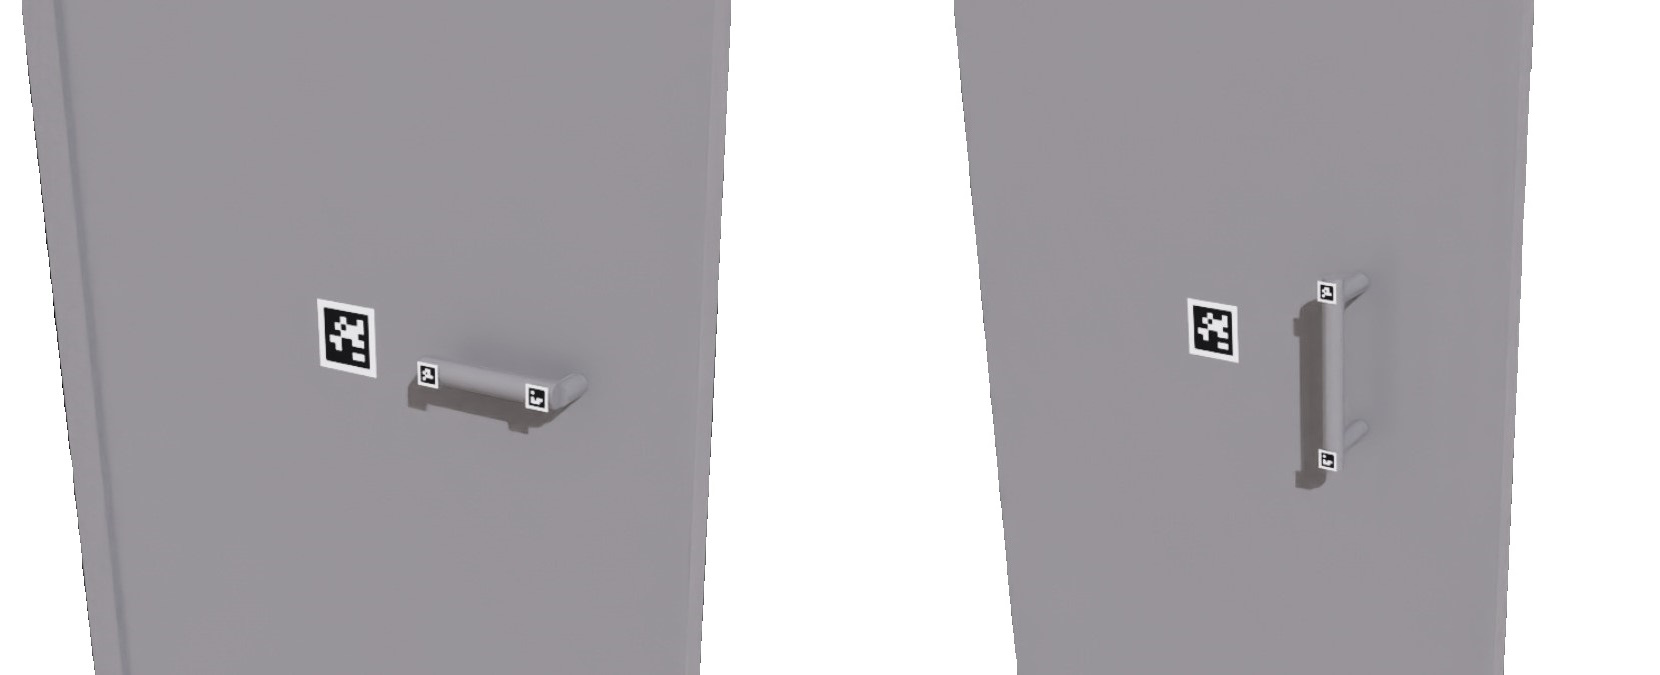
\includegraphics[width=0.9\textwidth]{figures/door_tags_dual.jpg}
    \caption{Raspored vizualnih oznaka na zakretnim (lijevo) i kliznim (desno) vratima}
    \label{fig:oznake}
\end{figure}

\section{Detekcija oznaka}
\label{sec:detekcija}

Detekcija se provodi gotovim paketom \texttt{apriltag\_ros} za sustav ROS 2, koji iz slike u boji i unutarnjih
parametara kamere daje potpunu pozu svake prepoznate oznake u optičkom koordinatnom sustavu
kamere. Kako jedan primjerak čvora obrađuje samo jednu obitelj oznaka, pokreću se dva
primjerka, po jedan za veliku i za male oznake.

Slika i unutarnji parametri kamere dolaze izravno iz simulatora, kao i cijelo stablo
koordinatnih sustava robota. Objavljivanje stabla nije samorazumljivo: uvoz modela ne stvara
ga sam od sebe, nego ga je trebalo dodati zasebno pri izradi simulacijskog modela
(potpoglavlje \ref{sec:urdf-usd}).

\section{Fuzija dviju oznaka na kvaki}
\label{sec:fuzija}

Poza kvake ne uzima se od pojedine oznake, nego se računa iz obiju. Razlog je osjetljivost
procjene orijentacije na veličinu oznake: pri stranici od 25 mm i udaljenosti od preko jednog
metra procjena orijentacije pojedine oznake znatno je nesigurnija od procjene položaja. Dvije
oznake razmaknute 130 odnosno 220 mm daju mjernu bazu red veličine dulju od stranice same
oznake, pa se smjer duž kvake iz njihovih položaja procjenjuje bitno pouzdanije nego iz
orijentacije bilo koje pojedine oznake.

Neka su $\bm{p}_A$ i $\bm{p}_B$ položaji dviju oznaka, a $\bm{z}_A$ i $\bm{z}_B$ njihove
normale, sve izraženo u koordinatnom sustavu robota. Položaj hvatišta uzima se kao polovište

\begin{equation}
    \bm{p} = \tfrac{1}{2} \left( \bm{p}_A + \bm{p}_B \right) .
    \label{eq:poloviste}
\end{equation}

Os $y$ hvatišta postavlja se duž kvake, iz razlike položaja dviju oznaka:

\begin{equation}
    \bm{e}_y = \frac{\bm{p}_B - \bm{p}_A}{\norm{\bm{p}_B - \bm{p}_A}} .
    \label{eq:osy}
\end{equation}

Preostale dvije osi izvode se iz normala oznaka. Njihova srednja vrijednost
$\bar{\bm{z}} = \tfrac{1}{2}(\bm{z}_A + \bm{z}_B)$ općenito nije okomita na $\bm{e}_y$, pa se
ortogonalizira Gram-Schmidtovim postupkom:

\begin{equation}
    \bm{e}_z = \frac{\bar{\bm{z}} - (\bar{\bm{z}} \cdot \bm{e}_y)\,\bm{e}_y}
    {\norm{\bar{\bm{z}} - (\bar{\bm{z}} \cdot \bm{e}_y)\,\bm{e}_y}} ,
    \qquad
    \bm{e}_x = \bm{e}_y \times \bm{e}_z .
    \label{eq:ortogonalizacija}
\end{equation}

Matrica rotacije hvatišta jest $\bm{R} = [\,\bm{e}_x \ \ \bm{e}_y \ \ \bm{e}_z\,]$. Ovakav
postupak nije usrednjavanje dviju poza, nego prilagodba krutog tijela dvjema izmjerenim
točkama, pri čemu se od pojedinih oznaka preuzima samo ono što one dobro mjere: položaj u
cijelosti, a od orijentacije samo normala.

Prije računanja provode se dvije provjere. Uspoređuju se vremenske oznake dviju detekcija, da
se ne spoje mjerenja iz različitih trenutaka, i provjerava se je li njihov razmak unutar
raspona od 50 do 400 mm, čime se odbacuju lažne detekcije. Usporedba vremenskih oznaka provodi
se međusobno, između dviju detekcija, a ne u odnosu na sat računala, jer simulator ne
objavljuje vlastito vrijeme, pa bi takva usporedba spajala dvije nepovezane vremenske domene.

\section{Sučelje modula i radni doseg}
\label{sec:perception-iface}

Modul objavljuje pozu hvatišta na jednoj temi, s frekvencijom od 10 Hz, izraženu u
koordinatnom sustavu platforme. Time je sučelje prema ostatku sustava svedeno na jednu poruku,
neovisno o tome koliko je oznaka i kojih obitelji upotrijebljeno, pa se postupak detekcije može
zamijeniti bez izmjena u kodu koji izvodi zadatak.

Dvije skupine oznaka imaju bitno različit radni doseg. Središnja oznaka pouzdano se detektira s
udaljenosti od dva do tri metra, pa pokriva cijelu fazu prilaza. Male oznake na kvaki traže
udaljenost manju od otprilike 1.2 m, i to ne zbog razlučivosti nego zbog vidnog polja: bliže
od te udaljenosti gornja oznaka izlazi iz kadra, a procjena smjera duž kvake gubi jednu od dviju
mjernih točaka i orijentacija hvatišta se raspada.

Ta udaljenost istovremeno je veća od dosega manipulatora pri nepomičnoj platformi, pa se poza
kvake očita s ruba radnog dosega, a platforma se tek nakon toga primakne. Kako platforma nema
odometriju, poza kvake pritom se rekonstruira iz njezina nepromjenjivog odnosa prema središnjoj
oznaci. Postupak je opisan u potpoglavlju \ref{sec:prilaz}.

\section{Preciznost percepcijskog modula}
\label{sec:perception-error}

Provedeno je testiranje točnosti i preciznosti percepcijskog modula, čiji se rezultati mogu
vidjeti u tablici \ref{tab:tocnost-percepcije} te na slici \ref{fig:perception-error}.
Testiranje je provedeno tako da se robot dovodio na nasumične pozicije ispred vrata tako da kamera
vidi oznake na kvaki. Zatim se uz pomoć vlastito izrađene skripte \texttt{perception\_accuracy\_logger.py}
očitala poza hvatišta koju daje percepcijski modul i uspoređivala sa stvarnom pozom dobivenom iz simulatora.
Postupak je ponovljen 15 puta za obje vrste vrata.

\begin{table}[H]
    \centering
    \caption{Točnost procjene poze hvatišta, 30 mjernih točaka}
    \label{tab:tocnost-percepcije}
    \begin{tabular}{@{}llccc@{}}
        \toprule
        Veličina                & Jedinica & Srednja vrijednost & Std. devijacija & Najveća \\
        \midrule
        Pogreška položaja       & mm       & 17.07              & 9.01            & 44.82   \\
        \quad okomito na kvaku  & mm       & 15.59              & 9.47            & 44.81   \\
        \quad duž kvake         & mm       & 5.74               & 2.70            & 11.95   \\
        Pogreška smjera kvake   & $^\circ$ & 2.13               & 2.82            & 11.48   \\
        Pogreška orijentacije   & $^\circ$ & 4.88               & 5.76            & 23.97   \\
        Rasip procjene položaja & mm       & 1.29               & 0.75            & 3.90    \\
        \bottomrule
    \end{tabular}
\end{table}

\begin{figure}[H]
    \centering
    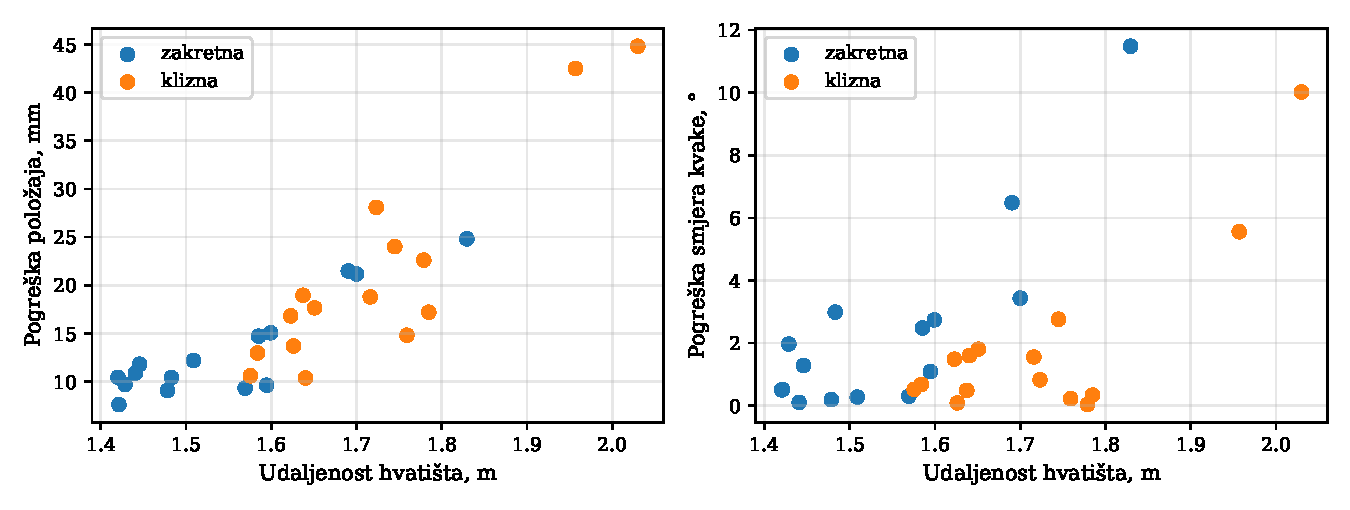
\includegraphics[width=\textwidth]{figures/perception_error_vs_distance.pdf}
    \caption{Ovisnost pogreške položaja i smjera kvake o udaljenosti hvatišta od robota}
    \label{fig:perception-error}
\end{figure}

Može se primijetiti da je odstupanje položaja i smjera kvake veće pri većim udaljenostima,
a pri manjim udaljenostima je pogreška svega desetak milimetara, odnosno par stupnjeva.
Kako se poza hvatišta traži tek kad je robot dovoljno blizu vratima (oko 1.2 m), pogreška
percepcije je dovoljno mala da ne igra veliku ulogu. Pogreška se kasnije kompenzira
prilikom faze hvata, kako je opisano u \ref{sec:gripper} i \ref{sec:prilaz}.

\section{Ograničenja}
\label{sec:perception-limits}

\textbf{Oznake na vratima.} Modul pretpostavlja pripremljenu okolinu i na stvarnim vratima ne
bi radio bez prethodnog postavljanja oznaka. To je najizraženije pojednostavljenje u radu.
Prijelaz na detekciju bez oznaka mijenja modul percepcije, ali ne i ostatak sustava, jer je
sučelje prema izvođenju zadatka svedeno na pozu hvatišta.

\textbf{Percepcija se ne koristi pri učenju.} Pristup temeljen na učenju u fazi učenja uzima
pozu kvake izravno iz simulacije, kao povlaštenu informaciju. Razlog je paralelizacija: postupak
detekcije radi nad jednim tokom slike i na procesoru, pa bi njegovo provođenje kroz stotine
istovremenih okruženja onemogućilo učenje u razumnom vremenu. Modul percepcije time je alat za
provjeru i izvođenje, a ne dio petlje učenja. Posljedica je razlika između uvjeta učenja i
uvjeta izvođenja, o kojoj se raspravlja u poglavlju \ref{ch:rezultati}.

\textbf{Dubinska slika nije korištena.} Sve procjene proizlaze iz slike u boji i poznate
veličine oznaka. Dubinski kanal kamere ostaje neiskorišten, pa bi se pri prijelazu na detekciju
bez oznaka mogao iskoristiti kao dodatni izvor podataka.

\textbf{Model kamere.} Položaj optičkog središta u modelu kamere određen je iz geometrije
kućišta, uz pretpostavku da je poprečni pomak zanemariv. Očekivana je pogreška reda nekoliko
milimetara, što je na radnoj udaljenosti od preko jednog metra zanemarivo, ali bi pri radu na
manjim udaljenostima trebalo biti izmjereno.

\textbf{Slika iz simulatora nije izobličena.} Simulator daje sliku iz idealnog modela kamere,
bez izobličenja leće, pa se koristi izravno. Stvarna kamera zahtijevala bi prethodno
ispravljanje slike, što je dodatan korak koji u ovom postavu nije bio potreban.
\chapter{PROCJENA SVOJSTAVA OKOLINE}
\label{ch:procjena}

Zadatak traži da robot svojstva okoline procjenjuje iz mjerenja sile i momenta tijekom
interakcije, a ne da mu se ona zadaju unaprijed. Ovo poglavlje opisuje kako se iz veličina
dostupnih na robotu dolazi do sile i momenta na vrhu alata, te kako se iz njihova odnosa prema
gibanju u načelu procjenjuju svojstva okoline poput krutosti i ograničenja gibanja.

Naglasak je na tome da su sve procjene izvedene isključivo iz veličina koje bi imao i stvarni
robot (poze vrha alata i procijenjene sile) a nikada iz stanja zglobova vrata, koje
simulator doduše zna, ali stvarni robot ne bi. Stanje zgloba vrata koristi se samo kao
referentna vrijednost pri provjeri procjenitelja, nikada u upravljačkoj petlji.

\section{Procjena sile i momenta na vrhu alata}
\label{sec:wrench}

Manipulator nema zaseban senzor sile na zapešću, nego se sila i moment na vrhu alata procjenjuju
iz momenata u zglobovima. Veza je posljedica načela virtualnog rada: za manipulator u ravnoteži,
moment u zglobovima koji uravnotežuje vanjsku silu i moment na vrhu alata dan je izrazom

\begin{equation}
    \bm{\tau} = \bm{J}^{\mathsf{T}}(\bm{q})\,\bm{w} ,
    \label{eq:jt}
\end{equation}

gdje je $\bm{\tau}$ vektor momenata u zglobovima, $\bm{q}$ vektor zglobnih koordinata,
$\bm{J}(\bm{q})$ Jakobijan manipulatora, a $\bm{w} = [\,\bm{F}^{\mathsf{T}} \ \
        \bm{M}^{\mathsf{T}}\,]^{\mathsf{T}}$ vektor sile i momenta na vrhu alata (engl. \textit{wrench}).
Procjena sile i momenta dobiva se rješavanjem tog sustava po $\bm{w}$.

Za manipulator sa sedam zglobova i šesterodimenzijskim vektorom sile i momenta sustav
\eqref{eq:jt} je preodređen, pa se rješava u smislu najmanjih kvadrata pomoću
Moore-Penroseova pseudoinverza transponiranog Jakobijana:

\begin{equation}
    \hat{\bm{w}} = \left( \bm{J}^{\mathsf{T}} \right)^{+} \bm{\tau} .
    \label{eq:wrench-est}
\end{equation}

Jakobijan se računa iz trenutne konfiguracije manipulatora, dobivene iz stabla koordinatnih
sustava, pa procjena ne zahtijeva nikakav dodatan senzor osim već postojećih mjerila momenta u
zglobovima.

\subsection{Svojstva i ograničenja procjene}
\label{sec:wrench-svojstva}

Izraz \eqref{eq:wrench-est} pretpostavlja da je izmjereni moment u zglobovima posljedica
isključivo sile i momenta na vrhu alata. U stvarnosti mjereni moment sadrži i doprinos
vlastite težine manipulatora i prihvatnice, koji o kontaktu ništa ne govori.
\texttt{tcp\_wrench\_estimator} tu težinu ne kompenzira proračunom, nego je uklanja umjerivanjem:
neposredno prije zanimljivog dijela zadatka, dok manipulator miruje u konfiguraciji bliskoj
onoj u kojoj će se odvijati kontakt i dok kontakta još nema, očitani se moment pohrani kao
poravnanje na nulu (\textit{tare}) i oduzima od svih narednih očitanja. Umjeravanje je stoga
vezano uz konfiguraciju: ono uklanja gravitacijski doprinos onoj pozi u kojoj je izvedeno, a
odstupanje raste kako manipulator odmiče od te poze u sljedećim koracima gibanja.

Ni nakon umjeravanja procjena nije bez pogreške. U slobodnom gibanju, bez kontakta, procjena
sile pokazuje šum reda pola njutna, što je razina ispod koje se kontakt ne može pouzdano
razlučiti od mjerne nesigurnosti. Procjena momenta uz to zadržava sustavni rezidual reda
desetak njutnmetara, koji potječe od preostale, nepotpuno uklonjene dinamike manipulatora,
ponajviše iz odstupanja stvarne poze od one u kojoj je umjeravanje provedeno. Na tipičnom kraku
hvata taj rezidual odgovara sili reda dvadesetak njutna.

Posljedica je da procjena dobro razlučuje smjer i prisutnost kontaktne sile, ali njezin
apsolutni iznos treba uzimati s obzirom na navedeni rezidual, a umjeravanje treba ponoviti
kad god se manipulator znatnije udalji od poze u kojoj je posljednje umjeravanje provedeno.
Ponovno umjeravanje tijekom zadatka provodi se uvjetno, samo kad je trenutno očitana sila već
niska. U suprotnom bi se u nulu upisala stvarna kontaktna sila, umjesto samo preostalog
gravitacijskog doprinosa. Za upravljanje u ovom radu to je dovoljno, jer se sila koristi za
otkrivanje kontakta i za ograničavanje njezina iznosa, a ne kao precizno mjerilo.

\section{Ispitivanje ograničenja gibanja}
\label{sec:constraint}

Iz procijenjene sile i istovremeno mjerenog gibanja može se utvrditi u kojim je smjerovima gibanje
vrata slobodno, a u kojima ograničeno. Postupak je izveden kao zasebna rutina
(\texttt{door\_probe.py}) koja se pokreće iz uspostavljenog hvata. Vrh alata izvodi male,
silom nadzirane pomake u šest smjerova, uzduž triju osi koordinatnog sustava prihvatnice u oba
smjera, po četiri koraka od 3 mm.

\subsection{Mjera koja razlikuje slobodan smjer od ograničenog}

Kriterij nije iznos sile, već koeficijent sile po naređenom pomaku, izražen u njutnima po metru.
Razlika između dvaju slučajeva jasno je vidljiva u obliku niza očitanja. U slobodnom smjeru sila
naraste do razine potrebne da se svlada trenje u zglobu vrata i ondje se zadrži, jer se vrata
gibaju. U ograničenom smjeru ništa se ne giba, pa se lanac između platforme i vrata samo napinje
i sila monotono raste. Smjer se proglašava slobodnim ispod 8 N/mm, a ograničenim iznad 40 N/mm.

\subsection{Razlikovanje tipa vrata}
\label{sec:tip-iz-sile}

Ishod ispitivanja razlikuje dva tipa vrata, kako prikazuje tablica \ref{tab:probe-osi}.

\begin{table}[H]
    \centering
    \caption{Očekivani ishod ispitivanja po osima prihvatnice}
    \label{tab:probe-osi}
    \begin{tabular}{@{}lll@{}}
        \toprule
        Os                         & Zakretna vrata & Klizna vrata \\
        \midrule
        prilazna, okomita na krilo & slobodna       & ograničena   \\
        os zatvaranja prstiju      & ograničena     & slobodna     \\
        uzduž kvake                & slobodna       & slobodna     \\
        \bottomrule
    \end{tabular}
\end{table}

Kod zakretnih vrata normala na krilo pri zatvorenom stanju poklapa se s tangentom luka između
šarke i kvake, pa je guranje duž prilazne osi ujedno i smjer otvaranja. Kod kliznih se vrata krilo
giba u vlastitoj ravnini, pa je slobodna os ona duž koje se prsti zatvaraju. Pravilo je time
jednostavno: koja je od tih dviju osi mekša, takva su vrata.

Os uzduž kvake ne koristi se jer je slobodna kod obaju tipova, budući da prihvatnica ondje klizi
duž same kvake. To je ujedno i načelno ograničenje metode: sila sama ne razlikuje gibanje vrata od
klizanja hvata, jer oboje daje nisku silu.

\subsection{Odnos prema razlikovanju iz percepcije}

Ispitivanje nije neovisan klasifikator. Da bi se uopće izvelo, prihvatnica mora držati kvaku, a za
hvat je potrebna pripremna poza koja ovisi o tipu kvake, okomitoj šipki naspram vodoravne poluge.
Tip se dakle mora pretpostaviti prije nego ispitivanje može početi.

Riječ je o dvostupanjskoj shemi. Prvi stupanj daje hipotezu iz percepcije, iz smjera vektora među
dvjema oznakama na kvaki (potpoglavlje \ref{sec:tip-kvake}). Drugi stupanj tu hipotezu provjerava
kroz interakciju, mjerenjem odziva sile. Vrijednost drugog stupnja nije u tome da zamijeni prvi,
nego da ga potvrdi mjerenjem koje ne ovisi o vidljivosti oznaka, osvjetljenju ni kutu gledanja, i
da usput izmjeri otpor, koji percepcija ne može dati.

U sustavu izvedenom u ovom radu razlikovanje tipa vrata provodi se isključivo iz
percepcije, bez ispitivanja silom. Razlog je taj što se prvi stupanj pokazao dovoljno pouzdanim.
U svim je pokretanjima tip vrata prepoznat točno, a ispitivanje silom tu je klasifikaciju potvrdilo
u svih dvadeset pokretanja, deset po tipu vrata (potpoglavlje \ref{sec:provjera}). Uvođenje drugog
stupnja u tijek izvođenja dodalo bi trajanje i kontaktne cikluse, a ne bi promijenilo nijednu
odluku.

Ispitivanje silom time u ovom radu ima ulogu neovisne provjere i mjernog postupka, a ne dijela
upravljačkog lanca. Njegova bi vrijednost došla do izražaja tek u okolini u kojoj oznake nisu
postavljene ili nisu pouzdano vidljive, gdje bi preuzelo ulogu prvog stupnja, a ne samo njegove
potvrde.

\section{Provjera procjena}
\label{sec:provjera}

Sve su procjene provjerene usporedbom sa stvarnim stanjem scene, koje simulator zna, ali koje u
upravljačku petlju nikada ne ulazi.

\subsection{Procjena osi šarke i kuta vrata}

Tablica \ref{tab:provjera-os} sažima odstupanja izmjerena kroz deset pokretanja otvaranja
zakretnih vrata, ukupno 72 koraka upravljanja.

\begin{table}[H]
    \centering
    \caption{Odstupanje procjene osi šarke i kuta vrata od stvarnih vrijednosti}
    \label{tab:provjera-os}
    \begin{tabular}{@{}lcccc@{}}
        \toprule
        Veličina                    & Sredina           & Medijan           & Najveća           & Std. devijacija   \\
        \midrule
        Pogreška položaja osi šarke & 5,8 mm            & 4,9 mm            & 14,3 mm           & 3,8 mm            \\
        Pogreška kuta vrata         & 0,28\textdegree{} & 0,23\textdegree{} & 1,46\textdegree{} & 0,28\textdegree{} \\
        \bottomrule
    \end{tabular}
\end{table}

Pogreška položaja osi raste s otvorenošću vrata, otprilike dvostruko između zatvorenog stanja i
65\textdegree{}. Pogreška kuta pritom nema takav trend, i razlog je geometrijski: pomak
procijenjene osi uglavnom je usmjeren prema kvaki, a kut se računa upravo iz tog smjera, pa
pomak duž njega u kut ne ulazi.

Procjena polumjera hvata pokazuje sustavno odstupanje od $-1{,}43$ mm, uz standardnu devijaciju od
svega 0,17 mm. Uska raspodjela oko konstantne vrijednosti pokazuje da je riječ o pristranosti, a ne
o šumu, tj. polumjer se dosljedno podcjenjuje.

\subsection{Razlikovanje tipa vrata i otpor}

Ispitivanje je provedeno u deset pokretanja po tipu vrata, pri čemu svako kreće od resetirane
scene i punog prilaska, pa raspršenje uključuje i promjenjivost samog hvata. Rezultati su u
tablici \ref{tab:provjera-probe}.

\begin{table}[H]
    \centering
    \caption{Ishod ispitivanja ograničenja, deset pokretanja po tipu vrata}
    \label{tab:provjera-probe}
    \begin{tabular}{@{}lcc@{}}
        \toprule
        Veličina                           & Zakretna  & Klizna    \\
        \midrule
        Točno razlikovanih                 & 10/10     & 10/10     \\
        Koeficijent, prilazna os, medijan  & 4,6 N/mm  & 99,8 N/mm \\
        Koeficijent, os prstiju, medijan   & 14,0 N/mm & 0,08 N/mm \\
        Omjer dvaju koeficijenata, medijan & 0,35      & 1081      \\
        \bottomrule
    \end{tabular}
\end{table}

Iz istog se ispitivanja dobiva i otporni moment zakretnih vrata, s medijanom od 260 Nm i rasponom
od 195 do 325 Nm. Ta se vrijednost poklapa s 280 do 308 Nm izračunatima iz sile izmjerene tijekom
samog otvaranja, dakle dvije neovisne metode daju isti otpor, što je najjača potvrda da
procjena mjeri svojstvo vrata, a ne artefakt postupka.

Treba ipak biti precizan oko toga što ta sila jest. Sila izmjerena u hvatu tijekom otvaranja nije
čisti otpor vrata, nego sadrži i silu kojom platforma gura kroz krutu vezu manipulatora. Zbog toga
se u ovom radu naziva silom u hvatu, a ne otporom vrata; iznos otpora dobiven ispitivanjem iz
mirovanja bliži je pravom svojstvu vrata.

\section{Uloga procjene u ovom radu}
\label{sec:procjena-uloga}

Dva se pristupa upravljanju bitno razlikuju po tome koliko se od gore opisanog stvarno koriste, i
to je jedna od glavnih razlika koja se razmatra u poglavlju \ref{ch:rezultati}.

Klasični pristup, opisan u poglavlju \ref{ch:klasicni}, geometriju ograničenja ne procjenjuje iz
gibanja, nego je uzima iz poze kvake dobivene percepcijom. Os šarke i smjer otvaranja poznati su
iz položaja i orijentacije hvatišta. Procjena sile i momenta ipak mu je nužna, za otkrivanje
uspješnog hvata i za ograničavanje kontaktne sile tijekom otvaranja. Ispitivanje ograničenja iz
potpoglavlja \ref{sec:constraint} u njegovu se izvođenju ne koristi, nego služi kao neovisna
provjera pretpostavke o tipu vrata i kao mjerenje otpora.

Pristup temeljen na učenju, opisan u poglavlju \ref{ch:rl}, geometriju ograničenja ne dobiva ni iz
percepcije ni iz eksplicitnog procjenitelja, nego ponašanje ograničenja mora zaključiti sam, iz
procijenjene sile i ostvarenog pomaka, i na temelju toga prilagoditi djelovanje. Time procjena sile
i momenta u tom pristupu nije pomoćni signal, nego jedini put kojim politika uopće doznaje o
mehaničkim svojstvima okoline.
\chapter{KLASIČNI PRISTUP UPRAVLJANJU}
\label{ch:klasicni}

Klasični pristup rješava zadatak otvaranja vrata i prolaska kroz njih kao slijed jasno
odvojenih faza, od kojih svaka koristi eksplicitno poznavanje geometrije zadatka: poze kvake
iz percepcije, poznatog oblika prihvatnice i, za zakretna vrata, geometrijski izračunate osi
šarke. To je bitna razlika prema pristupu iz poglavlja \ref{ch:rl}.

\section{Struktura zadatka}
\label{sec:faze}

Zadatak je organiziran u četiri faze: prilaz, hvat, otvaranje i prolazak. Tip vrata robot prepoznaje
sam, iz geometrije kvake, tijekom faze hvata (potpoglavlje \ref{sec:prilaz}).
Ta odluka određuje koja se grana faze otvaranja pokreće.
Prolazak kroz vrata izveden je za oba tipa, uz razliku u načinu vođenja opisanu u
potpoglavlju \ref{sec:prolazak}. Slijed je prikazan na slici \ref{fig:faze}.

\begin{figure}[H]
      \centering
      \resizebox{\textwidth}{!}{
            \begin{tikzpicture}[
                        font       = \small,
                        box/.style = {draw, rounded corners=2pt, align=center, inner sep=5pt,
                                    minimum height=10mm, minimum width=26mm, fill=black!5},
                        term/.style= {box, fill=black!12},
                        ar/.style  = {-{Stealth[length=2mm]}, semithick}
                  ]
                  \node[term] (start) at (0,0)     {start};
                  \node[box]  (prilaz) at (3.3,0)  {prilaz};
                  \node[box]  (hvat)   at (6.6,0)  {hvat};
                  \node[box]  (slide)  at (10.4,0.9)  {\texttt{open\_sliding}\\[-1pt]\scriptsize klizna vrata};
                  \node[box]  (arc)    at (10.4,-0.9) {\texttt{open\_revolute}\\[-1pt]\scriptsize zakretna vrata};
                  \node[box]  (pass)   at (14.4,0)  {\texttt{pass\_through\_door}};
                  \node[term] (end)    at (18.0,0) {kraj};

                  \draw[ar] (start) -- (prilaz);
                  \draw[ar] (prilaz) -- (hvat);
                  \draw[ar] (hvat.north) |- (slide.west);
                  \draw[ar] (hvat.south) |- (arc.west);
                  \draw[ar] (slide.east) -| (pass.north);
                  \draw[ar] (arc.east)   -| (pass.south);
                  \draw[ar] (pass) -- (end);
            \end{tikzpicture}
      }
      \caption{Slijed faza klasičnog pristupa}
      \label{fig:faze}
\end{figure}

\section{Faza prilaza i hvata}
\label{sec:prilaz}

\subsection{Poravnanje platforme}
\label{sec:poravnanje}

Platforma se dovodi na određenu udaljenost od vrata (potpoglavlje \ref{sec:perception-iface})
regulacijom položaja prema velikoj oznaci na sredini vrata. Cilj regulacije nije samo
udaljenost, nego potpuna poza u ravnini, tj. bočni i uzdužni položaj te zakret, sve do zadanih
tolerancija.

Ciljna točka i ciljni zakret određeni su duž normale vrata, izvedene iz orijentacije
oznake, a ne samo iz smjera pogleda prema njoj. Regulacija koja nastoji držati oznaku na
sredini pogleda kamere ne jamči da će platforma stati okomito na vrata. Ako orijentacija
oznake iz nekog razloga nije dostupna, sustav se vraća na regulaciju smjera pogleda, čime
se izbjegava da robot potpuno stane, po cijenu manje pouzdanog poravnanja.

\subsection{Prepoznavanje tipa kvake}
\label{sec:tip-kvake}

Kad je platforma na ciljanoj udaljenosti, sustav sam prepoznaje tip vrata iz geometrije kvake,
umjesto da mu se tip zadaje pri pokretanju. Kvaka nosi dvije male oznake (potpoglavlje
\ref{sec:raspored-oznaka}); vektor između njihovih položaja jednoznačno razlikuje tipove, jer je
kod zakretnih vrata poluga kvake vodoravna, a kod kliznih šipka okomita. Kriterij je jednostavan
prag na okomitoj komponenti tog vektora: ako ona prelazi 70\,\% duljine vektora, kvaka je
okomita i vrata su klizna, inače su zakretna. Prepoznati tip određuje koja se od dviju unaprijed
zadanih početnih poza manipulatora koristi u nastavku, a poslije i koja se grana faze otvaranja
pokreće (potpoglavlje \ref{sec:otvaranje}).

\subsection{Hvat}
\label{sec:hvat-postupak}

\begin{enumerate}
      \item \textbf{Ponovno čitanje poze.} Na početnoj udaljenosti kvaka je izvan dosega
            manipulatora pri nepomičnoj platformi, pa se platforma nakon prvog očitanja poze
            dodatno primakne. Poza kvake se pritom ne prati kontinuirano, nego se rekonstruira iz
            njezina nepromjenjivog odnosa prema velikoj oznaci, koja ostaje u vidnom polju
            tijekom cijelog primicanja.
      \item \textbf{Prilaz.} Manipulator se dovodi u pozu prilaska ispred kvake te se zatim
            približava do konačne poze hvata.
      \item \textbf{Bočna korekcija.} Parovi prstiju prihvatnice ne gibaju se savršeno
            simetrično, pa se hvat sam od sebe ne centrira nad predmetom. Umjesto da se ta
            asimetrija ukloni, ona se mjeri: uspoređuju se položaji suprotnih prstiju tijekom
            zatvaranja, a iz njihove razlike izračunava se bočna korekcija kojom se prihvatnica
            poravna nad kvakom prije konačnog zatvaranja.
      \item \textbf{Korekcija dubine (engl. \textit{hill-climbing}).} Prihvatnica postupno
            prilagođava svoju dubinu duž osi prilaza kako bi šipka kvake u potpunosti sjela u
            utor prstiju. Pri svakom pokušaju prsti se zatvaraju do zaustavljanja i mjeri se
            ostvareni stupanj zatvorenosti; ako se mjera pogorša u odnosu na prethodni pokušaj,
            algoritam mijenja smjer pomaka i vraća se na dotad najbolju poziciju, sve dok se ne
            postigne željena dubina hvata ili se ne obavi najveći dopušteni broj pokušaja.
\end{enumerate}

\subsection{Sidrenje cilja na oznaku}
\label{sec:sidrenje}

Neposredno nakon potvrđenog hvata mjeri se i pohranjuje fiksan prostorni odnos između vrha
alata i velike oznake, tj. pomak i zakret koji vrijede u tom trenutku. Taj se odnos u nastavku
zadatka koristi za određivanje cilja gibanja: umjesto da se cilj izvodi iz posljednje poznate
poze vrha alata, on se u svakom koraku iznova računa iz trenutne poze oznake i pohranjenog
odnosa. Razlika je bitna kad kvaka unutar hvata blago klizne, što se pokazalo mjerljivim pri
otvaranju zakretnih vrata (potpoglavlje \ref{sec:otvaranje-zakretna}): bez sidrenja na oznaku,
cilj bi klizio zajedno s kvakom, klizanje se ne bi moglo ni izmjeriti, a manipulator nikad ne bi
dobio naredbu da nadoknadi razliku. Isti se mehanizam koristi i za neovisno mjerenje samog
klizanja, kao razlike između očekivane i stvarno postignute poze vrha alata.

\section{Faza otvaranja}
\label{sec:otvaranje}

Nakon uspješnog hvata, kreće faza otvaranja vrata.

Nakon uspješnog hvata, manipulator do kraja faze otvaranja ostaje u dostignutoj konfiguraciji
ili joj se vraća između malih koraka gibanja, a cjelokupno napredovanje izvodi platforma, uz
iznimku opisanu u potpoglavlju \ref{sec:otvaranje-zakretna}. Ta je odluka namjerna i vezana je
uz procjenu sile opisanu u poglavlju \ref{ch:procjena}: postupak umjeravanja procjenitelja
momenta vrijedi za konfiguraciju u kojoj je proveden (potpoglavlje \ref{sec:wrench-svojstva}),
pa svaki veći pomak manipulatora tu procjenu čini nevaljanom, osim ako se umjeravanje ponovi.

\subsection{Klizna vrata}
\label{sec:otvaranje-klizna}

Kod kliznih vrata smjer gibanja poznat je unaprijed --- vodoravna translacija duž zgloba
klizanja --- pa se platformi zadaje trapezni profil brzine u tom smjeru, s ubrzanjem,
ravnomjernom fazom i usporavanjem. Sam taj smjer izvodi se iz orijentacije
prihvatnice, i to iz njezine lokalne osi $x$, duž koje se prsti zatvaraju (potpoglavlje
\ref{sec:gripper}), projicirane na vodoravnu ravninu. Smjer se ne računa jednom na početku, nego se
osvježava u svakom koraku iz trenutne orijentacije prihvatnice. Kad bi ostao fiksan, a platforma
se u međuvremenu neznatno zakrenula, počela bi se stvarati komponenta sile koja stoji okomito na vrata
umjesto duž njih, a rasla bi s nakupljenim zakretom. Regulacija brzine prema izmjerenoj
sili namjerno nije korištena: sila uvijek naraste u trenutku kretanja platforme iz mirovanja, pa
bi svaki takav povratni regulator uveo zastajkivanje umjesto glatkog gibanja. Sila se koristi
isključivo kao sigurnosni prekid.

Hod kliznih vrata premašuje ono što platforma stigne prijeći unutar jednog trapeznog profila, pa
se vožnja prema potrebi ponavlja u više prolaza, bez ponovnog hvata. Prihvatnica drži
kvaku neprekidno, platforma se samo zaustavi na kraju jednog profila i ponovno krene s početka
sljedećeg. Napredak nakon svakog prolaza provjerava se iz percepcije, kao pomak velike oznake
izražen u nepomičnom okviru: poza oznake u koordinatnom sustavu platforme pretvara se u taj okvir
pomoću odometrije (potpoglavlje \ref{sec:odometrija}). Odstupanje tako dobivenog pomaka od
stvarnog stanja zgloba vrata iznosi 44 mm, odnosno 4,6 \%.

\subsection{Zakretna vrata}
\label{sec:otvaranje-zakretna}

Kod zakretnih vrata gibanje platforme nije jednostavna translacija, pa način na koji je
otvaranje ostvareno bitno odstupa od kliznih vrata: umjesto da precizno praćenje luka izvodi
platforma, tu je zadaću preuzeo manipulator, dok platforma ima samo pomoćnu ulogu.

Otvaranje se izvodi u dvije uzastopne faze: guranjem, u kojem robot kvaku vodi po luku, i
završnim zakretom platforme, kojim se vrata doguravaju do konačnog kuta.

Tijekom guranja platforma se giba po smjeru tangente luka kvake, a manipulator u svakom koraku
zakreće vrh alata za mali kut duž procijenjene kružnice, inverznom kinematikom. Precizno vođenje
po luku time je prepušteno manipulatoru, a platformi ostaje gibanje po pravcu. Cilj se pritom
sidri na oznaku, na način opisan u potpoglavlju \ref{sec:sidrenje}, čime se u svakom koraku
nadovezuje na stvarno postignuto stanje kvake, a ne na vlastitu prethodnu naredbu.

Izbor smjera tangente za gibanje baze počiva na činjenici da se sila kojom baza gura prenosi kroz
krutu ruku na kvaku. Ako ta sila ima komponentu duž kvake, ta komponenta izvlači prihvatnicu s
kvake i hvat klizi.

Korak manipulatora nije fiksan, nego razmjeran trajanju prethodnog ciklusa upravljanja, uz gornju
granicu. Razlog je taj što platforma vozi neprekidno, a trajanje ciklusa određuje planiranje
gibanja i kreće se između 0,4 i 2,1 s; uz fiksni korak manipulator bi u duljem ciklusu zaostao za
platformom.

Mjerenja i sigurnosni prekidi ne izvode se u glavnoj petlji, nego u zasebnoj niti na 20 Hz. Kako
ciklus glavne petlje traje i do dvije sekunde, a platforma za to vrijeme vozi i vrata se otvore
15 do 18\textdegree{}, prag bi se inače uvijek prekoračio prije nego bi ga sustav primijetio. Ta
nit ujedno vodi regulator platforme i sama je zaustavlja čim uvjet prekida okine.

Budući da vrh alata inverznom kinematikom vodi MoveIt, prije početka povlačenja iz njegove
planerske scene uklanjaju se kolizijski objekti vrata i zidova (potpoglavlje \ref{sec:vrata}).
U suprotnom bi planer odbijao upravo ono gibanje koje je namjerno usmjereno prema kvaki i
kroz prostor koji zid inače zatvara. Kolizijski objekti zida u planersku scenu ne ulaze kao dva
unaprijed poznata tijela, nego se sastavljaju iz skena lidara, pa njihov broj nije unaprijed
određen. Kad su vrata zatvorena, krilo i oba zida optički čine jednu neprekinutu plohu, dok se
otvaranjem krilo odmakne i pojave se dva razdvojena segmenta.

Za razliku od procjene ograničenja iz poglavlja \ref{ch:procjena}, os šarke se ovdje ne
procjenjuje iz gibanja, nego se izravno izračunava iz geometrije poznate percepciji, i to iz
jednog, fiksnog vektora izraženog u koordinatnom sustavu same oznake. Neka je $\bm{p}_{\mathrm{tag}}$
položaj velike oznake, a $\bm{R}(\bm{q}_{\mathrm{tag}})$ matrica rotacije koja opisuje njezinu
orijentaciju. Os šarke procjenjuje se kao

\begin{equation}
      \bm{c} = \bm{p}_{\mathrm{tag}} + \bm{R}(\bm{q}_{\mathrm{tag}})\, \bm{v}_{\mathrm{hinge}} ,
      \qquad
      \bm{v}_{\mathrm{hinge}} = \begin{pmatrix} 0 \\[2pt] -L/2 \\[2pt] -\delta \end{pmatrix} ,
      \label{eq:axis}
\end{equation}

gdje je $\bm{c}$ procijenjeni položaj osi šarke. Računa se kao položaj velike oznake, pomaknut vektorom
$\bm{v}_{\mathrm{hinge}}$ koji je prethodno zaokrenut u svjetski koordinatni sustav istom
rotacijom kao i sama oznaka. Druga i treća komponenta tog vektora izražene su u lokalnim
osima oznake: $L$ je širina krila (tablica \ref{tab:vrata}), a $\delta = 21\text{ mm}$ odmak
oznake od središnje ravnine debljine krila. Slika \ref{fig:os-sarke} prikazuje konstrukciju u tlocrtu.

Vektor $\bm{v}_{\mathrm{hinge}}$ ima jednostavno geometrijsko značenje: oznaka je
postavljena točno na sredinu krila, pa je udaljenost do osi šarke, mjerena duž krila, jednaka
točno polovici njegove širine. Krilo je debelo 40 mm, a os šarke, kao i kod stvarnih vrata,
prolazi kroz sredinu te debljine, ne kroz plohu na kojoj je oznaka zalijepljena. Time nastaje
razmak od 20 mm (polovica debljine krila) kojemu se pridodaje i sitan odmak same naljepnice od plohe od
svega 1 mm, pa je ukupni $\delta$ 21 mm.

\begin{figure}[H]
      \centering
      \begin{tikzpicture}[
                  font    = \small,
                  pt/.style   = {circle, fill=black, inner sep=1.3pt},
                  leaf/.style = {very thick},
                  vec/.style  = {-{Stealth[length=2mm]}, semithick},
                  dvec/.style = {-{Stealth[length=2mm]}, densely dashed, semithick, gray!70!black}
            ]
            % os y (vodoravno na papiru) = duz krila; os x (okomito, "gore") = normala vrata
            \coordinate (hinge) at (0,0);
            \coordinate (foot)  at (4.25,0);
            \coordinate (tag)   at (4.25,1.3);
            \coordinate (edge)  at (8.5,0);

            \draw[leaf] (hinge) -- (edge);
            \node[pt] at (hinge) {}; \node[below=2pt] at (hinge) {$\bm{c}$ (šarka)};
            \node[pt] at (edge)  {}; \node[below=2pt] at (edge)  {slobodni rub};
            \node[pt] at (tag)   {}; \node[above=2pt] at (tag)   {$\bm{p}_{\mathrm{tag}}$};

            % lokalne osi oznake - iznad tocke oznake, odvojeno od konstrukcije ispod
            \draw[dvec] (tag) -- ++(0,0.9) node[above] {\scriptsize lokalna $z$};
            \draw[dvec] (tag) -- ++(-1.3,0) node[left] {\scriptsize lokalna $y$};

            % korak 1: ispravak odmaka delta (tag -> foot, okomito dolje na ravninu vrata)
            \draw[vec] (tag) -- (foot) node[midway, right] {\scriptsize $-\delta$};

            % korak 2: pomak za L/2 duz krila (foot -> hinge)
            \draw[vec, thick] (foot) -- (hinge) node[midway, above] {\scriptsize $-L/2$};

            \draw[<->] (0,-0.9) -- node[fill=white,inner sep=1pt] {\scriptsize $L/2$} (4.25,-0.9);
            \draw[<->] (4.25,-0.9) -- node[fill=white,inner sep=1pt] {\scriptsize $L/2$} (8.5,-0.9);
      \end{tikzpicture}
      \caption{Konstrukcija procjene osi šarke iz poze i lokalnih osi velike oznake, tlocrt}
      \label{fig:os-sarke}
\end{figure}

Izraz \eqref{eq:axis} vrijedi iz jednog, trenutnog očitanja poze oznake, bez praćenja kuta vrata
kroz vrijeme: kako oznaka rotira zajedno s krilom oko prave, nepomične osi šarke, umnožak
$\bm{R}(\bm{q}_{\mathrm{tag}})\,\bm{v}_{\mathrm{hinge}}$ rotira s njom na jednak način, pa zbroj
u svakom trenutku ponovno pogađa istu točku u prostoru.

Oznaka se ipak koristi samo do hvata. Kako se vrata otvaraju, ona izlazi iz vidnog polja kamere,
pa se položaj osi šarke jednom utvrdi pri hvatu i dalje prati odometrijom (potpoglavlje
\ref{sec:odometrija}). To je moguće jer je os šarke nepomična u prostoru, pa je dovoljno pratiti
gibanje same platforme.

Iz istog razloga i kut otvorenosti vrata prati se posredno. Dok prihvatnica drži kvaku, smjer od
osi šarke prema vrhu alata ujedno je i smjer krila, pa se kut računa iz te dvije poze, i to u
nepomičnom okviru.

\subsection{Završni zakret platforme}
\label{sec:zavrsni-zakret}

Guranje se zaustavlja na 70\textdegree{}, iz razloga navedenog u potpoglavlju
\ref{sec:klasicni-limits}. Taj kut nije dovoljan za prolazak, pa slijedi druga faza, u kojoj
platforma zakreće oko točke na sredini vlastite prednje strane, za otprilike 20\textdegree{}.

Bitna je razlika u tome što manipulator tijekom tog zakreta miruje u dosegnutoj konfiguraciji, a
prihvatnica i dalje drži kvaku. Cijeli se sklop (platforma, manipulator i krilo) giba kao
jedno tijelo, pa hvat nije dodatno opterećen. Za kruženje oko točke $\bm{c}$ izražene u
koordinatnom sustavu platforme, naredba brzine slijedi iz uvjeta da ta točka miruje:

\begin{equation}
      v_x = \omega\, c_y , \qquad v_y = -\omega\, c_x , \qquad \omega_z = \omega .
      \label{eq:pivot}
\end{equation}

Time se vrata doguravaju do otprilike 100\textdegree{} pa krilo više ne strši u prolaz, a
robot može nesmetano proći.

\section{Prolazak kroz vrata}
\label{sec:prolazak}

Nakon otvaranja slijedi prolazak, izveden za oba tipa vrata. Robot se ovdje oslanja na lidar
(potpoglavlje \ref{sec:lidar}).

Otvor se iz skena traži u dva koraka. Najprije se postupkom konsenzusa slučajnog uzorka
(\textit{RANSAC}, engl. \textit{Random Sample Consensus}) među točkama skena traži najizraženiji pravac,
koji odgovara ravnini zidova, uz uvjet da mu je smjer pretežno poprečan u odnosu na robota.
Taj je uvjet nužan jer bez njega, kad je robot blizu vrata, gusto uzorkovano krilo postane
najizraženiji pravac i klasifikacija pada. Zatim se među točkama koje pripadaju zidu
traži praznina širine bliske poznatoj širini dovratnika. Na mirujućem robotu središte i
širina tako pronađenog otvora ostaju točni i precizni unutar otprilike jednog centimetra.
Pred zatvorenim vratima postupak ispravno ne pronalazi ništa.

Postupak prolaska ima sljedeće korake:

\begin{enumerate}
      \item \textbf{Otpuštanje i povlačenje.} Prihvatnica otvara prste, a manipulator se povlači
            unazad duž osi prilaza, kako se pri odlasku u pozu parkiranja ne bi sudario
            sa šipkom kvake.
      \item \textbf{Parkiranje ruke.} Manipulator odlazi u unaprijed zadanu pozu iznad baze kako
            ne bi zapeo za zidove ili vrata tijekom prolaska.
      \item \textbf{Odmicanje i ispravljanje} (samo zakretna vrata). Platforma se odmiče
            0,35 m unatrag i ispravlja okomito na ravninu zida, čime dobiva prostor za manevar
            pred otvorom.
      \item \textbf{Poravnanje.} Platforma se bočno pomiče, holonomnim gibanjem u poprečnom
            smjeru, dok se pronađeni otvor ne dovede pred robota.
      \item \textbf{Prolazak.} Platforma se giba naprijed kroz otvor.
\end{enumerate}

Kod kliznih vrata prolazak je pravocrtan i bez korekcije, jer se krilo povuklo u stranu, a
poravnanje je dovršeno prije nego vožnja počne. Kod zakretnih vrata krilo pri 100\textdegree{}
više ne strši u koridor, ali ono zna ometati detekciju, pa se robot ne uspije poravnati savršeno
okomito. Vožnja se ondje vodi odbojnim poljem. Svaka zapamćena točka prepreke unutar
zadanog dometa gura robota od sebe, jače što je bliže, a doprinosi se zbrajaju i usrednjuju.
Zbroj preko stotina točaka mijenja se glatko pa nema oscilacija tijekom prolaska.

Tri su pojedinosti nužne da to radi. Polje se računa u točki nešto ispred robota, a ne oko
njegova trenutnog položaja, jer se ondje doprinosi s lijeve i desne strane međusobno poništavaju
dok je robot između prepreka, pa reakcija dolazi prekasno; krilo uz to strši ispred robota, ne
bočno. Doprinosi se ograničavaju po uzdužnoj osi, jer inače udaljeni dijelovi zida nadglasaju
krilo i polje na većoj udaljenosti pokazuje u krivu stranu. Naposljetku, polje upravlja samo
zakretom, bez bočne komponente, jer translacija ima istu mrtvu zonu opisanu u potpoglavlju
\ref{sec:klasicni-limits}, pa bi naredba bila ili puna ili nikakva.

Lidar se nalazi na prednjoj strani platforme, pa robot pri samom prolasku izgubi iz vida i zid i
krilo upravo kad su mu najbliži. Zbog toga se sve viđene točke pamte u nepomičnom okviru, sažete
u rešetku ćelija od pet centimetara. Udaljenost do prepreke pritom se računa do ruba pravokutnika
platforme, a ne do njezina središta, i točke se ne odbacuju prema tome jesu li iza robota, primjerice
dovratnik uz lijevi bok robota, kojeg je prednji rub upravo prošao, i dalje je opasan za stražnji kut.

\section{Rezultati}
\label{sec:rezultati-klasicni}

Slike \ref{fig:faze-klasicni-zakretna} i \ref{fig:faze-klasicni-klizna} prikazuju karakteristične
trenutke izvođenja na oba tipa vrata. Slijed je isti za oba, uz razliku u fazi otvaranja,
gdje kod zakretnih vrata nakon guranja slijedi završni zakret platforme.

\begin{figure}[H]
      \centering
      \begin{subfigure}[b]{0.48\textwidth}
            \centering
            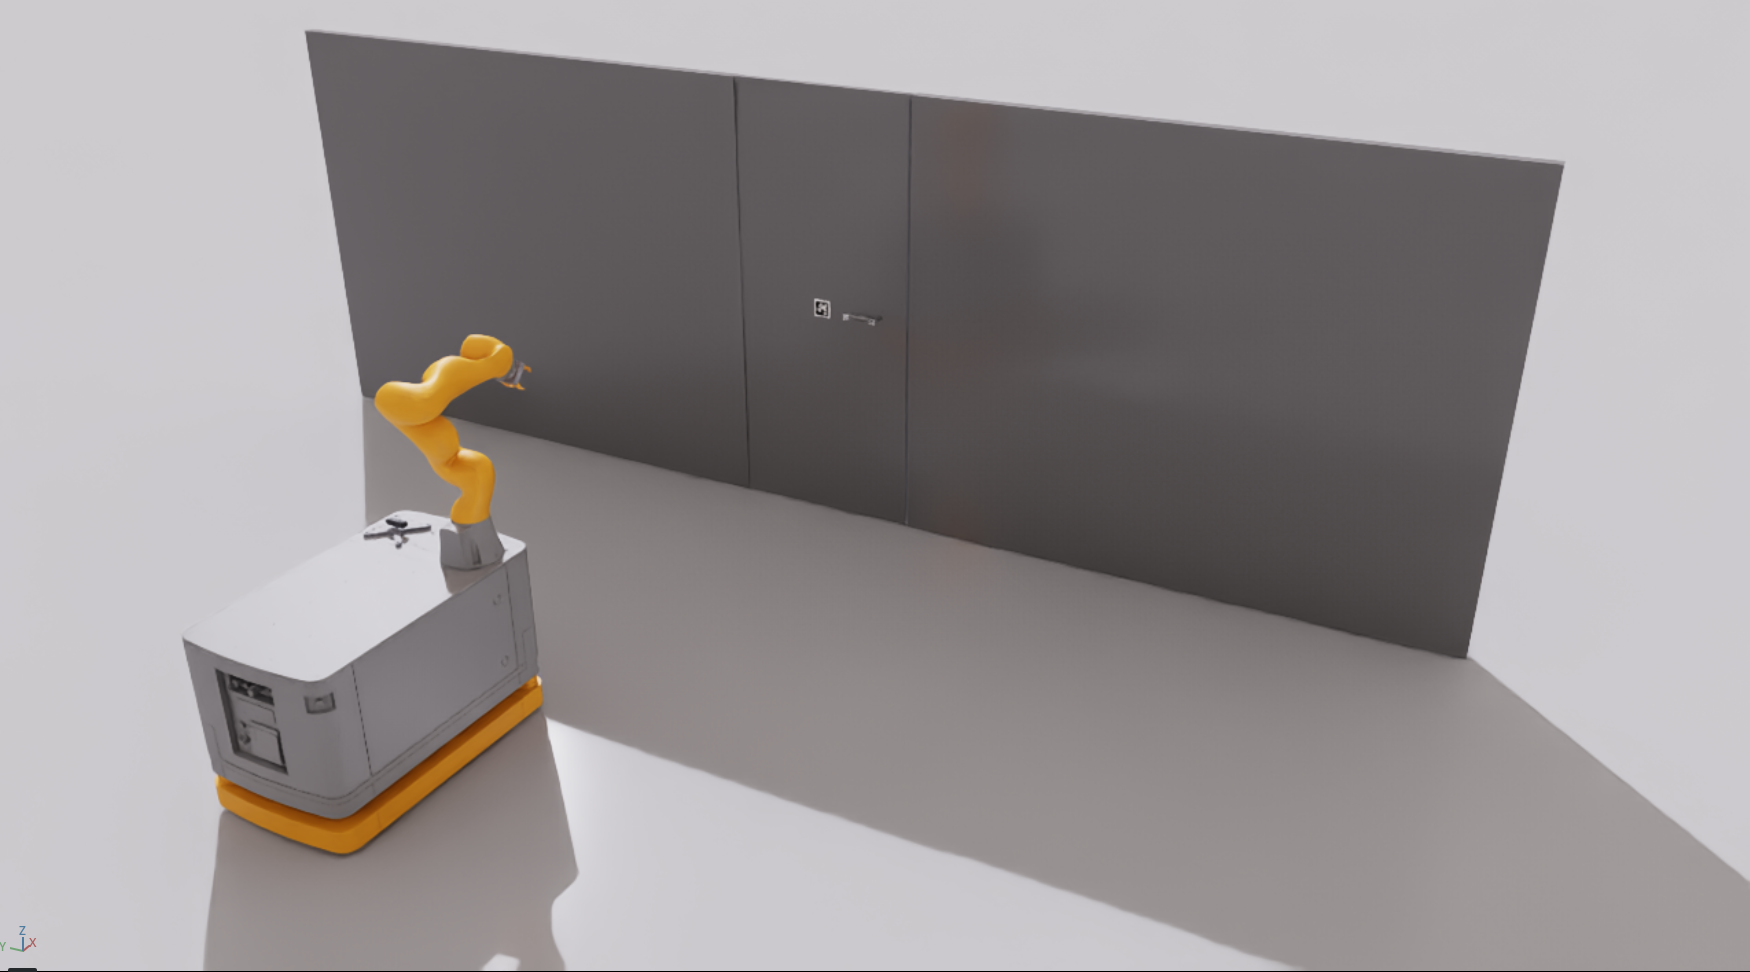
\includegraphics[width=\textwidth]{figures/kl_slike/kl_revolute_pocetak.png}
            \caption{početno stanje}
      \end{subfigure}
      \hfill
      \begin{subfigure}[b]{0.48\textwidth}
            \centering
            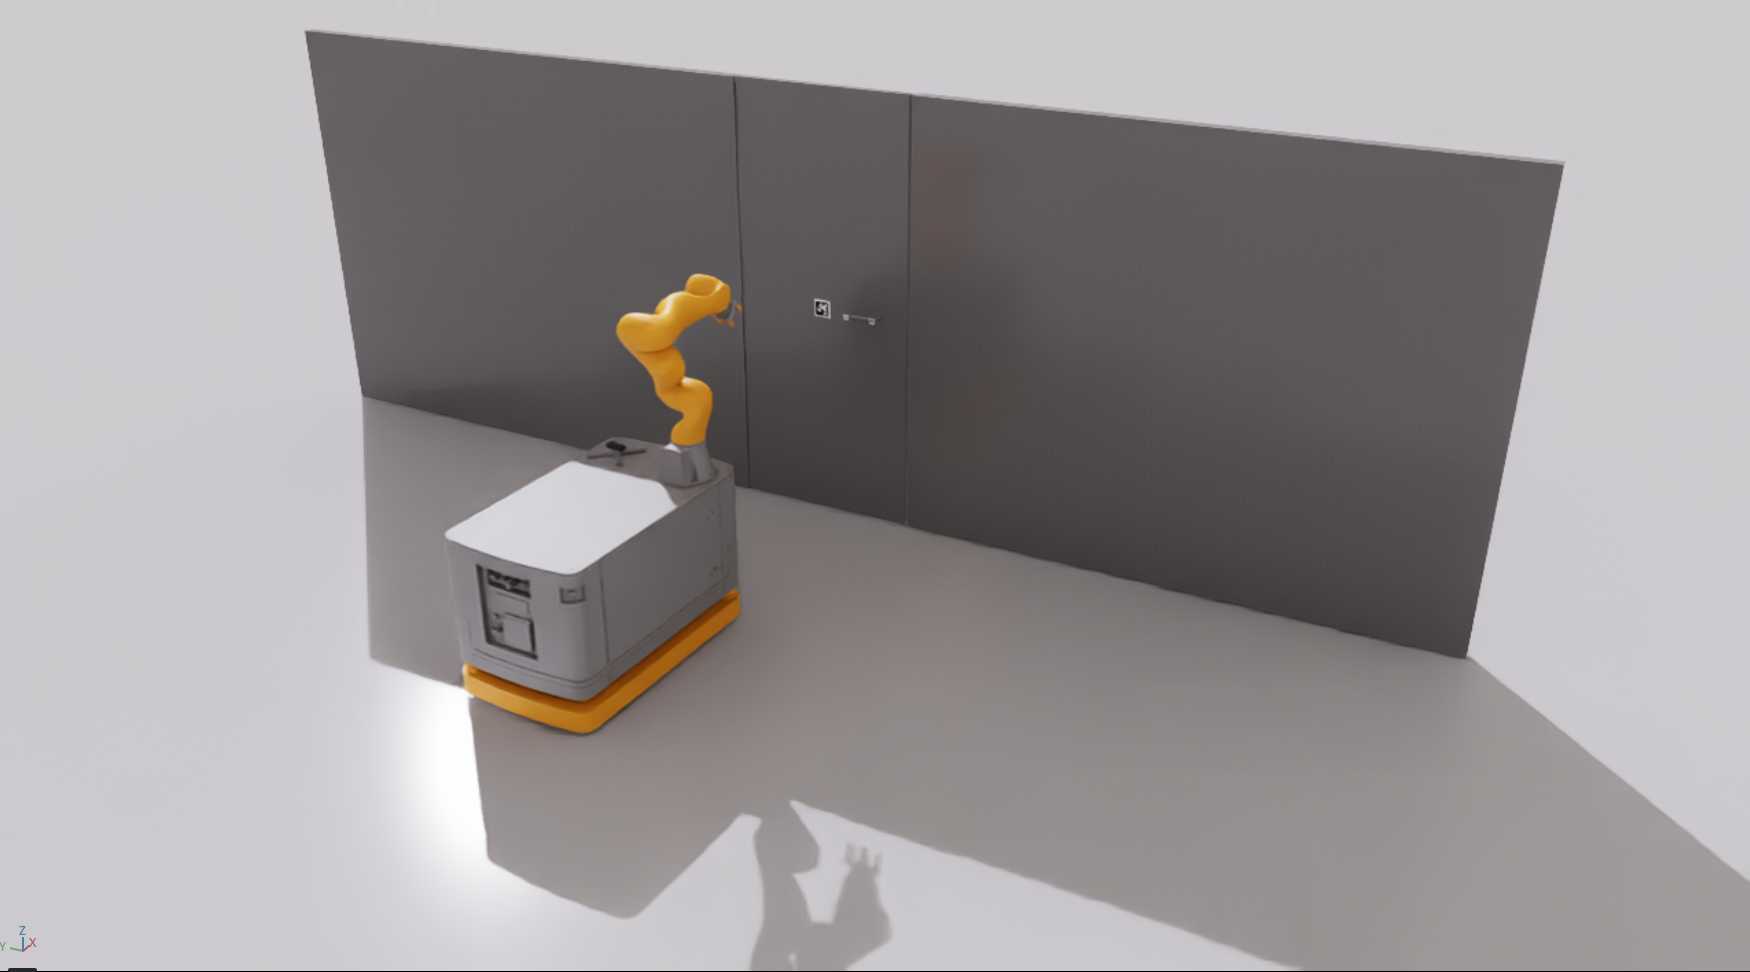
\includegraphics[width=\textwidth]{figures/kl_slike/kl_revolute_prilazak.png}
            \caption{prilazak vratima}
      \end{subfigure}

      \vspace{4pt}
      \begin{subfigure}[b]{0.48\textwidth}
            \centering
            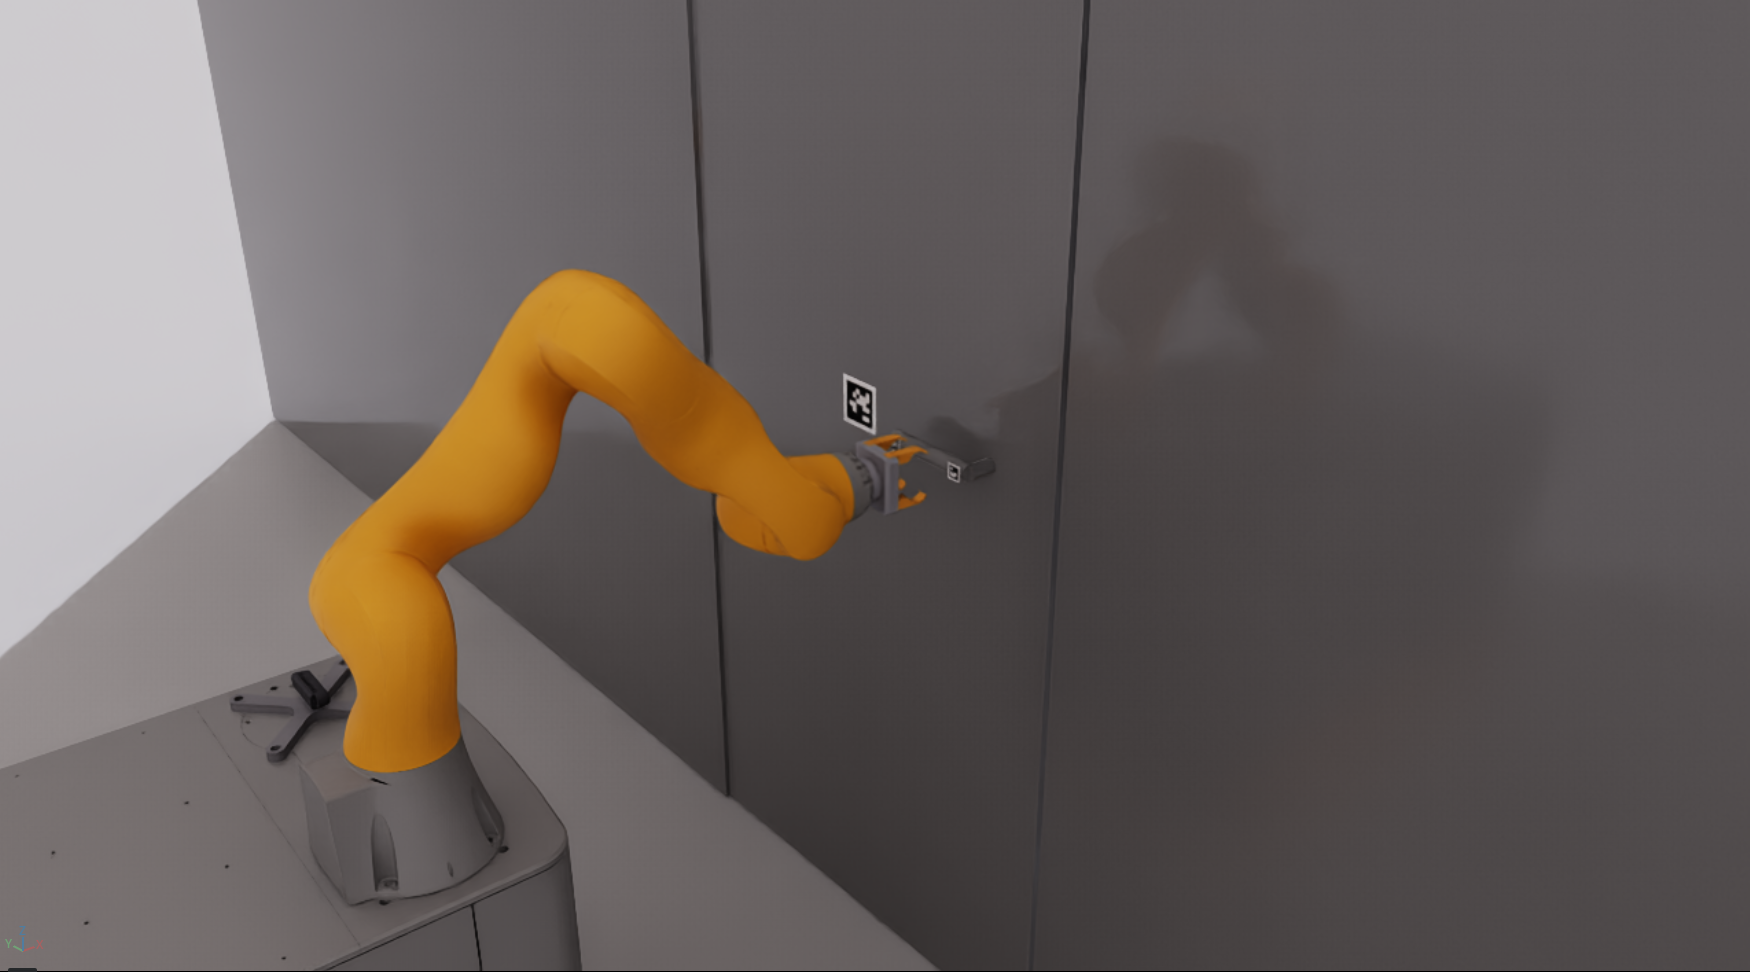
\includegraphics[width=\textwidth]{figures/kl_slike/kl_revolute_hvat.png}
            \caption{hvat kvake}
      \end{subfigure}
      \hfill
      \begin{subfigure}[b]{0.48\textwidth}
            \centering
            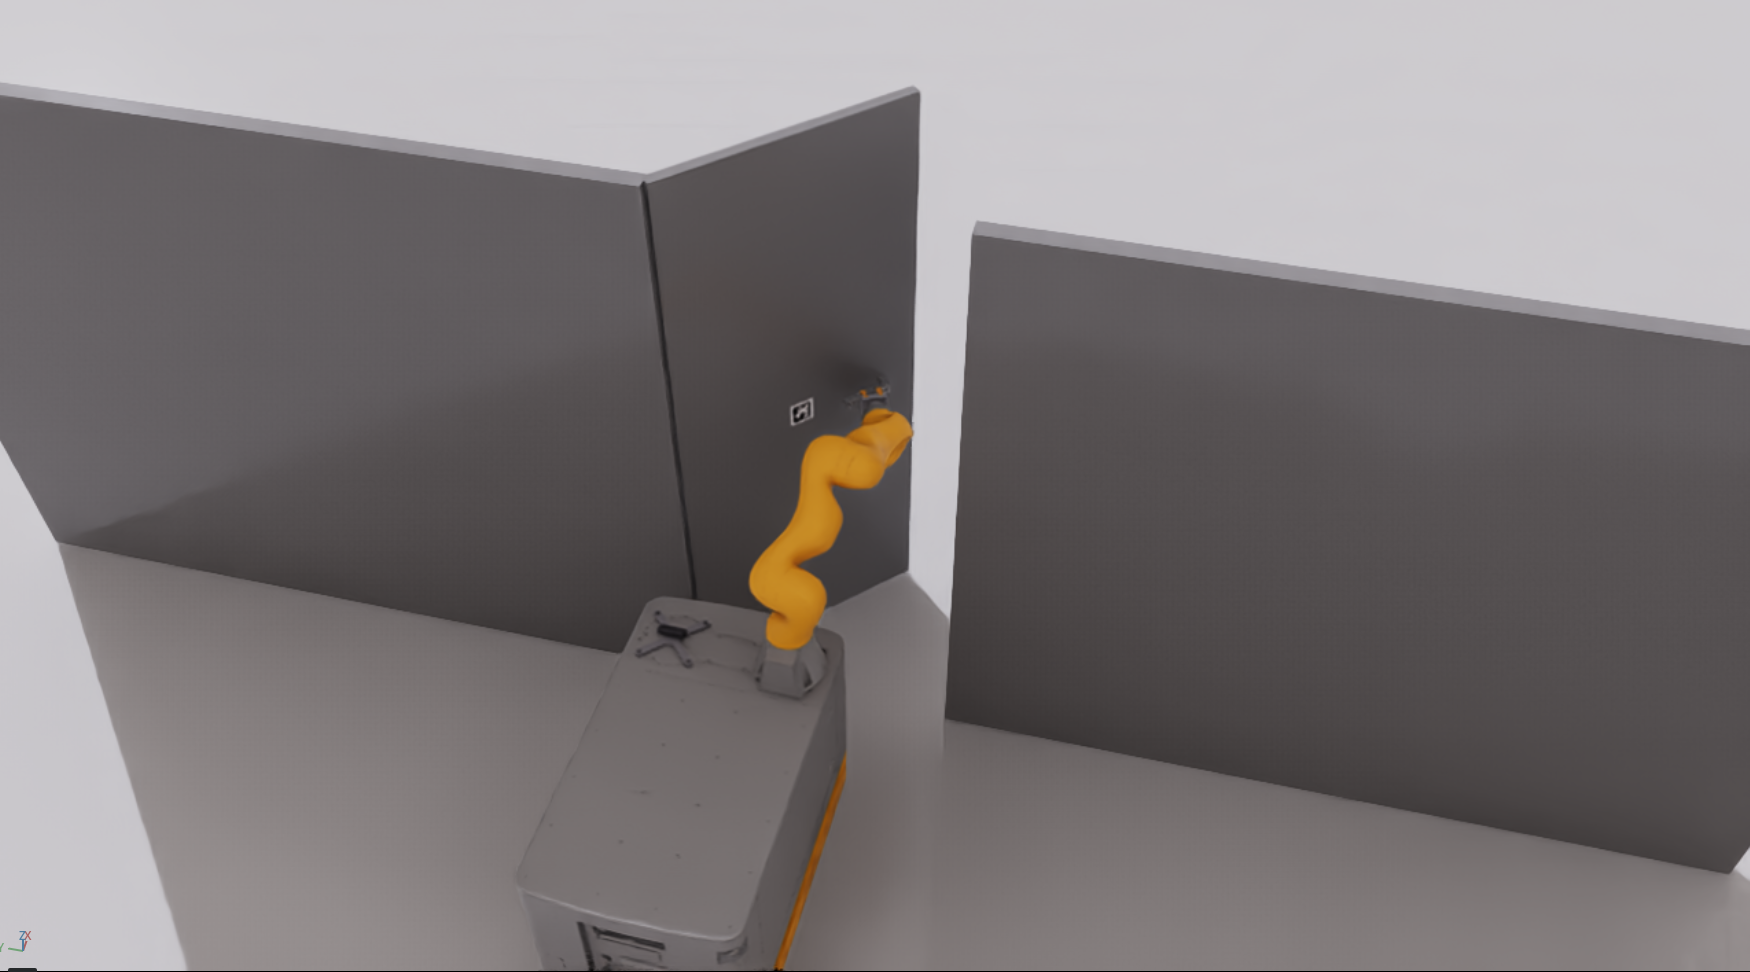
\includegraphics[width=\textwidth]{figures/kl_slike/kl_revolute_otvaranje.png}
            \caption{otvaranje}
      \end{subfigure}

      \vspace{4pt}
      \begin{subfigure}[b]{0.48\textwidth}
            \centering
            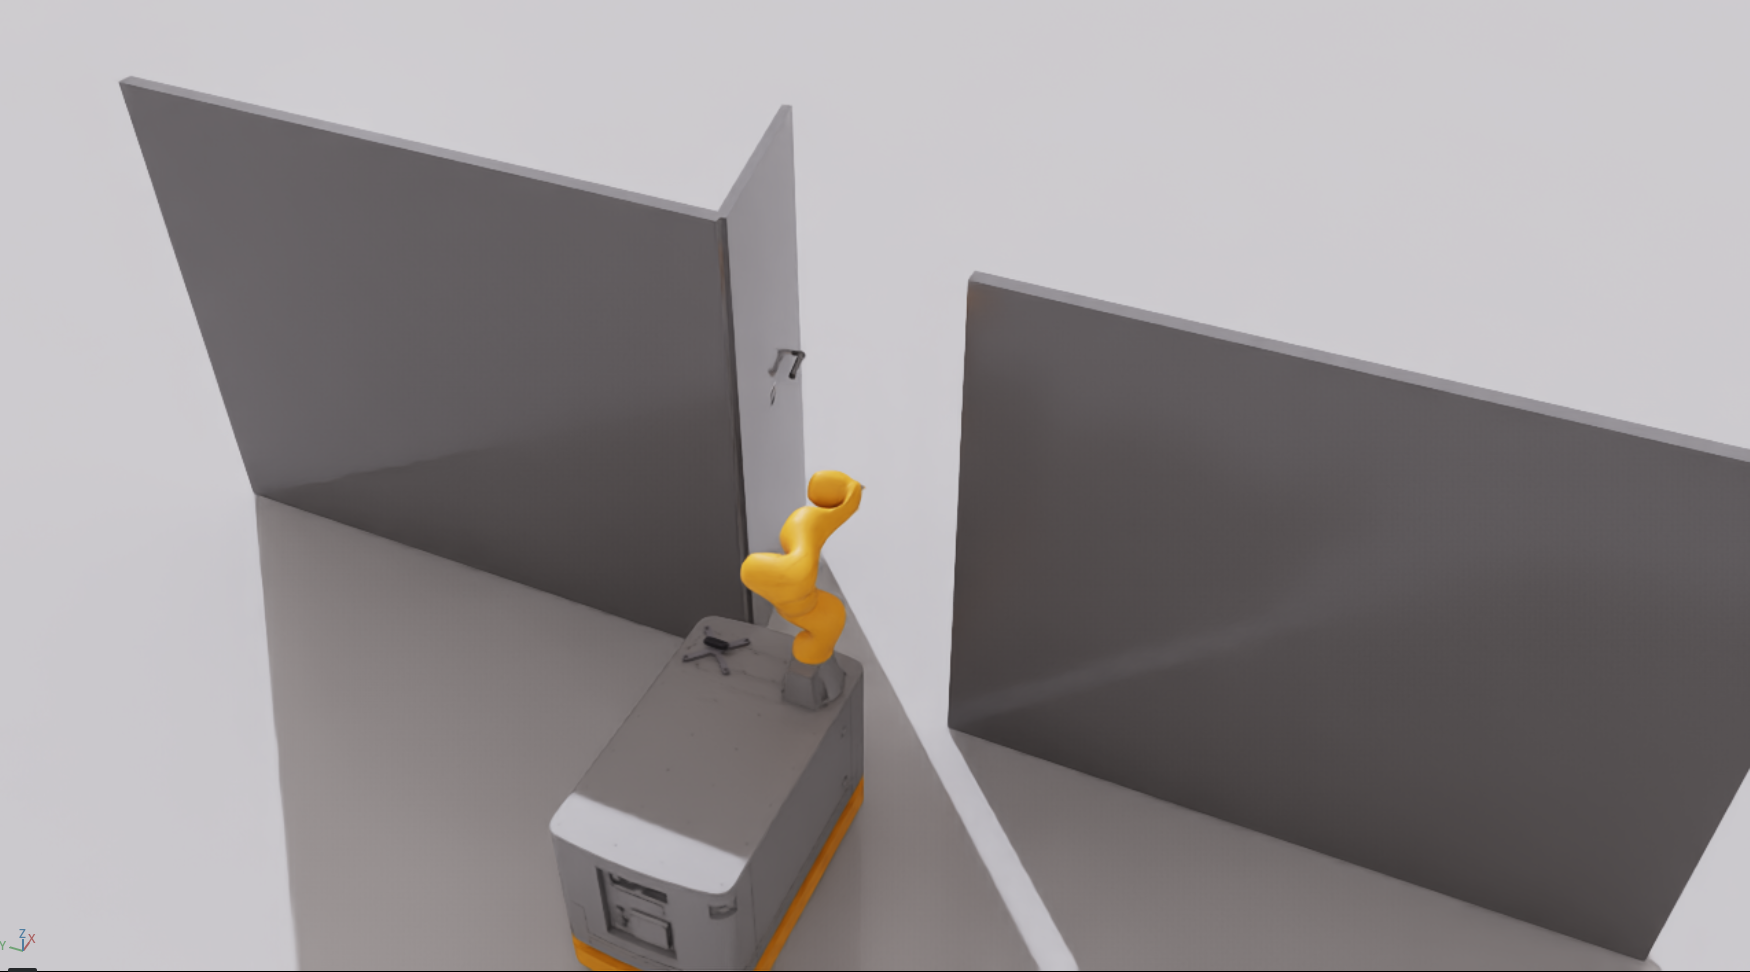
\includegraphics[width=\textwidth]{figures/kl_slike/kl_revolute_namjestanje.png}
            \caption{namještanje pred otvorom}
      \end{subfigure}
      \hfill
      \begin{subfigure}[b]{0.48\textwidth}
            \centering
            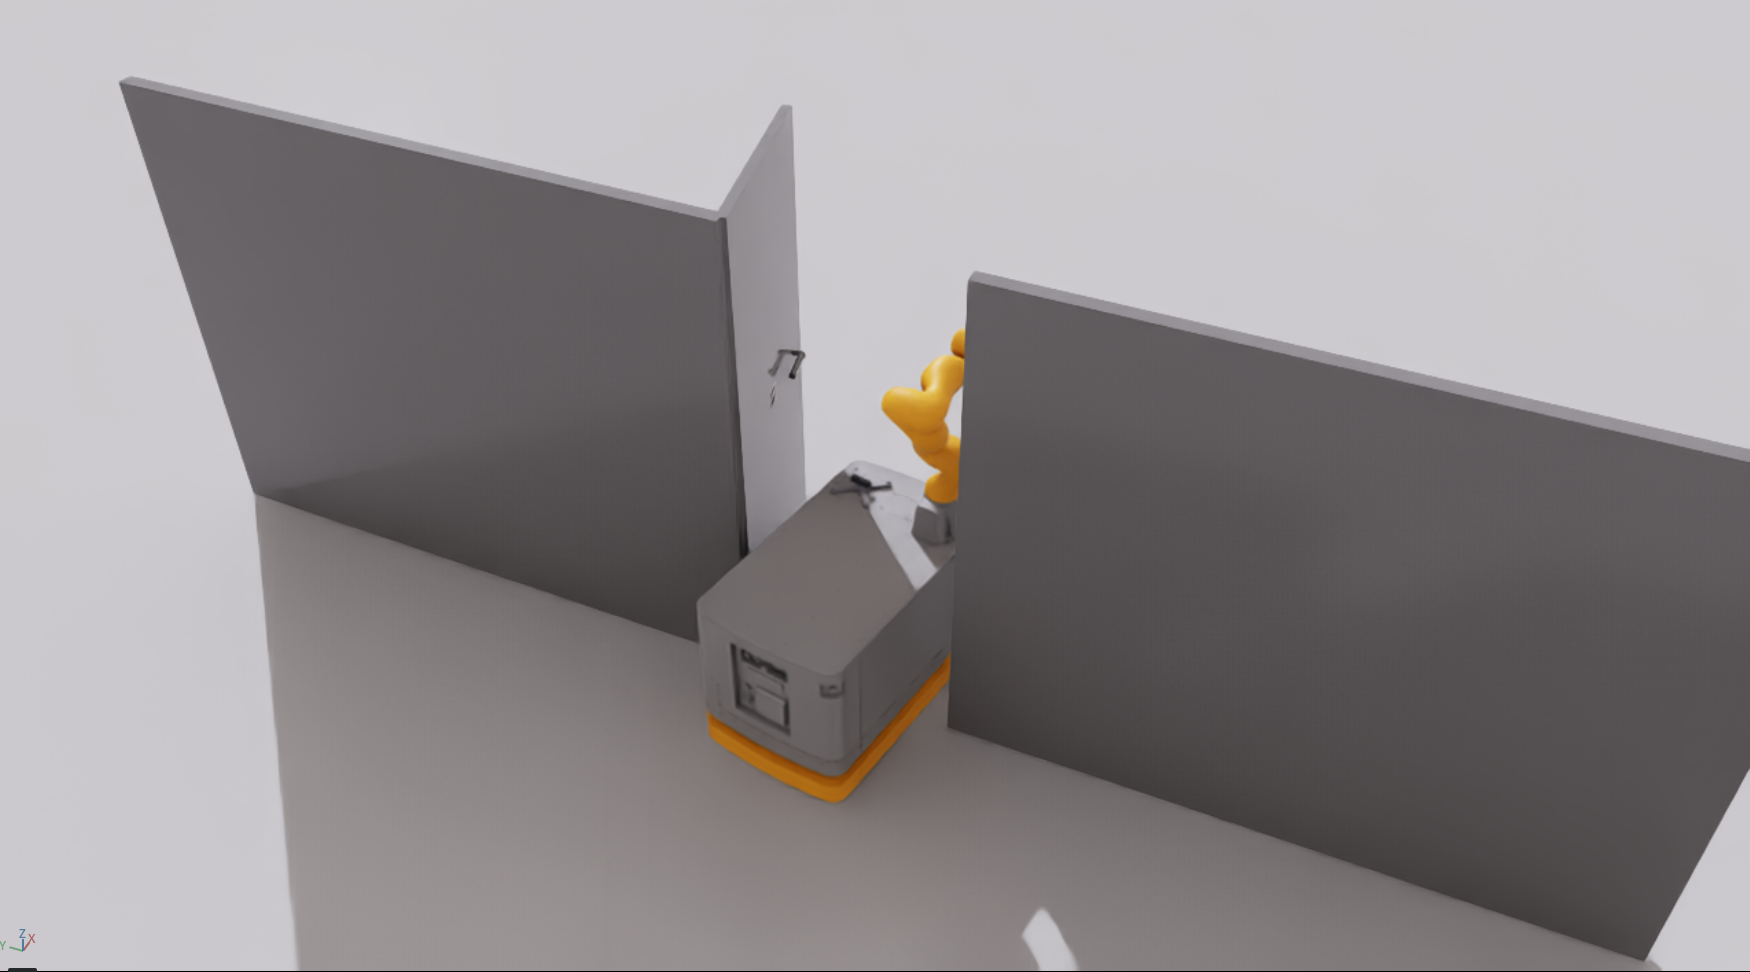
\includegraphics[width=\textwidth]{figures/kl_slike/kl_revolute_prolaz.png}
            \caption{prolazak kroz vrata}
      \end{subfigure}
      \caption{Faze izvođenja klasičnog pristupa na zakretnim vratima}
      \label{fig:faze-klasicni-zakretna}
\end{figure}

\begin{figure}[H]
      \centering
      \begin{subfigure}[b]{0.48\textwidth}
            \centering
            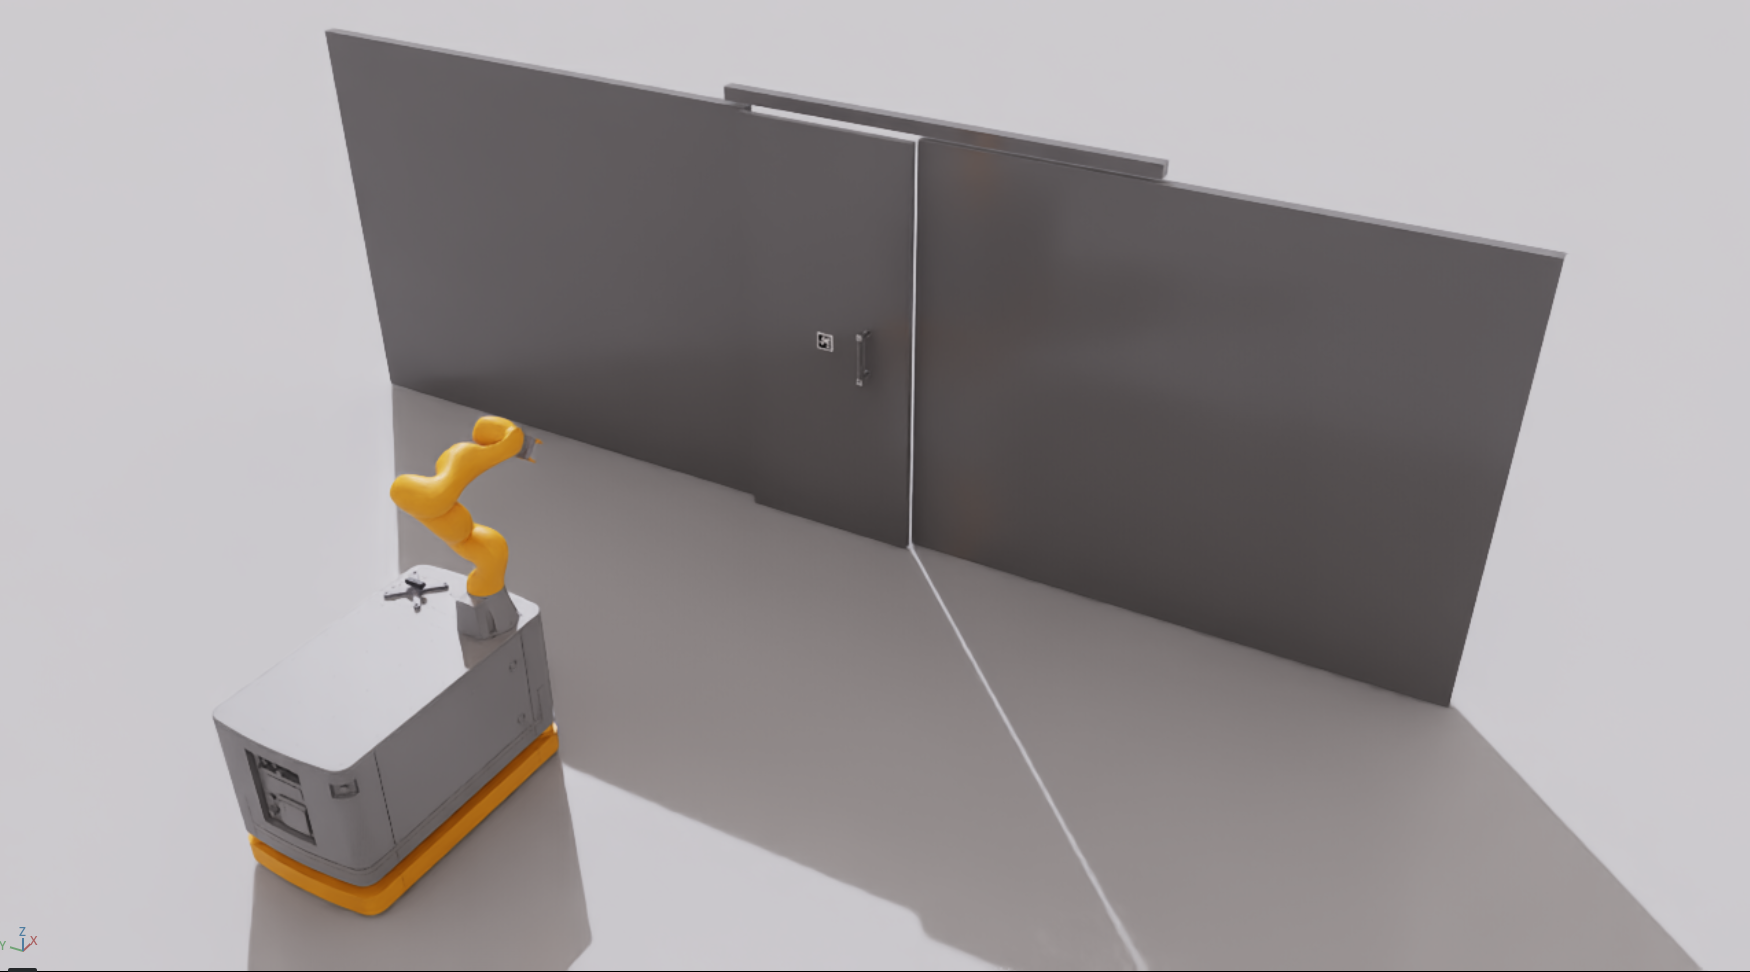
\includegraphics[width=\textwidth]{figures/kl_slike/kl_sliding_pocetak.png}
            \caption{početno stanje}
      \end{subfigure}
      \hfill
      \begin{subfigure}[b]{0.48\textwidth}
            \centering
            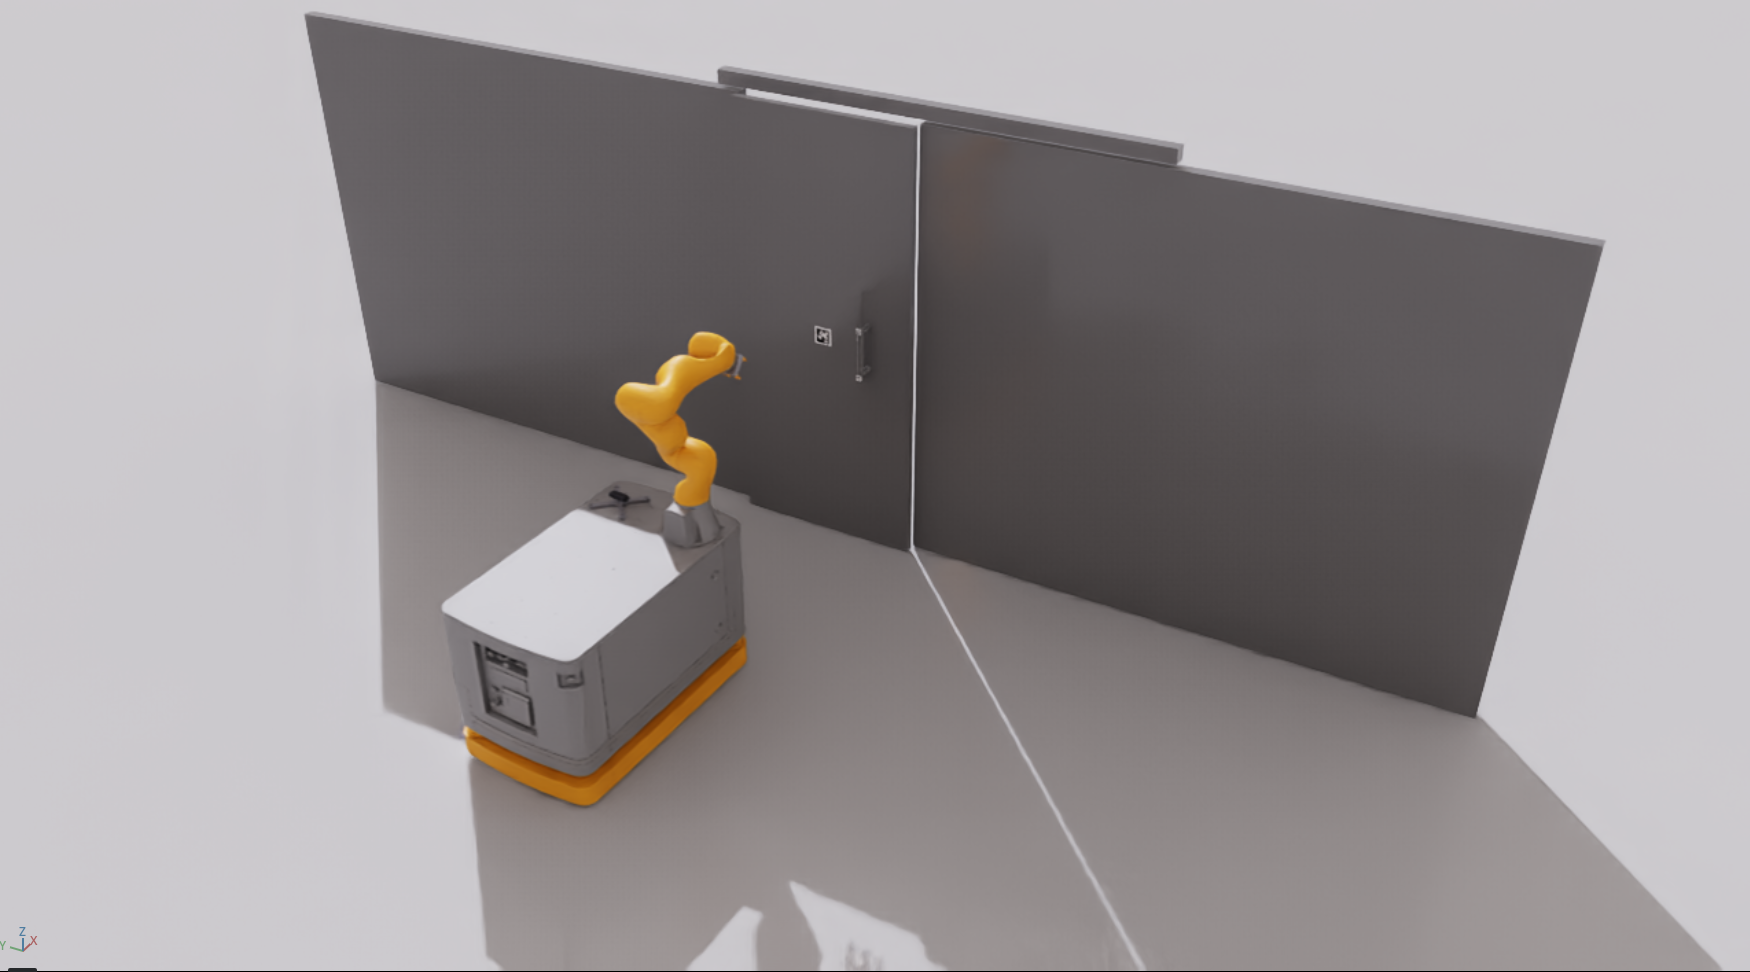
\includegraphics[width=\textwidth]{figures/kl_slike/kl_sliding_prilazak.png}
            \caption{prilazak vratima}
      \end{subfigure}

      \vspace{4pt}
      \begin{subfigure}[b]{0.48\textwidth}
            \centering
            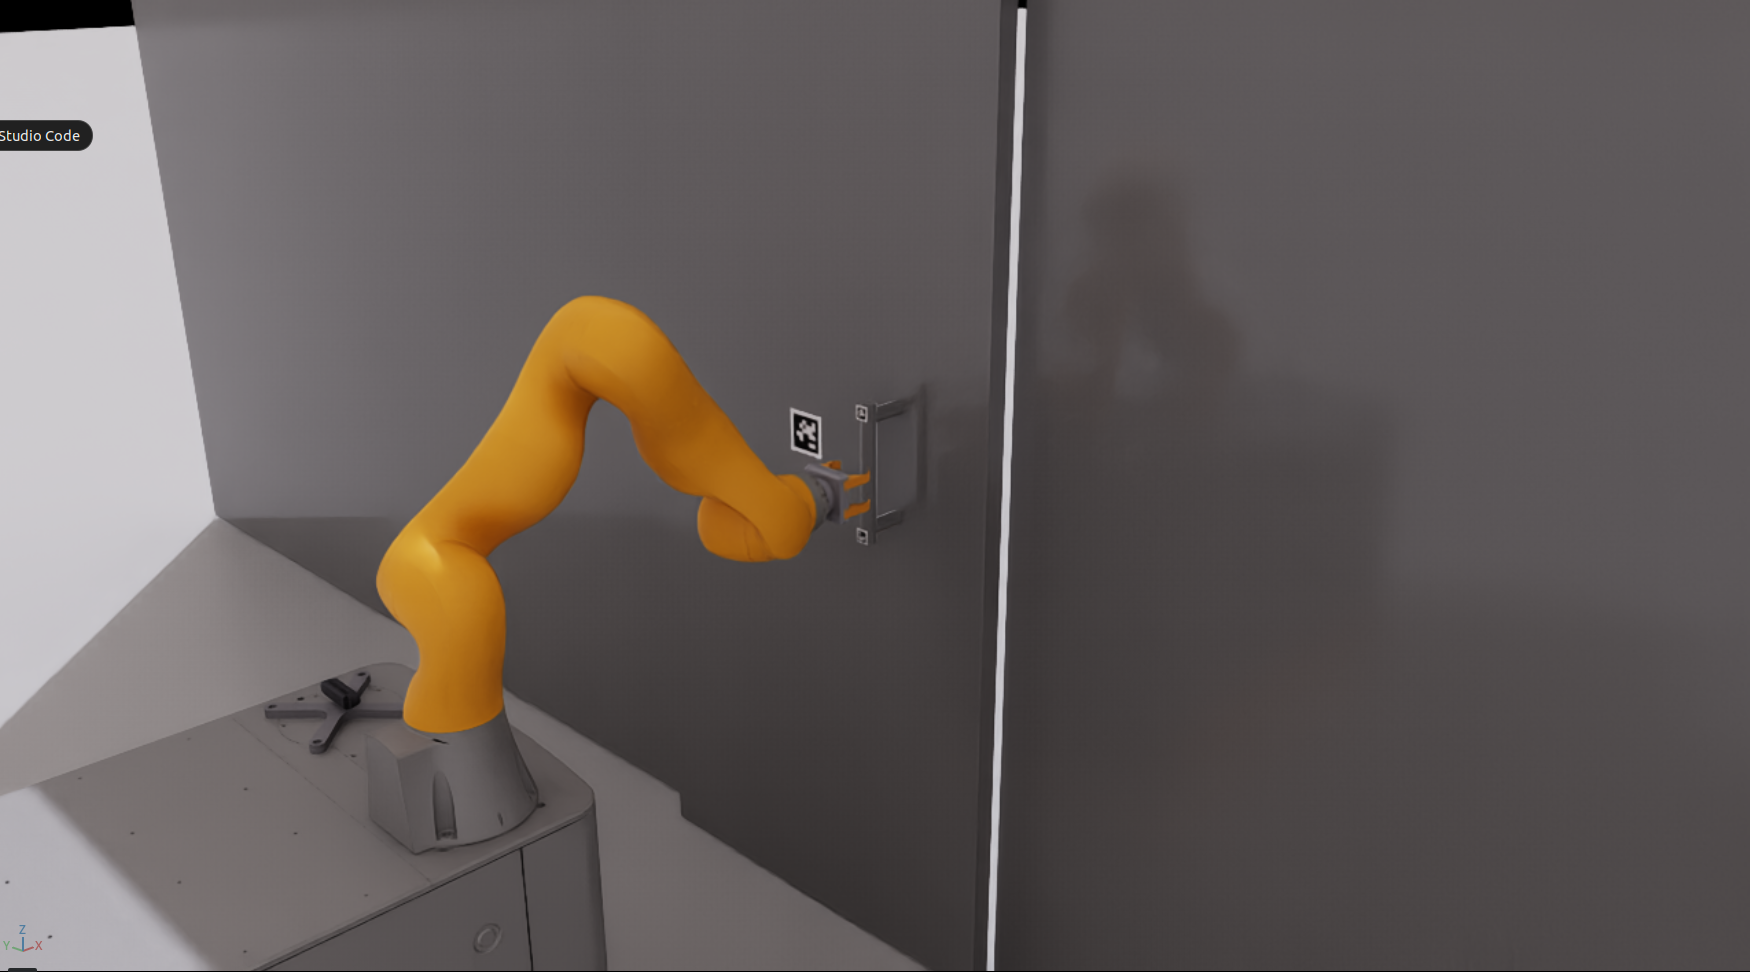
\includegraphics[width=\textwidth]{figures/kl_slike/kl_sliding_hvat.png}
            \caption{hvat kvake}
      \end{subfigure}
      \hfill
      \begin{subfigure}[b]{0.48\textwidth}
            \centering
            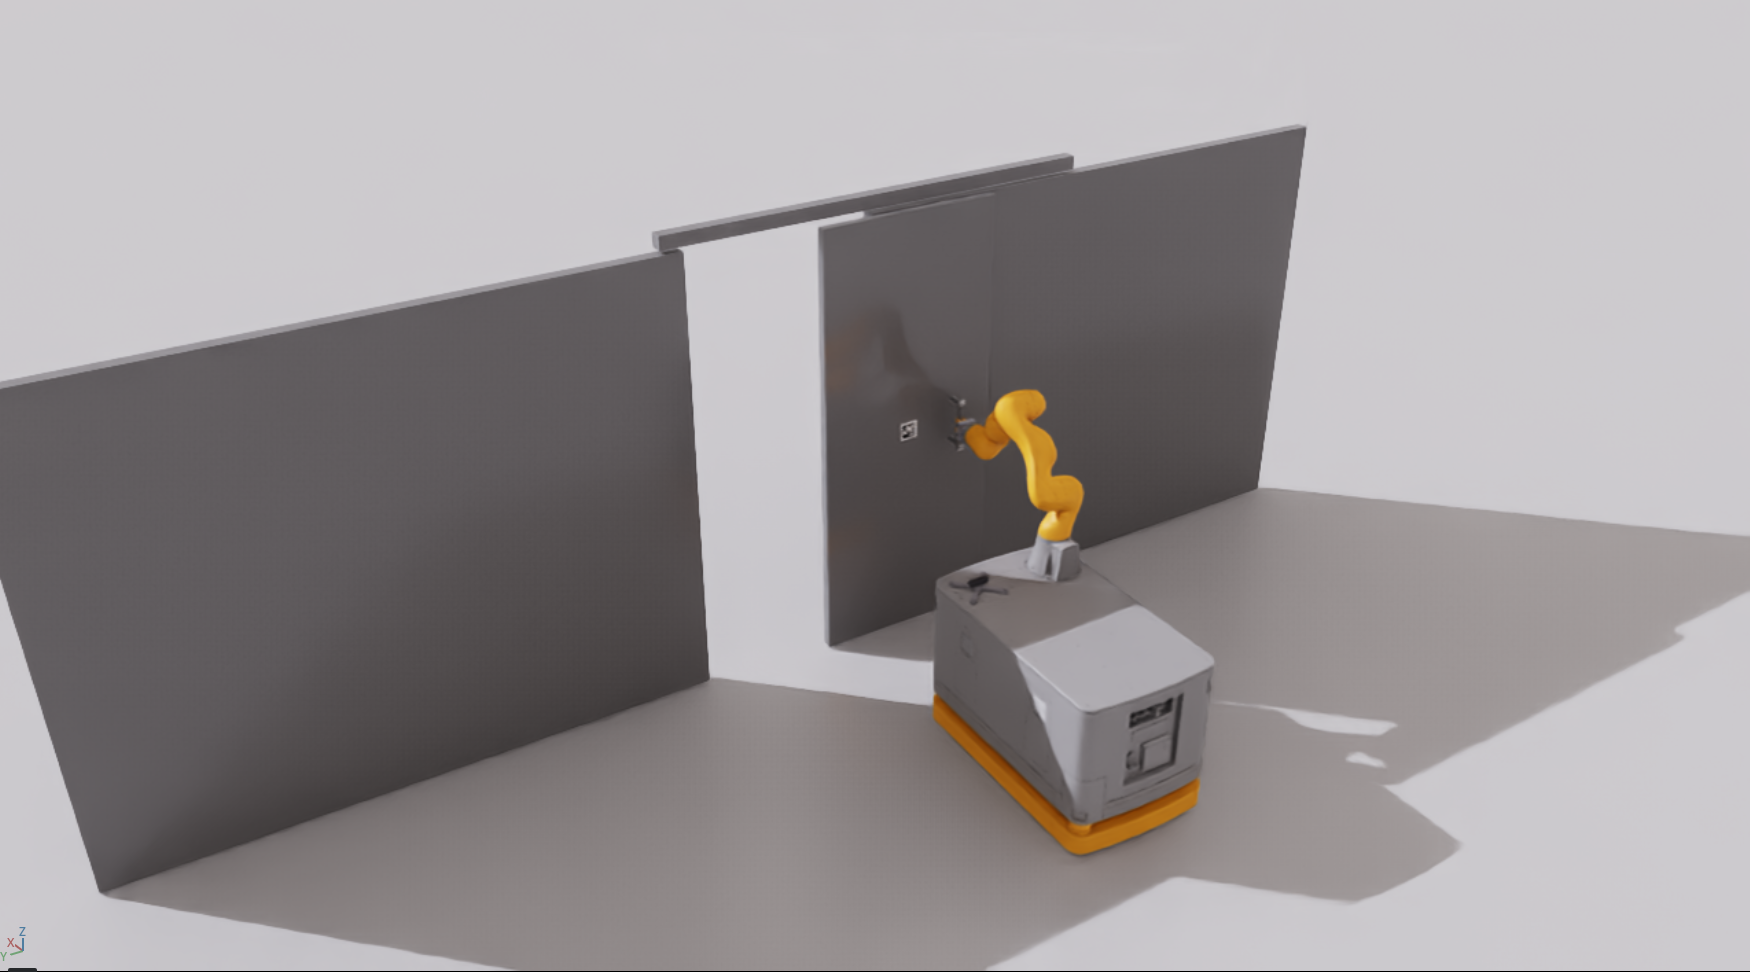
\includegraphics[width=\textwidth]{figures/kl_slike/kl_sliding_otvaranje.png}
            \caption{otvaranje}
      \end{subfigure}

      \vspace{4pt}
      \begin{subfigure}[b]{0.48\textwidth}
            \centering
            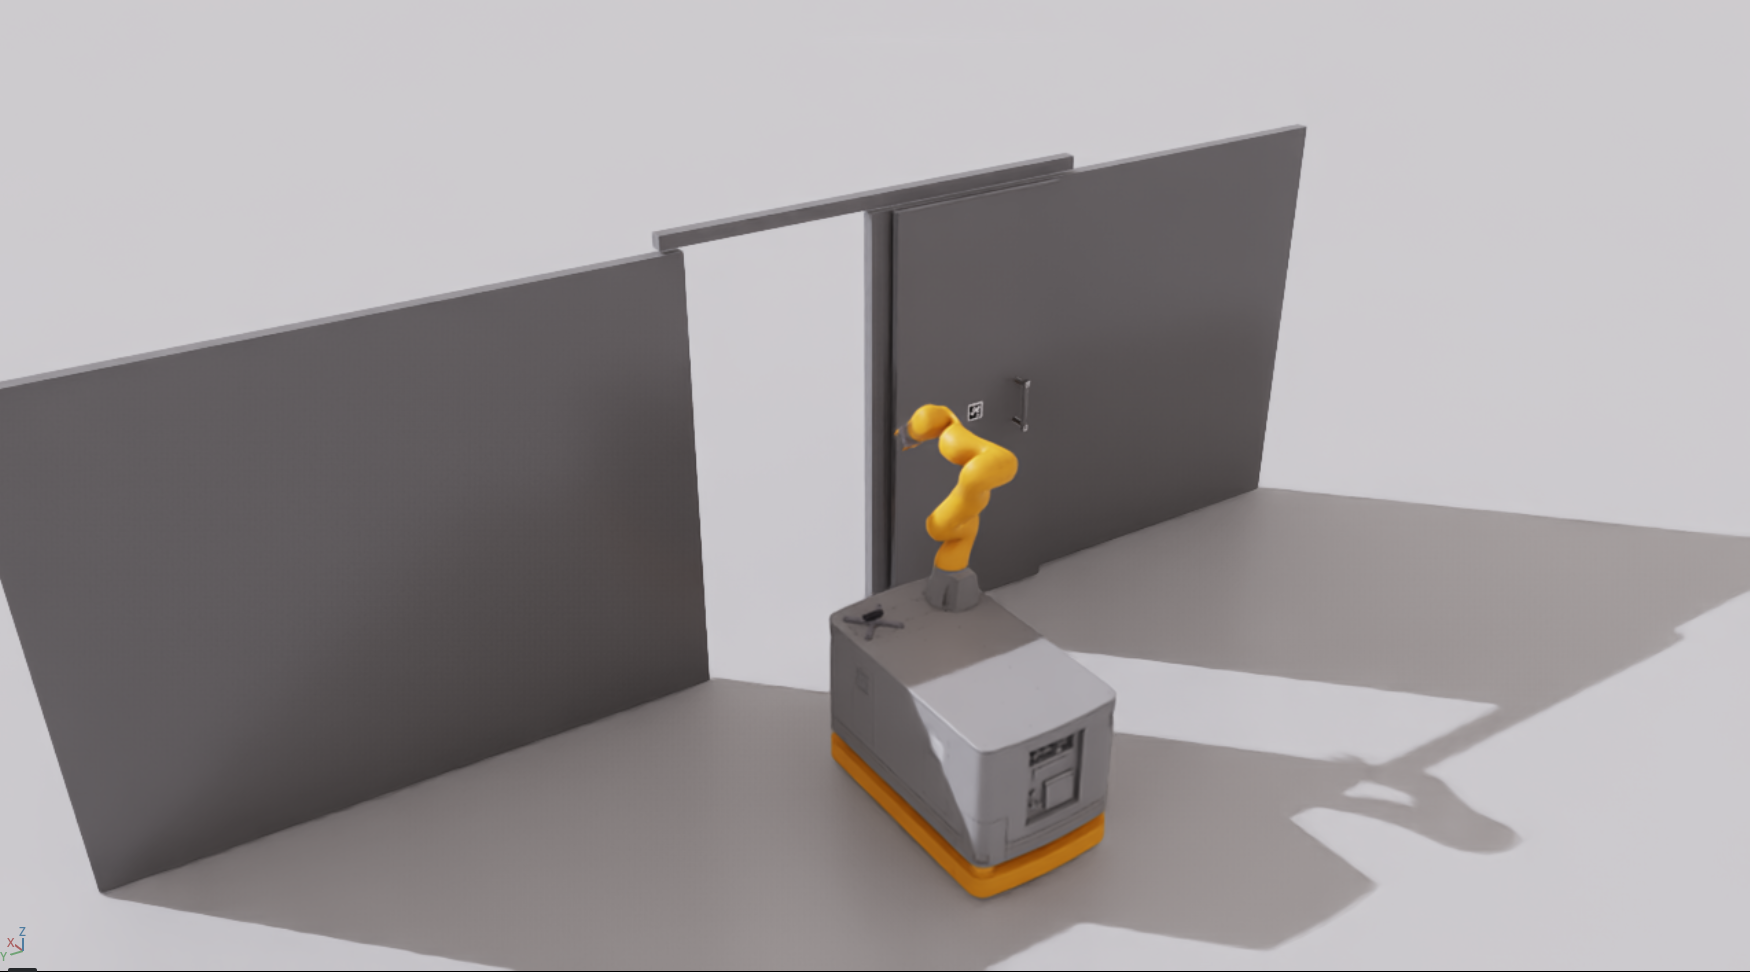
\includegraphics[width=\textwidth]{figures/kl_slike/kl_sliding_namjestanje.png}
            \caption{namještanje pred otvorom}
      \end{subfigure}
      \hfill
      \begin{subfigure}[b]{0.48\textwidth}
            \centering
            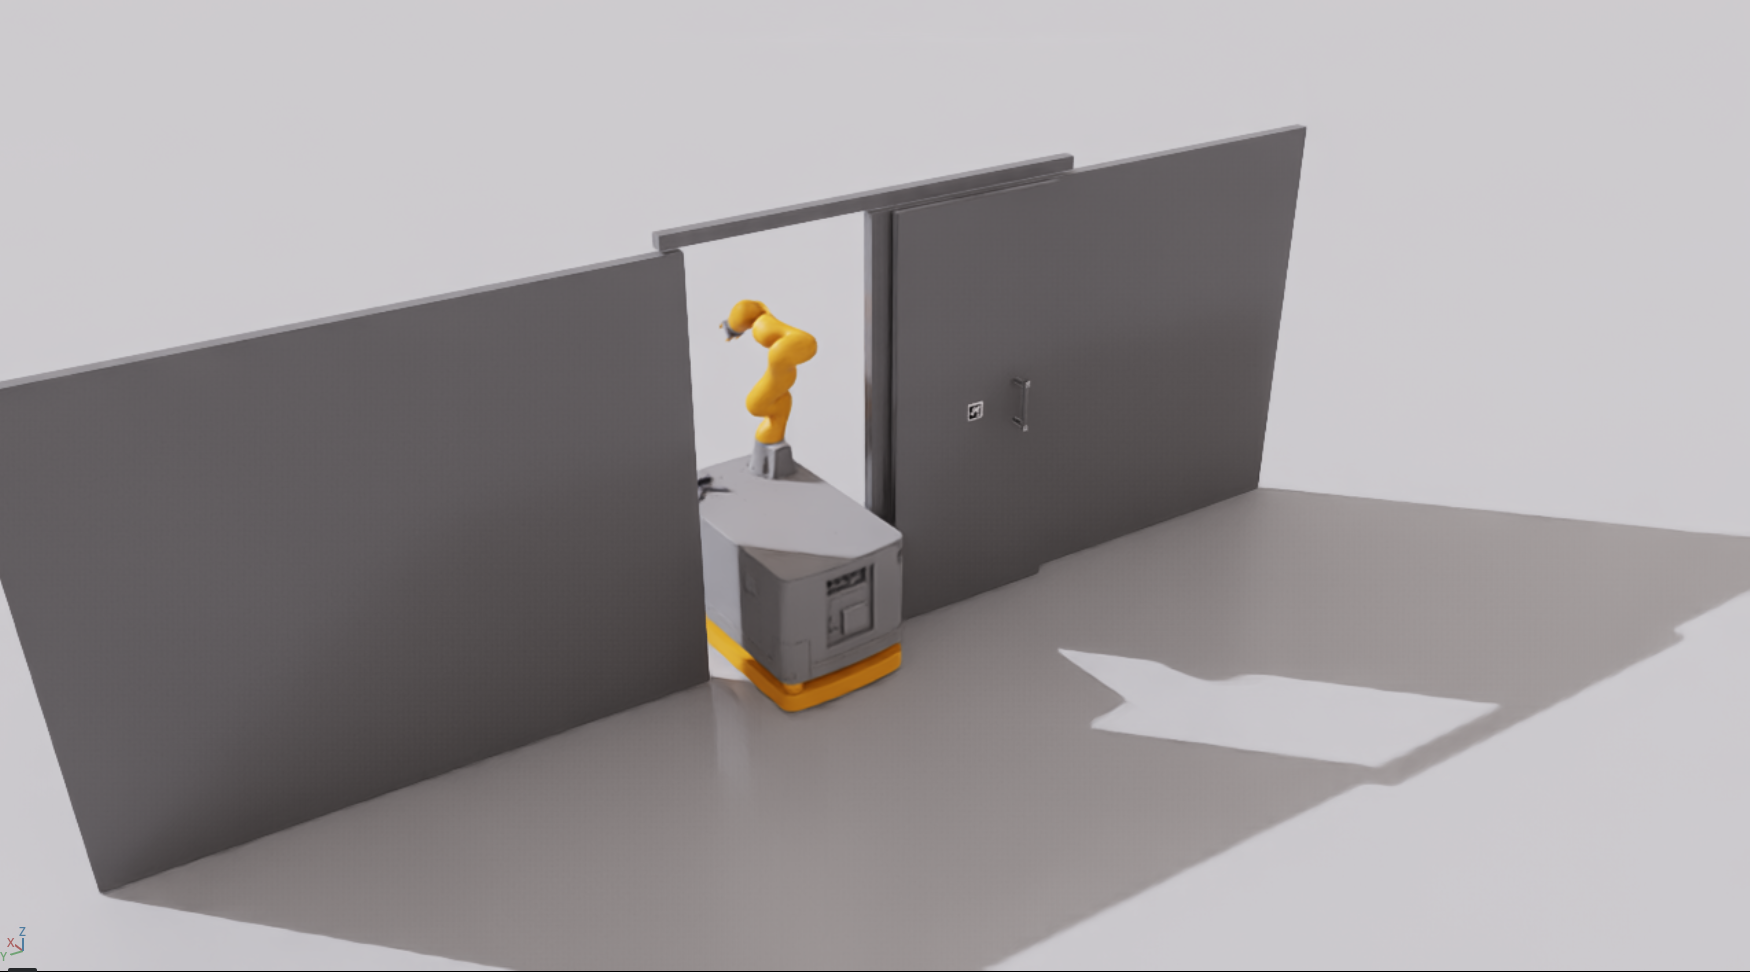
\includegraphics[width=\textwidth]{figures/kl_slike/kl_sliding_prolaz.png}
            \caption{prolazak kroz vrata}
      \end{subfigure}
      \caption{Faze izvođenja klasičnog pristupa na kliznim vratima}
      \label{fig:faze-klasicni-klizna}
\end{figure}

\subsection{Prilazak i hvat}

Pogreška poravnanja platforme iznosi 1,2 do 1,5\textdegree{}. Odstupanje postignute pred-hvatne poze od cilja
iznosi 8 do 11 mm u položaju te 0.1 do 0.2\textdegree{} u orijentaciji, a odstupanje same poze hvata 6 do
8 mm i oko 0.5\textdegree{}. Prepoznavanje tipa kvake iz geometrije (potpoglavlje \ref{sec:tip-kvake})
pokazalo se pouzdanim na objema scenama vrata.

\subsection{Zakretna vrata}

Guranje se zaustavlja na 70\textdegree{}, a završni zakret platforme
(potpoglavlje \ref{sec:zavrsni-zakret}) vrata doguruje do otprilike 100\textdegree{}, što je
dovoljno za prolazak. Izmjerene vrijednosti navedene su u tablici \ref{tab:rezultati-zakretna}.

\begin{table}[H]
      \centering
      \caption{Izmjerene vrijednosti pri otvaranju zakretnih vrata}
      \label{tab:rezultati-zakretna}
      \begin{tabular}{@{}ll@{}}
            \toprule
            Veličina                    & Vrijednost                                          \\
            \midrule
            Kut otvaranja guranjem      & 70\textdegree{} (cilj), 71\textdegree{}     stvarno \\
            Kut nakon završnog zakreta  & oko 100\textdegree{}                                \\
            Sila u hvatu, prosječna     & 320--450 N                                          \\
            Sila u hvatu, najveća       & do 630 N                                            \\
            Radijalno klizanje hvata    & do 8 mm                                             \\
            Pogreška praćenja položaja  & 0,4--2,5 mm                                         \\
            Pogreška procjene osi šarke & 5,8 mm prosječno, do 14,3 mm \ref{sec:provjera}     \\
            \bottomrule
      \end{tabular}
\end{table}

\subsection{Klizna vrata}

Ostvareno je otvaranje od 904 do 910 mm uz cilj od 900 mm, u dva prolaza, nakon čega je prolazak
kroz otvor uspješan. Sila u hvatu iznosila je u prosjeku 240 do 260 N, s vrhom do 660 N, a
klizanje hvata ostalo je između 4 i 6 mm kroz cijeli manevar. To je manje nego kod zakretnih
vrata, u skladu s time da se kod kliznih vrata smjer sile poklapa sa smjerom gibanja hvata, dok
kod zakretnih hvat prati zakrivljenu putanju. Prijeđeni put platforme iznosio je 900 mm, mjereno
odometrijom.

\section{Ograničenja}
\label{sec:klasicni-limits}

\begin{itemize}
      \item Gibanje platforme ima izraženu mrtvu zonu i ne postiže naređenu brzinu. Rotacija se
            ne pokreće ispod 0,36 rad/s, bočna translacija ispod otprilike 0,18 m/s, a uzdužna
            translacija postiže oko 45 \% naređenoga. Omjer je dosljedan kroz ispitani raspon
            brzina od 0,05 do 0,22 m/s, a brzina očitana u samom simulatoru odgovara naređenoj, pa
            je uzrok negdje u prijenosu naredbe do fizike platforme. Provjereno je i isključeno
            više mogućih uzroka: pogon i trenje u zglobu vrata, viskozno prigušenje platforme,
            brzina same simulacije te trajanje prijelazne faze na početku gibanja.
            Posljedica je da regulator koji zadaje male korekcije postaje dvopoložajan, jer je
            naredba ili ispod praga i bez učinka, ili puna.

      \item Prijeđeni put platforme ne smije se računati iz naređene brzine i vremena, iz
            prethodno navedenog razloga. Umjesto toga se mjeri odometrijom (potpoglavlje
            \ref{sec:odometrija}), pa se svi iznosi pomaka u ovom poglavlju odnose na izmjerenu,
            a ne na zadanu veličinu.

      \item Kako je navedeno u potpoglavlju \ref{sec:vrata}, zglob koji bi omogućio zakretanje
            kvake u konačnom je modelu nepomičan. Ta je odluka svjesno smanjenje opsega rada, ne
            nedostatak: zakretanje kvake bilo je u ranijoj fazi razvoja najproblematičniji dio
            zadatka, jer je kruto pozicijsko upravljanje tim dodatnim stupnjem slobode davalo
            velike kontaktne sile na svako odstupanje procjene. Uklanjanjem tog stupnja slobode
            zadatak je sveden na jedan stupanj slobode po tipu vrata. Ista je odluka primijenjena
            i u pristupu temeljenom na učenju, opisanom u poglavlju \ref{ch:rl}, čime ostaje
            osnova za usporedbu dvaju pristupa.

      \item Guranje zakretnih vrata ne prelazi otprilike 71\textdegree{}. Kako se vrata otvaraju,
            potreban doseg manipulatora raste s 0,81 na 0,88 m, a to se ne može nadoknaditi
            zakretanjem platforme, jer rotacija ima mrtvu zonu opisanu gore: svaki zakret kreće s
            barem 20\textdegree{}/s i slomi vezu između manipulatora i kvake. Ograničenje je
            zaobiđeno završnim zakretom platforme (potpoglavlje \ref{sec:zavrsni-zakret}),
            koji vrata doguruje do otprilike 100\textdegree{} bez opterećenja hvata.
            Otvaranje preko 100\textdegree{} zahtijevalo bi prepozicioniranje hvata, dakle
            puštanje kvake, premještanje platforme i ponovni hvat iz povoljnije konfiguracije, što
            nije izvedeno u opsegu ovog rada.

      \item Sustav sadrži zaseban postupak procjene geometrije ograničenja iz odnosa sile i
            gibanja, opisan u poglavlju \ref{ch:procjena}, ali on u klasičnom pristupu nije
            povezan s izvođenjem: os šarke u fazi otvaranja izračunava se geometrijski iz
            percepcije, a procjena iz gibanja postoji u zasebnim, samostalno pokretanim
            skriptama, izvan glavnog tijeka zadatka. Sustav zna i procijeniti ograničenje iz
            gibanja i otvoriti vrata, ali te dvije sposobnosti nisu spojene u jedan tijek
            izvođenja.

      \item Lidar tijekom otvaranja i prolaska prati postoji li prepreka neposredno ispred
            platforme i zaustavlja zadatak ako je udaljenost premala, ali ne raspolaže
            planiranjem puta niti izbjegavanjem prepreke.
\end{itemize}
\chapter{PRISTUP TEMELJEN NA UČENJU}
\label{ch:rl}

Pristup temeljen na učenju rješava isti zadatak kao poglavlje \ref{ch:klasicni}, ali bitno
drugačijim sredstvima. Klasični pristup vrh alata vodi krutim pozicijskim
upravljanjem po unaprijed izračunatoj putanji, uz geometriju ograničenja poznatu iz percepcije.
Ovdje se, umjesto toga, uvodi varijabilna impedancija: politika u svakom koraku sama bira koliko
će regulator biti krut po svakoj osi, a geometriju ograničenja ne dobiva ni iz percepcije ni iz
eksplicitnog procjenitelja, nego je mora otkriti iz vlastitih opažanja sile i gibanja. To je
izravan odgovor na nalaz iz poglavlja \ref{ch:klasicni}: kruto pozicijsko praćenje luka davalo je
velike kontaktne sile na svako odstupanje procjene, pa varijabilna impedancija postoji upravo
zato da politika tu krutost regulira sama.

\section{Opseg}
\label{sec:rl-opseg}

Politika ne uči prilaz ni hvat kvake. Epizoda počinje od stanja u kojem prihvatnica već drži
kvaku, a klasični postupak prilaza i hvata (potpoglavlje \ref{sec:prilaz}) smatra se zajedničkim
za oba pristupa. Razlog je dvostruk: prilaz i hvat rješavaju problem navigacije i planiranja
gibanja, a ne problem interakcije koji je predmet ovog rada, i njihovo bi dupliciranje otežalo
poštenu usporedbu, jer bi mjerena razlika između pristupa uključivala i razliku u tome tko je
bolji u navigaciji, ne samo u interakciji. Iz istog je razloga izostavljen i prolazak kroz vrata:
i on je navigacija kroz poznatu geometriju, ista kategorija kao prilaz. Ta odluka o opsegu izravno
oblikuje ono što se u poglavlju \ref{ch:rezultati} smije uspoređivati. Usporedba se odnosi
isključivo na fazu otvaranja, ne na cijeli zadatak, dok klasični pristup taj cijeli zadatak
stvarno izvodi od početka do kraja.

Sam postupak prolaska kroz vrata je implementiran i radi, uključivo za slučaj naučene politike,
ali je namjerno isključen iz rezultata radi dosljednosti opsega. Vrijedan je kao potvrda da se
naučena politika može ugraditi u isti izvršni sloj kao klasični pristup.

Trening se u cijelosti odvija unutar simulacijskog okruženja Isaac Lab, bez sustava ROS 2 u
regulacijskoj petlji. Razlog je paralelizacija: trening istovremeno pokreće više stotina
okruženja, a posredovanje kroz ROS 2 bilo bi usko grlo. Epizoda traje 10 sekundi, uz korak
upravljanja od 60 Hz (fizika 120 Hz, decimacija 2), što daje 600 koraka po epizodi.

Uspješnost politike pri determinističkom izvođenju, koje se razlikuje od učenja, mjerena je
zasebno i uspoređena s klasičnim pristupom u poglavlju \ref{ch:rezultati}.

\section{Formulacija Markovljevog procesa odlučivanja}
\label{sec:mdp}

\subsection{Prostor opažanja}
\label{sec:opazanje}

Vrijedi isto načelo kao u klasičnom pristupu: kut ili pomak zgloba vrata, dakle stvarno stanje
zadatka, nikada nije dio opažanja politike, nego se koristi isključivo u nagradi i terminaciji,
gdje je legitiman jer se računa izvan regulacijske petlje. Opažanje sadrži:

\begin{itemize}
    \item pozu vrha alata u koordinatnom sustavu platforme (položaj i orijentacija);
    \item linearnu i kutnu brzinu vrha alata, u istom koordinatnom sustavu;
    \item brzinu platforme, (linearna brzina po $x$ i $y$, kutna brzina oko $z$);
    \item procijenjenu silu i moment na vrhu alata, uz Gaussov šum standardne devijacije
          0.5 N, koji odgovara šumu stvarnog procjenitelja iz poglavlja \ref{ch:procjena};
    \item vektore od platforme do najbližih točaka susjednih prepreka (zid, dovratnik), uz
          Gaussov šum standardne devijacije 1 cm, koji odgovara izmjerenoj stabilnosti sredine
          otvora iz skena lidara u klasičnom pristupu (potpoglavlje \ref{sec:prolazak});
    \item posljednju akciju.
\end{itemize}

\subsection{Prostor akcija}
\label{sec:akcije}

Ruka se upravlja regulatorom u operacijskom prostoru s varijabilnom impedancijom. Akcija zadaje
pomak reference vrha alata u odnosu na trenutnu pozu, za svih šest stupnjeva slobode, i šest
pripadnih krutosti, po jedna za svaku os. Time politika izravno bira, u svakom koraku i za
svaku os zasebno, koliko će regulator biti krut, točno ono što je poglavlje
\ref{ch:klasicni} pokazalo da kruto pozicijsko upravljanje ne može samo po sebi ostvariti.

Sam pomak reference po koraku ograničen je na 15 mm. Pri većoj vrijednosti, istraživačko ponašanje
na početku učenja trgalo je hvat sa šipke prije nego što bi politika uopće stigla nešto naučiti.

Uz šest stupnjeva slobode ruke, akcija sadrži i tri komponente brzine platforme (uzdužnu,
poprečnu i kutnu) pa politika sama koordinira ruku i platformu.

\subsection{Koordinacija platforme i manipulatora}
\label{sec:baza-uci}

Uvedena je dodatna kazna na odstupanja platforme od okomice na
ravninu vrata, s težinom razmjernom tome koliko takvo odstupanje kod danog tipa vrata stvarno
šteti: znatno većom kod zakretnih, gdje dijagonalan položaj platforme kasnije ne prolazi kroz
suženi otvor, nego kod kliznih, gdje platforma svejedno mora pratiti krilo poprečno pa okomitost
manje košta. Kazna je uz to zatvorena ovisno o ostvarenom napretku, tako da ne djeluje u ranoj
fazi zadatka, kada bi se sukobila s potrebom da politika zakrene platformu radi dosega. Ruka
je montirana izvan osi platforme, pa zakret platforme proširuje radni prostor ruke na legitiman način.

\subsection{Funkcija nagrade}
\label{sec:nagrada}

Tablica \ref{tab:nagrada} navodi sve članove nagrade. Sve su težine kalibrirane mjerenjem, ne
pogođene: cilj je bio da svaki član, u konvergiranom pokretanju, iznosi između 3 i 10 \% udjela
glavnog člana napretka, a postupak je bio pustiti probno pokretanje, očitati udjele i skalirati
težinu razmjerno odstupanju od tog cilja.

\begin{table}[H]
    \centering
    \caption{Članovi funkcije nagrade}
    \label{tab:nagrada}
    \begin{tabular}{@{}llp{0.5\textwidth}@{}}
        \toprule
        Član                 & Težina                                 & Svrha                                                   \\
        \midrule
        napredak             & $+10{,}0$                              & glavni član, normiran na prag uspjeha                   \\
        okomita sila         & $-0{,}02$                              & kazni silu okomitu na stvarni smjer gibanja vrata       \\
        zasićenje zglobova   & $-2{,}0$ (klizna), $-6{,}0$ (zakretna) & kazni rad blizu granice
        raspona zglobova ruke                                                                                                   \\
        singularitet         & $-20{,}0$                              & kazni pad manipulabilnosti ispod praga                  \\
        ubrzanje ruke        & $-5\times 10^{-4}$                     & kazni ubrzanje zglobova ruke                            \\
        trzaj ruke           & $-1\times 10^{-7}$                     & kazni trzaj (drugu derivaciju brzine) zglobova ruke     \\
        prekomjerna sila     & $-0{,}05$                              & kazni ukupnu silu iznad referentne granice              \\
        poravnanje hvata     & $-3{,}0$                               & kazni odstupanje prilazne osi hvata od okomice na krilo \\
        poravnanje platforme & $-6{,}0$ (zakretna), $-0{,}1$ (klizna) & kazni odstupanje
        platforme od okomice na ravninu vrata                                                                                   \\
        prodor u krilo       & $-20{,}0$                              & kazni približavanje ruba platforme krilu ispod
        sigurnog razmaka                                                                                                        \\
        prodor u zid         & $-20{,}0$                              & kazni približavanje ruba platforme zidu ili dovratniku
        ispod sigurnog razmaka                                                                                                  \\
        promjena akcije      & $-0{,}002$                             & kazni razliku uzastopnih akcija                         \\
        uspjeh               & $+2{,}0$                               & bonus po koraku dok je pomak vrata iznad praga uspjeha  \\
        \bottomrule
    \end{tabular}
\end{table}

Napredak se ne normira na puni hod zgloba vrata, već na puno manju referentnu vrijednost
0.6 m kod kliznih i 0.5 rad (28.6 \textdegree) kod zakretnih vrata. Uz normiranje na puni hod,
manji pomak nosio bi premalu nagradu da nadjača kazne, pa bi politika naučila dovesti vrata na
određeni pomak i ne pomicati ih dalje. Time napredak nije ograničen odozgo, već smije prijeći jedinicu,
što znači da nagrada za napredak raste što su vrata više otvorena.

Prag uspjeha, koji određuje kada se dodjeljuje bonus iz zadnjeg retka tablice \ref{tab:nagrada},
zasebna je veličina. Kod kliznih vrata poklapa se s referentnom vrijednošću normalizacije i iznosi
0.6 m. Kod zakretnih vrata je namjerno odvojen i postavljen na 1.57 rad (90 \textdegree).
Razlog je taj što je 0.5 rad dovoljno da se vrata mjerljivo pomaknu, ali nije dovoljno da
robot kroz njih prođe. Normalizacija je pritom ostala nepromijenjena kako bi kalibracija
svih ostalih veličina ostala valjana. Bonus za uspjeh dodjeljuje se po koraku dok je pomak
iznad praga, a ne kao jednokratna nagrada uz prekid epizode.

Kazna na singularitet koristi Yoshikawin indeks manipulabilnosti \cite{yoshikawa1985manipulability}:

\begin{equation}
    w(\bm{q}) = \sqrt{\det\left( \bm{J}(\bm{q}) \bm{J}(\bm{q})\transp \right)} ,
    \label{eq:manip}
\end{equation}

koji je jednak nuli točno na kinematičkom singularitetu i nigdje drugdje. Kazna je normirana na
raspon od nule do jedan.

\subsection{Terminacije}
\label{sec:terminacije}

Epizoda prekida prije isteka vremena u četiri slučaja

\begin{itemize}
    \item sila je prešla sigurnosnu granicu,
    \item hvat je izgubljen jer se vrh alata previše udaljio od šipke kvake,
    \item rub platforme je dotaknuo krilo vrata,
    \item rub platforme dotaknuo zid ili dovratnik.
\end{itemize}

\subsection{Nasumičnost pri resetu i kurikulum otpora}
\label{sec:randomizacija}

Pri svakom resetu, kut prilaska platforme vrtnji se nasumično zakreće unutar $\pm$ 20\textdegree{}
oko nazivne vrijednosti. Otpor vrata randomizira se u rasponima navedenima u poglavlju
\ref{ch:sustav} (tablica \ref{tab:randomizacija}).

Kod kliznih vrata otpor se uz to uvodi postupno, kurikulumom koji tijekom prvih 1500 iteracija
učenja linearno širi gornju granicu trenja i prigušenja s vrijednosti koja odgovara laganim
vratima do pune vrijednosti iz tablice \ref{tab:randomizacija}, nakon čega ostaje na punoj
vrijednosti do kraja treninga. Kurikulum politici omogućuje da najprije nauči na lakšim vratima, gdje
se povratna informacija o napretku redovito javlja, prije nego što se suoči s punim rasponom.
Zakretna vrata kurikulum nemaju, jer je njihov otpor za red veličine manji i politika na njemu
uči bez poteškoća; različit režim treninga po tipu vrata posljedica je te razlike u težini
zadatka, ne proizvoljne odluke.

\section{Postupak učenja}
\label{sec:trening}

Učenje se provodi algoritmom proksimalne optimizacije politike (PPO) \cite{schulman2017ppo}, s
hiperparametrima u tablici \ref{tab:ppo}.

PPO pripada familiji postupaka s aktorom i kritikom, koji uče dvije odvojene neuronske mreže.
Aktor je sama politika, ona iz opažanja daje srednje vrijednosti normalne razdiobe iz koje se potom
uzorkuje akcija, po jednu za svaku dimenziju akcijskog prostora. Kritik ničim ne upravlja, nego
iz opažanja procjenjuje očekivani ukupni diskontirani povrat iz
zatečenog stanja, dakle mjeru toga koliko je stanje samo po sebi povoljno. Kritik je potreban
jer ostvarena nagrada sama po sebi ne govori je li akcija bila dobra: visoka nagrada može biti
posljedica povoljnog stanja, a ne odabrane akcije. Razlika između stvarno ostvarenog povrata i
kritikove procjene, tzv. prednost, ono je što ulazi u ažuriranje aktora. Pozitivna
prednost pojačava vjerojatnost odabrane akcije, negativna je smanjuje. Diskontni faktor $\gamma$
i faktor generalizirane procjene prednosti $\lambda$ iz tablice \ref{tab:ppo} upravljaju upravo
izračunom te prednosti.

Obje su mreže potpuno povezane i međusobno neovisne, bez zajedničkih slojeva, s trima skrivenim
slojevima širine 256, 128 i 64. Aktor preslikava 41 ulaznu veličinu, koliko ih ima opažanje iz
potpoglavlja \ref{sec:opazanje}, u 15 izlaznih, koliko ih ima akcija iz potpoglavlja
\ref{sec:akcije}. Kritik ima isti ulaz, ali jedan jedini izlaz. Postupno suženje slojeva
uobičajen je obrazac: široki prvi sloj izdvaja značajke iz sirovog opažanja, a svaki ih sljedeći
sažima prema odluci. Ukupno je riječ o svega stotinjak tisuća parametara po obje mreže, što je
za mjerila neuronskih mreža malo, ali uobičajeno kada je opažanje vektor izmjerenih veličina, a
ne primjerice slika.

Kao aktivacijska funkcija skrivenih slojeva koristi se ELU (engl. \textit{exponential linear
    unit}),

\begin{equation}
    \mathrm{ELU}(x) =
    \begin{cases}
        x,         & x > 0    \\
        e^{x} - 1, & x \leq 0
    \end{cases}
    \label{eq:elu}
\end{equation}

koja unosi nelinearnost, bez koje bi tri uzastopna linearna sloja bila jednakovrijedna jednomu.
Pozitivne ulaze ne mijenja, dok za negativne daje glatku negativnu
vrijednost umjesto nule. Time se, prvo, izbjegava da neuron s negativnim izlazom ostane trajno
neaktivan, jer mu gradijent ne pada na nulu, i drugo, srednja vrijednost aktivacija ostaje bliža
nuli, što ubrzava konvergenciju. Potonje je ovdje osobito prikladno, jer su ulazne veličine
(sile, brzine i pomaci) predznačene i prirodno raspoređene oko nule, pa bi funkcija koja
negativne vrijednosti postavlja na nulu odbacila polovicu njihova raspona.

\begin{table}[H]
    \centering
    \caption{Hiperparametri učenja}
    \label{tab:ppo}
    \begin{tabular}{@{}ll@{}}
        \toprule
        Hiperparametar                                     & Vrijednost                                   \\
        \midrule
        Broj koraka po okruženju prije ažuriranja          & 24                                           \\
        Broj epoha učenja po ažuriranju                    & 5                                            \\
        Broj mini-grupa                                    & 4                                            \\
        Stopa učenja                                       & $10^{-3}$, prilagodljiva prema odstupanju KL \\
        Diskontni faktor $\gamma$                          & 0.99                                         \\
        Faktor generalizirane procjene prednosti $\lambda$ & 0.95                                         \\
        Koeficijent obrezivanja                            & 0.2                                          \\
        Koeficijent entropije                              & 0.001                                        \\
        Početna standardna devijacija politike             & 0.5                                          \\
        \bottomrule
    \end{tabular}
\end{table}

Broj paralelnih okruženja postavljen je na 1024, kao kompromis između propusnosti i broja
dostupnih pokretanja. Svako je pokretanje trajalo 2400 iteracija, a sve brojke u nastavku očitane su kao
prosjek zadnjih 100 iteracija, zato što pojedinačna iteracija nosi previše šuma da bi sama
predstavljala izvedbu politike.

\section{Rezultati}
\label{sec:rl-rezultati}

Tablica \ref{tab:rl-rezultati} navodi rezultate na sceni sa zidovima i s graničnim
vrijednostima zgloba vrata usklađenima s klasičnim pristupom. Radi usporedivosti, obje su
politike trenirane s istim brojem okruženja i istim brojem iteracija, a sve su vrijednosti
prosjek zadnjih 100 iteracija.

Prva dva retka tablice vrijednosti su pripadnih članova nagrade, a ne veličine koje izravno
opisuju ishod. Okruženje ih prije zapisivanja dijeli duljinom epizode, pa su ispod svakog člana
navedene veličine izvedene iz njega: član napretka razmjeran je prosječnom otvoru vrata kroz
epizodu, a član uspjeha udjelu epizode tijekom kojeg su vrata iznad praga uspjeha. Udjeli
terminacija u nastavku tablice jesu udjeli epizoda i zbrajaju se na jedinicu.

\begin{table}[H]
    \centering
    \caption{Rezultati pristupa temeljenog na učenju, 1024 okruženja, 2400 iteracija}
    \label{tab:rl-rezultati}
    \begin{tabular}{@{}lcc@{}}
        \toprule
        Veličina                           & Zakretna vrata & Klizna vrata \\
        \midrule
        Član napretka                      & 18.93          & 9.87         \\
        \quad prosječni otvor kroz epizodu & 0.947 rad      & 0.592 m      \\
        Član uspjeha                       & 0.743          & 0.831        \\
        \quad udio epizode iznad praga     & 0.371          & 0.416        \\
        \midrule
        Udio: izgubljen hvat               & 0.072          & 0.000        \\
        Udio: dodir krila                  & 0.061          & 0.003        \\
        Udio: dodir zida                   & 0.002          & 0.000        \\
        Udio: prekomjerna sila             & 0.006          & 0.028        \\
        Udio: istek vremena                & 0.860          & 0.969        \\
        Duljina epizode, koraci            & 561.8          & 587.4        \\
        \bottomrule
    \end{tabular}
\end{table}

Te vrijednosti opisuju ponašanje politike tijekom učenja, uz šum istraživanja. Stopa uspjeha pri
determinističkom izvođenju mjerena je zasebno i navedena je u poglavlju \ref{ch:rezultati}.

\section{Ograničenja}
\label{sec:rl-limits}

\begin{itemize}
    \item Naučena politika koristi srednju vrijednost razdiobe akcije, bez šuma istraživanja, pa
          se izvedba pri izvođenju ne mora poklapati s brojkama iz treninga, koje su mjerene uz
          šum.

    \item Kazna za odstupanje platforme od okomice na vrata pogoršava se u zadnjoj četvrtini
          treninga, jer okomit položaj platforme stvarno smanjuje doseg ruke montirane izvan
          njezine osi, pa politika pred kraj treninga taj kompromis rješava nešto drugačije nego
          ranije.

    \item Politika, za razliku od klasičnog pristupa, ne raspolaže nikakvim posredovanim
          signalom o tipu ili smjeru ograničenja: geometriju mora otkriti iz iste sile i pomaka
          kojima i djeluje.
\end{itemize}
\chapter{EKSPERIMENTALNI REZULTATI I RASPRAVA}
\label{ch:rezultati}

Poglavlja \ref{ch:klasicni} i \ref{ch:rl} iznose rezultate svakog pristupa na njegovim
vlastitim uvjetima. Ovdje se ta dva pristupa međusobno uspoređuju. Najprije se utvrđuje što
se uopće smije uspoređivati, zatim izlaže usporedba po zajedničkom kriteriju uspjeha,
kontaktnim silama i načinima otkazivanja, i naposljetku raspravlja o tome što razlike znače.

\section{Protokol usporedbe}
\label{sec:metrike}

Oba su pristupa mjerena na sceni sa zidovima, uz otpor vrata izvučen iz istog raspona
(tablica \ref{tab:randomizacija}), ali postupci mjerenja razlikuju se u trima pogledima koji
određuju koje su tvrdnje opravdane.

Klasični pristup izvodi cijeli lanac, od prilaska i hvata preko
otvaranja do prolaska kroz vrata. Pristup temeljen na učenju rješava isključivo fazu otvaranja i
kreće od stanja u kojem prihvatnica već drži kvaku (potpoglavlje \ref{sec:rl-opseg}). Usporedba
se zato odnosi na otvaranje.

Klasični je pristup mjeren u deset zasebnih pokušaja po tipu vrata,
naučena politika u nekoliko stotina epizoda.

Pragovi se razlikuju: klasični pristup cilja 50\textdegree{} odnosno
0,90 m, a naučena politika 100\textdegree{} odnosno 0,60 m. Mjerenja obaju pristupa zato bilježe
ostvareni otvor kao kontinuiranu veličinu, pa se stopa uspjeha računa za bilo koji prag
naknadno, upravo zato da usporedba ne ovisi o tome čiji je kriterij odabran.

Pri determinističkom izvođenju naučene politike dio epizoda ne ostvaruje gibanje platforme, pa
manipulator doseže granicu vlastitog radnog prostora i otvaranje staje na oko 0,45 m odnosno
12\textdegree{}. Takve su epizode izdvojene iz statistike, pa analiza obuhvaća 305 od 562
epizode na zakretnim te 286 od 581 na kliznim vratima; uzrok je opisan u potpoglavlju
\ref{sec:rl-limits}. Navedene brojke time opisuju sposobnost upravljanja, a ne pouzdanost
izvođenja u cjelini.

\section{Uspješnost otvaranja}
\label{sec:usporedba}

Tablica \ref{tab:usporedba-uspjeh} uspoređuje oba pristupa po pragu koji koristi klasični
pristup i po pragu koji koristi naučena politika.

\begin{table}[H]
    \centering
    \caption{Stopa uspjeha po zajedničkim pragovima}
    \label{tab:usporedba-uspjeh}
    \begin{tabular}{@{}llcc@{}}
        \toprule
        Vrata    & Prag            & Klasični pristup & Pristup učenjem \\
        \midrule
        zakretna & 50\textdegree{} & 0,80             & 1,00            \\
        zakretna & 10\textdegree{} & 0,00             & 0,96            \\
        klizna   & 0,60 m          & 1,00             & 1,00            \\
        klizna   & 0,90 m          & 1,00             & 1,00            \\
        \bottomrule
    \end{tabular}
\end{table}

Kod kliznih vrata oba pristupa dosežu puni cilj od 0,90 m u svakom pokušaju. Zadatak je
za oba rješiv: ograničenje je pravac poznat iz percepcije kod klasičnog pristupa, odnosno pravac
koji politika otkriva iz sile i pomaka, a smjer sile poklapa se sa smjerom gibanja. Razlika
među pristupima ondje se ne očituje u uspješnosti.

Kod zakretnih vrata razlika je najizraženija u cijelom radu. Naučena politika otvara
vrata preko 100\textdegree{} u 96 \% epizoda, dok klasični pristup taj kut ne doseže
nijednom, ne zato što ga ne cilja, nego zato što mu je fizička granica oko
57\textdegree{}, iznad koje kvaka klizne iz prihvatnice (potpoglavlje \ref{sec:klasicni-limits}).

Razlika nije samo u dosegnutom pragu nego i u obliku raspodjele. Klasični pristup staje na
52,12\textdegree{} $\pm$ 0,42\textdegree{}, dakle vrlo ponovljivo i skoro točno ondje gdje mu je cilj
postavljen. Naučena politika ima medijan otvora na 122\textdegree{}, a gornji kvartil na
134,1\textdegree{}, praktički na mehaničkoj granici zgloba od 135\textdegree{}. Politika
vrata redovito otvara do kraja hoda. Ista se slika ponavlja i kod kliznih vrata, gdje
medijan otvora leži na punom hodu od 1,00 m.

\section{Kontaktne sile}
\label{sec:usporedba-sile}

Izmjerene sile klasičnog pristupa navedene su u tablici \ref{tab:usporedba-sile}. Naučena
politika prosječnu silu ne izvještava izravno, ali je njezina raspodjela ograničena sigurnosnim
prekidom na 400 N: udio epizoda prekinutih prekoračenjem sile iznosi 0,6 \% kod zakretnih i
2,8 \% kod kliznih vrata (tablica \ref{tab:rl-rezultati}). Politika dakle u više od 97 \%
epizoda ostaje ispod te granice.

\begin{table}[H]
    \centering
    \caption{Kontaktne sile klasičnog pristupa, prosjek deset pokušaja}
    \label{tab:usporedba-sile}
    \begin{tabular}{@{}lcc@{}}
        \toprule
        Vrata    & Sila, prosječna & Sila, najveća \\
        \midrule
        zakretna & 348 N           & 625 N         \\
        klizna   & 258 N           & 661 N         \\
        \bottomrule
    \end{tabular}
\end{table}

Klasični pristup redovito prelazi 400 N, s vršnom silom od 625 N, dok naučena politika tu granicu
prekoračuje u manje od 1 \% posto epizoda.
Kod kliznih vrata klasični pristup generalno ostaje ispod granice, ali za otići i preko (vrh 661 N),
pa je naučena politika i tu bolja.

Taj je nalaz izravna potvrda teze koju rad gradi od poglavlja \ref{ch:klasicni}. Klasični pristup
vodi vrh alata krutim pozicijskim upravljanjem, pa svako odstupanje između procijenjene i stvarne
geometrije luka postaje sila. Naučena politika krutost regulatora bira po osi i u svakom koraku,
pa silu smanjuje popuštanjem u smjeru u kojem se bori s ograničenjem.

\section{Načini otkazivanja}
\label{sec:usporedba-otkazi}

Kod klasičnog pristupa oba neuspjeha na zakretnim vratima dogodila su se u fazi hvata,
prije nego je otvaranje uopće počelo. Kad otvaranje jednom krene, uspije svaki put i s vrlo
malim rasipanjem. Slabija karika klasičnog pristupa kod zakretnih vrata time nije upravljanje
nego percepcija i hvat.

Naučena politika otkazuje tijekom same interakcije: gubi hvat u 7,2 \% epizoda na zakretnim
vratima i dodiruje krilo u 6,1 \%. Kod kliznih su vrata oba gotovo nula. Dodir zida je u oba
slučaja zanemariv, što pokazuje da je politika naučila pouzdano izbjegavati prepreke.

\section{Rasprava}
\label{sec:rasprava}

\subsection{Različiti ulazi u isti problem}

Razlika u uspješnosti ne smije se čitati kao razlika u kvaliteti upravljanja, jer dva pristupa ne
rješavaju problem s istim informacijama.

Klasični pristup zna gdje je os šarke. Izračunava je iz poze oznake i poznate širine
krila, kao fiksni vektor u koordinatnom sustavu oznake (izraz \eqref{eq:axis}), uz izmjerenu
pogrešku od 5 do 8 mm. Naučena politika taj podatak nema ni u kojem obliku: geometriju
ograničenja mora otkriti iz vlastitih opažanja sile i pomaka, a kut vrata nikada ne ulazi u
njezino opažanje. Ista asimetrija vrijedi i za smjer klizanja kod kliznih vrata.

Asimetrija ide i u drugom smjeru. Naučena politika koordinira platformu i manipulator jednom,
naučenom strategijom (potpoglavlje \ref{sec:baza-uci}), dok klasični pristup taj problem rješava
unaprijed propisanim slijedom naizmjeničnih faza. Kod zakretnih vrata upravo ta propisana shema
postaje ograničenje: izmjereno je da primicanje platforme manipulatoru ne vraća doseg, jer kvaka
putuje zajedno s platformom, pa doseg kroz cijelo pokretanje ostaje između 0,78 i 0,87 m.
Politika koja koordinaciju uči nije vezana tom pretpostavkom i pronalazi obrazac gibanja koji
propisani slijed ne sadrži.

\subsection{Zašto se razlika pojavljuje samo na zakretnim vratima}

Izostanak razlike na kliznim i velika razlika na zakretnim vratima nisu slučajni, nego slijede iz
toga koliko svaki zadatak traži prilagodbu krutosti tijekom interakcije.

Klizna su vrata geometrijski jednostavna: ograničenje je pravac, smjer sile poklapa se sa smjerom
gibanja, a jedina poteškoća je duljina hoda, koju klasični pristup rješava ponavljanjem prolaza.
Ondje eksplicitno poznavanje geometrije daje sve što treba, pa dodatna sloboda u odabiru krutosti
ne donosi mjerljivu prednost.

Zakretna vrata traže gibanje po luku, uz stalno mijenjanje odnosa između platforme, manipulatora
i kvake. Ondje kruto praćenje unaprijed izračunate putanje stvara silu na svako odstupanje, a
uhvaćena kvaka pritom klizne. Naučena politika, koja krutost mijenja po osi i koordinaciju uči,
prolazi kroz područje na koje klasični pristup nailazi kao na tvrdu granicu.

Zaključak je time uvjetovan, a ne općenit: eksplicitno poznavanje geometrije dostatno je kad je
geometrija jednostavna i dobro procijenjena, a gubi prednost čim zadatak zahtijeva prilagodbu
krutosti tijekom same interakcije.

\section{Ograničenja usporedbe}
\label{sec:usporedba-limits}

\begin{itemize}
    \item Usporedba obuhvaća isključivo fazu otvaranja. Prilazak, hvat i prolazak kroz vrata
          klasični pristup izvodi, a naučena politika ne, pa se njihova ukupna sposobnost
          rješavanja zadatka ovim mjerenjima ne uspoređuje.

    \item Navedene stope uspjeha naučene politike uvjetne su na način opisan u potpoglavlju
          \ref{sec:metrike} i opisuju sposobnost upravljanja, a ne pouzdanost izvođenja u
          cjelini.

    \item Stopa uspjeha nije istovrsna veličina na dvjema stranama. Kod klasičnog pristupa riječ
          je o binarnom ishodu po pokušaju, nad deset pokušaja; kod naučene politike o udjelu
          nad nekoliko stotina epizoda. Razlika između 0,80 i 1,00 na uzorku od deset pokušaja
          nije pouzdana; razlika između 0,00 i 0,96 jest.

    \item Naučena politika mjerena je uz nasumičan kut prilaska, kojega u klasičnim pokušajima
          nema, pa raspon uvjeta nije posve izjednačen.

    \item Trajanje izvođenja nije uspoređivano. Epizoda naučene politike traje najviše deset
          sekundi i najčešće istječe bez prekida, jer uspjeh ne prekida epizodu, dok klasični
          pristup traje dok zadatak ne dovrši, prosječno 40 s na zakretnim i 28 s na kliznim
          vratima. Te dvije veličine ne mjere isto.

    \item Obje su izvedbe mjerene isključivo u simulaciji. Zaključci se odnose na model, a
          prenosivost na stvarni robot ograničena je pojednostavljenjima navedenima u poglavljima
          \ref{ch:sustav} i \ref{ch:percepcija}.
\end{itemize}

\chapter{ZAKLJUČAK}
\label{ch:zakljucak}

U radu je razvijen i eksperimentalno vrednovan sustav za autonomnu interakciju mobilnog
manipulatora s okolinom, na primjeru otvaranja dvaju vrsti vrata. Sustav objedinjuje percepciju,
procjenu sile i momenta te upravljanje u kontaktu, a zadatak upravljanja riješen je dvama
pristupima: klasičnim, temeljenim na modelu, i pristupom temeljenim na podržanom učenju.
Pristupi su potom uspoređeni na istom robotu, istoj sceni i istim mjerilima.

Modul percepcije određuje položaj i orijentaciju kvake iz slike, pomoću vizualnih oznaka.
Postupak procjene sile i momenta na vrhu alata izveden je iz momenata u zglobovima, bez zasebnog
senzora sile, a iz odnosa procijenjene sile i ostvarenog pomaka pokazano je kako se procjenjuju
krutost okoline i geometrija ograničenja gibanja.

Klasični pristup rješava cijeli zadatak, od prilaska i hvata preko otvaranja do prolaska kroz
vrata, pri čemu tip vrata prepoznaje sam, iz geometrije kvake. Pristup temeljen na učenju
formuliran je kao Markovljev proces odlučivanja s varijabilnom impedancijom u prostoru akcije,
čime politika u svakom koraku bira koliko će regulator biti krut po svakoj osi.

\section{Glavni nalazi}

Usporedba dvaju pristupa dala je rezultat koji se ne svodi na prednost jednoga nad drugim, nego
ovisi o tipu vrata, i upravo je ta ovisnost najvrjedniji nalaz rada.

Kod kliznih vrata oba pristupa dosežu puni cilj u svakom pokušaju. Ograničenje je ondje pravac,
smjer sile poklapa se sa smjerom gibanja, i eksplicitno poznavanje geometrije daje sve što je
potrebno, pa dodatna sloboda u odabiru krutosti ne donosi mjerljivu prednost.

Kod zakretnih vrata razlika je velika. Klasični pristup pouzdano otvara vrata do 50\textdegree{},
ali preko otprilike 57\textdegree{} ne može, jer kvaka klizne iz prihvatnice. Naučena politika
vrata otvara preko 90\textdegree{} u 96 \% epizoda, s medijanom otvora na 122\textdegree{} i
gornjim kvartilom praktički na mehaničkoj granici zgloba. Uz to, klasični pristup pri otvaranju
zakretnih vrata redovito prelazi 400 N, s vršnom silom od 625 N, dok naučena politika tu granicu
prekoračuje u manje od 1 \% epizoda.

Zaključak je time uvjetovan, a ne općenit: eksplicitno poznavanje geometrije dovoljno je kad je
geometrija jednostavna i dobro procijenjena, a gubi prednost čim zadatak zahtijeva prilagodbu
krutosti tijekom same interakcije.

Dva pristupa razlikuju se i po tome što o zadatku znaju. Klasični pristup položaj osi šarke
izračunava iz poze oznake i poznate širine krila, uz pogrešku od 5 do 8 mm, dok naučena politika
tu geometriju nema ni u kojem obliku i mora je otkriti iz vlastitih opažanja sile i pomaka. S
druge strane, naučena politika koordinaciju platforme i manipulatora uči, dok je klasični pristup
rješava unaprijed propisanim slijedom faza. Upravo ta propisana shema kod zakretnih vrata
postaje ograničenje.

\section{Ograničenja}

Cjelokupan je rad proveden u simulaciji, pa se zaključci odnose na model, a ne izravno na stvarni
robot. Uz to, sustav sadrži nekoliko svjesnih pojednostavljenja i nekoliko neriješenih pitanja.

Zglob koji bi omogućio zakretanje kvake zavaren je u oba pristupa, čime je zadatak sveden na
jedan stupanj slobode po tipu vrata. Percepcija se oslanja na vizualne oznake postavljene na
vrata, pa sustav u nepripremljenoj okolini ne bi radio. Mecanum kotači nisu simulirani kao tijela
u kontaktu s podlogom, nego je gibanje platforme zadano kinematički.

Platforma ostvaruje tek dio naređene brzine, a uzrok tome nije utvrđen unatoč tome što je više
mogućih objašnjenja provjereno i isključeno. Posljedica je da se prijeđeni put platforme ne smije
uzimati kao pouzdana mjera gibanja, zbog čega provjera napretka pri otvaranju kliznih vrata čita
stanje zgloba izravno iz simulatora. Ovo ograničenje vrlo je vjerojatno posljedica simulatora,
i vjerojatno ne bi bila problem na stvarnom robotu.

Naposljetku, sustav sadrži postupak procjene geometrije ograničenja iz odnosa sile i gibanja, ali
on nije povezan s izvođenjem: u klasičnom se pristupu os šarke izračunava iz percepcije, a
procjena iz gibanja postoji kao zaseban, samostalno provjeren postupak.

\section{Smjernice za daljnji rad}

\begin{itemize}
    \item \textbf{Prepozicioniranje hvata.} Jedini put preko granice od 57\textdegree{} kod
          zakretnih vrata koji ne traži bočni prostor kojega u sceni nema jest da manipulator
          pusti kvaku, platforma se premjesti, a kvaka se ponovno uhvati iz povoljnije
          konfiguracije.

    \item \textbf{Povezivanje procjene ograničenja s izvođenjem.} Pokretanje procjene odmah
          nakon hvata i odabir načina otvaranja na temelju njezina ishoda uklonilo bi oslanjanje
          na tip kvake prepoznat iz percepcije i učinilo sustav neovisnim o poznatoj geometriji.

    \item \textbf{Odometrija platforme iz percepcije.} Riješila bi oslanjanje na stanje zgloba
          očitano iz simulatora i omogućila mjerenje prijeđenog puta veličinama dostupnima i na
          stvarnom robotu.

    \item \textbf{Prolazak kroz zakretna vrata.} Kod kliznih vrata platforma ostaje uz istu
          stranu zida, pa je otvor dostupan bočnim gibanjem; kod zakretnih vrata robot samim otvaranjem
          prolazi kroz vrata.

    \item \textbf{Zakretanje kvake.} Vraćanje tog stupnja slobode proširilo bi zadatak na vrata
          sa stvarnom bravom, ali bi tražilo upravljanje koje kut zakreta kvake ne prati kruto.

    \item \textbf{Detekcija bez oznaka.} Zamjena vizualnih oznaka postupkom koji kvaku
          prepoznaje izravno iz slike uklonila bi najizraženije pojednostavljenje u radu, pri
          čemu ostatak sustava ne bi trebalo mijenjati, jer je sučelje prema izvođenju zadatka
          svedeno na pozu hvatišta.

    \item \textbf{Prijenos na stvarni robot.} Konačna provjera svih zaključaka traži izvođenje
          izvan simulacije, pri čemu su procjena sile bez zasebnog senzora i pojednostavljeni
          model gibanja platforme najizgledniji izvori odstupanja.
\end{itemize}

% ----------------------------------------------------------------------------
%  Literatura
% ----------------------------------------------------------------------------
\clearpage
\phantomsection{}
\addcontentsline{toc}{chapter}{LITERATURA}
\bibliographystyle{unsrt}
\bibliography{references}

\frontmatterchapter{PRILOZI}
\label{ch:prilozi}

Poveznica na repozitorij sa svim programskim kodom korištenim u ovom radu: \\
\url{https://github.com/DavidMihic/bachelors-thesis}


\end{document}
